%%%%%%%%%%%%%%%%%%%%%%%%%%%%%%%%%%%%%%%%%%%%%%%%%%%%%%%%%%%%
%%% ELIFE ARTICLE TEMPLATE
%%%%%%%%%%%%%%%%%%%%%%%%%%%%%%%%%%%%%%%%%%%%%%%%%%%%%%%%%%%%
%%% PREAMBLE 
\documentclass[9pt,lineno,final]{elife}
% Use the onehalfspacing option for 1.5 line spacing
% Use the doublespacing option for 2.0 line spacing
% Please note that these options may affect formatting.
% Additionally, the use of the \newcommand function should be limited.

% Article specific functions
\newcommand{\pKa}{p\textit{K}\textsubscript{a}}
\newcommand{\poKa}{p\textsubscript{o}\textit{K}\textsubscript{a}}
\newcommand{\logD}{log~\textit{D}}
\newcommand{\logP}{log~\textit{P}}


\usepackage{lipsum} % Required to insert dummy text
\usepackage[version=4]{mhchem}
%\usepackage{siunitx}
%\DeclareSIUnit\Molar{M}
%\usepackage[colorinlistoftodos]{todonotes}
\usepackage[color=green!30, textsize=small]{todonotes}
\usepackage{gensymb}
\usepackage{mhchem}
\usepackage{wrapfig}
\usepackage{booktabs}

\usepackage[flushleft]{threeparttable}
%\usepackage[table,xcdraw]{xcolor}
%\usepackage{longtable} % for tables that are longer than one page
\usepackage{float}

% some tint of orange
\definecolor{tangelo}{rgb}{0.98, 0.3, 0.0}
% var for storing a box size
\newsavebox{\measurebox}

% Hidden table column
%\newcolumntype{H}{>{\setbox0=\hbox\bgroup}c<{\egroup}@{}}

% For having Supplemantary Information Section in the same document
\newcommand{\beginsupplement}{%
        \setcounter{table}{0}
        \renewcommand{\thetable}{S\arabic{table}}%
        \setcounter{figure}{0}
        \renewcommand{\thefigure}{S\arabic{figure}}%
     }
     
% To have landscape pages
\usepackage{pdflscape}

% For color coded to-do and comment bubbles
\newcommand{\todoMI}[1]{\todo[inline, author=MI, color=blue!20]{ #1}}


%%%%%%%%%%%%%%%%%%%%%%%%%%%%%%%%%%%%%%%%%%%%%%%%%%%%%%%%%%%%
%%% ARTICLE SETUP
%%%%%%%%%%%%%%%%%%%%%%%%%%%%%%%%%%%%%%%%%%%%%%%%%%%%%%%%%%%%
\title{Accuracy of macroscopic and microscopic \pKa{} predictions of small molecules evaluated by the SAMPL6 Blind Challenge}

\author[1,2*]{Mehtap Işık (ORCID: \href{http://orcid.org/0000-0002-6789-952X}{0000-0002-6789-952X})}
\author[1,3]{Ari\"{e}n S. Rustenburg (ORCID: \href{http://orcid.org/0000-0002-3422-0613}{0000-0002-3422-0613})}
\author[1,4]{Andrea Rizzi (ORCID: \href{https://orcid.org/0000-0001-7693-2013}{0000-0001-7693-2013})}
\author[6]{M. R. Gunner} % Marilyn wants to be "M. R. Gunner"
\author[5]{David L. Mobley (ORCID: \href{http://orcid.org/0000-0002-1083-5533}{0000-0002-1083-5533})}
\author[1]{John D. Chodera (ORCID: \href{http://orcid.org/0000-0003-0542-119X}{0000-0003-0542-119X})}

\affil[1]{Computational and Systems Biology Program, Sloan Kettering Institute, Memorial Sloan Kettering Cancer Center, New York, NY 10065, United States}
\affil[2]{Tri-Institutional PhD Program in Chemical Biology, Weill Cornell Graduate School of Medical Sciences, Cornell University, New York, NY 10065, United States}
\affil[3]{Graduate Program in Physiology, Biophysics, and Systems Biology, Weill Cornell Medical College, New York, NY 10065, United States}
\affil[4]{Tri-Institutional PhD Program in Computational Biology and Medicine, Weill Cornell Graduate School of Medical Sciences, Cornell University, New York, NY 10065, United States}
\affil[5]{Department of Pharmaceutical Sciences and Department of Chemistry, University of California,
Irvine, Irvine, California 92697, United States}
\affil[6]{Department of Physics, City College of New York, New York NY 10031}

\corr{mehtap.isik@choderalab.org}{MI}

%%%%%%%%%%%%%%%%%%%%%%%%%%%%%%%%%%%%%%%%%%%%%%%%%%%%%%%%%%%%
%%% ARTICLE START
%%%%%%%%%%%%%%%%%%%%%%%%%%%%%%%%%%%%%%%%%%%%%%%%%%%%%%%%%%%%

\begin{document}

\maketitle

%%%%%%%%%%%%%%%%%%%%%%%%%%%%%%%%%%%%%%%%%%%%%%%%%%%%%%%%%%%%
% Abstract
%%%%%%%%%%%%%%%%%%%%%%%%%%%%%%%%%%%%%%%%%%%%%%%%%%%%%%%%%%%%
\begin{abstract}

Acid dissociation constant (\pKa{}) prediction is a prerequisite for predicting many other properties of small molecules such as protein-ligand binding affinity, distribution coefficient (\logD{}), membrane permeability, and solubility due to the necessity of predicting relevant protonation states and the free energy penalty of each state. 
SAMPL6 \pKa{} Challenge was the first time that a separate challenge was conducted for evaluating \pKa{} predictions as a part of SAMPL. 
It was motivated by the inaccuracies observed in prior physical property prediction challenges, such as SAMPL5 \logD{} Challenge, caused by protonation state and \pKa{} prediction issues. 
The goal of the \pKa{} challenge was to elucidate the performance of contemporary \pKa{} prediction methods for drug-like molecules. 
The challenge set was composed of 24 kinase inhibitor fragment-like small molecules and some of them were multiprotic. 
11 research groups contributed blind prediction sets of 37 \pKa{} prediction methods. 
Four widely used \pKa{} prediction methods that were missing from blind predictions were added as reference methods to challenge analysis. Collecting both microscopic and macroscopic \pKa{} predictions allowed in-depth evaluation of \pKa{} prediction performance. 
This article highlights deficiencies of typical \pKa{} prediction evaluation approaches when the difference between microscopic and macroscopic \pKa{}s is ignored and suggests more stringent evaluation criteria for microscopic and macroscopic \pKa{} predictions guided by the available experimental data. 
Top-performing submissions for macroscopic \pKa{} predictions achieved RMSE of 0.7-1.0 units and included both quantum-mechanical and empirical approaches. 
These predictions included less than 8 extra/missing macroscopic \pKa{}s for the set of 24 molecules. 
A large number of submissions had RMSE spanning 1-3 \pKa{} units. Molecules with sulfur-containing heterocycles, iodo, and bromo groups suffered from less accurate \pKa{} predictions on average considering all methods evaluated. 
For a subset of molecules, the available NMR-based dominant microstate sequence data was utilized to elucidate dominant tautomer prediction errors of microscopic \pKa{} predictions which was prominent for charged tautomers. 
SAMPL6 \pKa{} Challenge demonstrated the need for improving \pKa{} prediction methods for drug-like molecules, especially for challenging moeities and multiprotic molecules. 
The level of \pKa{} prediction inaccuracy observed in this challenge has potential to be detrimental to the performance of protein-ligand binding affinity predictions in two ways: (1) errors in predicted dominant charge and tautomeric state and (2) errors in the calculation of free energy correction for minor and multiple protonation states of the ligand.
\end{abstract}

%%%%%%%%%%%%%%%%%%%%%%%%%%%%%%%%%%%%%%%%%%%%%%%%%%%%%%%%%%%%
% Keywords and Abbreviations
%%%%%%%%%%%%%%%%%%%%%%%%%%%%%%%%%%%%%%%%%%%%%%%%%%%%%%%%%%%%
\subsection{Keywords}
SAMPL $\cdot$ blind prediction challenge $\cdot$ acid dissociation constant $\cdot$ \pKa{} $\cdot$ small molecule $\cdot$ macroscopic \pKa $\cdot$ microscopic \pKa  $\cdot$ macroscopic protonation state $\cdot$ microscopic protonation state

\subsection{Abbreviations}
\begin{description}
\item[SAMPL] Statistical Assessment of the Modeling of Proteins and Ligands
\item[\pKa]  --${\log_{10}}$ acid dissociation equilibrium constant 
\item[SEM] Standard error of the mean
\item[RMSE] Root mean squared error
\item[MAE] Mean absolute error
\item[{$\tau$}] Kendall's rank correlation coefficient (Tau)
\item[R\textsuperscript{2}] Coefficient of determination (R-Squared)
\end{description}


%%%%%%%%%%%%%%%%%%%%%%%%%%%%%%%%%%%%%%%%%%%%%%%%%%%%%%%%%%%%
% Introduction
%%%%%%%%%%%%%%%%%%%%%%%%%%%%%%%%%%%%%%%%%%%%%%%%%%%%%%%%%%%%
\section{Introduction}

The acid dissociation constant (\pKa{}) describes the protonation state equilibrium of a molecule given pH. 
Predicting \pKa{} is a prerequisite for predicting many other properties of small molecules such as protein-ligand binding affinity, distribution coefficient (\logD{}), membrane permeability, and solubility. 
Computer-aided drug design efforts include assessing properties of virtual molecules to guide synthesis and prioritization decisions. 
In such cases an experimental \pKa{} measurement is not possible. Therefore, accurate computational \pKa{} prediction methods are required.

For a monoprotic weak acid (HA) or base (B) dissociation equilibria shown in Equation~\ref{eq:dissociation_equilibria}, the acid dissociation constant is expressed as in Equations~\ref{eq:dissociation_constant} or its common negative logarithmic form as in Equation~\ref{eq:pKa}. 
The ratio of ionization states can be calculate with HHenderson-Hasselbalch equations shown in Equation~\ref{eq:pH_dependency_of_deprotonation}. 

\begin{equation}
HA \rightleftharpoons A^- + H^+ \;\;\;\;\; BH^+ \rightleftharpoons B + H^+
\label{eq:dissociation_equilibria}
\end{equation}

\begin{equation}
K_a = \frac{[A^-][H^+]}{[HA]}\;\;\;\;\;K_a = \frac{[B][H^+]}{[B^+]} 
\label{eq:dissociation_constant}
\end{equation}


\begin{equation}
pK_a = -\log_{10}{K_a}
\label{eq:pKa}
\end{equation}


\begin{equation}
pH = pK_a + \log_{10}{\frac{[A^-]}{[HA]}}\;\;\;\;\;pH = pK_a + \log_{10}{\frac{[B]}{[BH^+]}}
\label{eq:pH_dependency_of_deprotonation}
\end{equation}


Ionizable sites are found often in drug molecules and influence their pharmaceutical properties including target affinity, ADME/Tox, and formulation properties~\citep{Manallack:2013:ChemSocRev}. 
Drug molecules with titratable groups can exist in many different charge and protonation states based on the pH of the environment. 
We rely on \pKa{} values to determine in which charge and protonation states the molecules exists and relative populations of these states. 
The pH of the human gut ranges between 1-8 and 74\% of approved drugs can change ionization states withing this physiological pH range~\citep{Manallack:2013:ChemMedChema} and because of this \pKa{} values of drug molecules provides essential information about their physicochemical and pharmaceutical properties. 
A wide distribution of acidic and basic \pKa{} values, ranging from 0 to 12, have been observed in approved drugs~\citep{Manallack:2013:ChemMedChema, Manallack:2013:ChemSocRev}.

Small molecule \pKa{} predictions influence computational protein-ligand binding affinities in multiple ways. 
Errors is \pKa{} predictions can cause modeling the wrong charge, protonation, and tautomerization states which affect hydrogen bonding opportunities and charge distribution of the ligand.
The prediction of the dominant protonation state and relative population of minor states in aqueous medium is dictated by the \pKa{} values. 
The relative free energy of different protonation states in the aqueous state is a function of \pKa{} and pH, it contributes to the overall protein-ligand affinity in the form of a free energy penalty of reaching higher energy protonation states~\citep{deOliveira:2019:J.Chem.TheoryComput.}.

Drug-like molecules present difficulties for \pKa{} prediction compared to simple monoprotic molecules. 
Drug-like molecules are frequently multiprotic, have large conjugated systems, heterocycles, tautomerization. In addition that larger molecules with conformational flexibility can have intramolecular hydrogen bonding which shifts \pKa{} values. These shifts could be real or modeling artifacts due to collapsed conformations caused by deficiencies in solvation models. Yet predicting \pKa{}s of drug-like molecules accurately is a prerequisite for computational drug discovery and design.

The definition of \pKa{} diverges into two for multiprotic molecules: macroscopic \pKa{} and microscopic \pKa{}~\citep{Darvey:1995:Biochem.Educ., Bodner:1986:J.Chem.Educ., Murray:1995:Anal.Chem.}. 
Macroscopic \pKa{} describes the equilibrium dissociation constant between different charged states of the molecule. 
Each charge state can be composed of multiple tautomers. Macroscopic \pKa{} is about the deprotonation of the molecule, not a particular titratable group. 
Microscopic \pKa{} describes the acid dissociation equilibrium between individual tautomeric states of different charges. 
We refer to collection of all tautomeric states of different macroscopic states (charge states) as microscopic states. 
Microscopic \pKa{} value defined between two microstates captures the deprotonation of a single titrable group with a fixed background protonation state of other titratable groups. 
In molecules with multiple titratable groups, the protonation state of one group can affect the proton dissociation propensity of another functional group, therefore the same titratable group may have different microscopic \pKa{} values based on the protonation state of the rest of the molecule.
Different experimental methods capture different definitions of \pKa{}s as explained in more detail in this prior publication~\citep{Isik:2018:J.Comput.AidedMol.Des.}. 
Most common \pKa{} measurement techniques such as potentiometric and spectrophotometric methods measure macroscopic \pKa{}s while NMR measurements can determine microscopic \pKa{}s and microstate populations. 
Therefore, it is important to pay attention to the source and definition of \pKa{} values to interpret their meaning correctly. 
Computational methods can predict both microscopic and macroscopic \pKa{}s. While microscopic \pKa{} predictions are more informative for determining relevant microstates/tautomers of a molecule and their relative free energies, computing predicted macroscopic \pKa{}s is useful for direct comparison of methods to more common macroscopic experimental measurements. In this paper, we explore approaches to assess the performance of both macroscopic and microscopic \pKa{} predictions, taking advantage of available experimental data.

Microscopic \pKa{} predictions can be converted to macroscopic \pKa{} predictions either directly with the equation~\ref{eq:macro_pka_from_micro_pKa} ~\citep{Bochevarov:2016:J.Chem.TheoryComput.a} or through computing the macroscopic free energy of deprotonation between ionization states with charges N and N-1 via Boltzmann weighted sum of the relative free energy of microstates ($G_i$) as in equations~\ref{eq:bolzmann_Weighted_sum} and~\ref{eq:pKa_form_free_energy_of_protonation}~\citep{Selwa:2018:J.Comput.AidedMol.Des.}.

\begin{align}
 K_a^\text{macro} = \sum_{j=1}^{N_\text{deprot}} \frac{1}{\sum_{i=1}^{N_\text{prot}}\frac{1}{ K_{ij}^\text{micro}}} \quad, \label{eq:macro_pka_from_micro_pKa}
\end{align}

\begin{align}
  \Delta G_{N-1, N} = RT \ln{\frac{\sum_i e^{-G_i/RT} \delta _{N_i, N-1}}{\sum_i e^{-G_i/RT} \delta _{N_i, N}}}
  \label{eq:bolzmann_Weighted_sum}
\end{align}

\begin{align}
  pK_a = pH - \frac{\Delta G_{N-1, N}}{RT \ln{10}}
  \label{eq:pKa_form_free_energy_of_protonation}
\end{align}

In Equation~\ref{eq:bolzmann_Weighted_sum} $\Delta G_{N-1, N}$ is the effective macroscopic
protonation free energy.  $\delta _{N_i, N-1}$ is equal to 1 when the microstate i has a total charge of N-1 and null otherwise. 
$\delta _{N_i, N}$ is equal to 1 when the microstate i has a total charge of N and null otherwise. RT is the ideal gas constant times the temperature.


%%%
\subsection{Motivation for a blind \pKa{} challenge}

SAMPL (Statistical Assessment of the Modeling of Proteins and Ligands) is a series of annual computational prediction challenges for the computational chemistry community. The goal of SAMPL is evaluate to current performance of the models and to bring the attention of quantitative biomolecular modeling field on major issues that limit the accuracy of protein-ligand binding models.

SAMPL Challenges that focus on different physical properties so far have assessed intermolecular binding models of various protein-ligand and host-guest systems, solvation models to predict hydration free energies and distribution coefficients. 
Potantial benefits of these challenges are motivating improvement computational methods and revealing unexpected contributors to error by focusing on interesting test systems. 
SAMPL Challenges have demonstrated the effects of force field accuracy, sampling issues, solvation modeling defects, and tautomer/protonation state predictions on protein-ligand binding predictions.  

During the SAMPL5 \logD{} Challenge, the performance of cyclohexane-water \logD{} predictions were lower than expected and accuracy suffered when protonation states and tautomers were not taken into account~\citep{Pickard:2016:J.Comput.AidedMol.Des., Bannan:2018:J.Comput.AidedMol.Des.}. 
With the motivation of deconvoluting the different sources of error contributing to the large errors observed in the SAMPL5 \logD{} Challenge, we organized separate of \pKa{} and \logP{} challenges in SAMPL6~\citep{Isik:2018:J.Comput.AidedMol.Des., Isik:2020:J.Comput.AidedMol.Des., Isik:2020:J.Comput.AidedMol.Des.a}. For this iteration of the SAMPL challenge, we have taken one step back and isolated just the problem of predicting aqueous protonation states. 

This is the first time a blind \pKa{} prediction challenge has been fielded as part of SAMPL. 
In this first iteration of the challenge, we aimed to assess the performance of current \pKa{} prediction methods for drug-like molecules, investigate potential causes of inaccurate \pKa{} estimates, and determine how much current level of expected accuracy might impact protein binding affinity predictions. 
In binding free energy predictions, any error in predicting the free energy of accessing a minor aqueous protonation state of ligand that contributes to the complex formation will directly add to the error in the predicted binding free energy. 
Similarly for \logD{} predictions, inaccurate prediction aqueous protonation state that contribute partitioning between phases or prediction of relative free energy of these states will be detrimental to the accuracy of transfer free energy predictions.

%%%
\subsection{Approaches to predict small molecule \pKa{}s}

\todo[inline]{Overview of kinds of pKa prediction methods available. Define method categories: DL, LFER, QSPR/ML, QM, QM+LEC, and QM+MM}


%%%%%%%%%%%%%%%%%%%%%%%%%%%%%%%%%%%%%%%%%%%%%%%%%%%%%%%%%%%%
% Methods
%%%%%%%%%%%%%%%%%%%%%%%%%%%%%%%%%%%%%%%%%%%%%%%%%%%%%%%%%%%%
\section{Methods}

%%%
\subsection{Design and logistics of the SAMPL6 \pKa{} Challenge}

\begin{figure}
\begin{center}
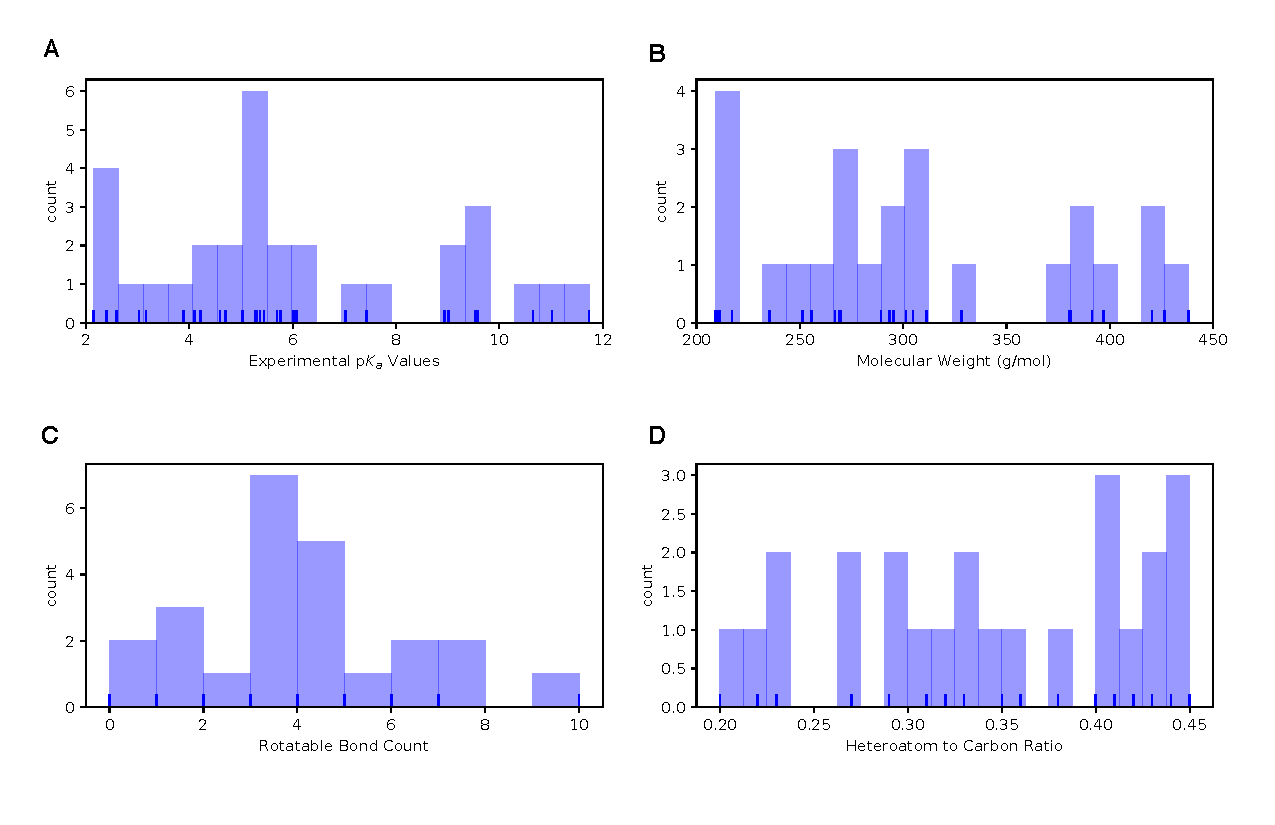
\includegraphics[width=1.0\linewidth]{figures/distribution_of_molecular_properties.pdf}
\caption{{\bf Distribution of molecular properties of 24 compounds in SAMPL6 \pKa{} Challenge.} {\bf A} Histogram of spectrophotometric \pKa{} measurements collected with Sirius T3 ~\cite{Isik:2018:J.Comput.AidedMol.Des.}. Overlayed carpet plot indicates the actual values. Five compounds have multiple measured \pKa{}s in the range of 2-12. {\bf B} Histogram of molecular weights of compounds in SAMPL6 set. Molecular weights were calculated by neglecting counter ions. {\bf C} Histogram of the number of non-terminal rotatable bonds in each molecule. {\bf D} The histogram of the ratio of heteroatom (non-carbon heavy atom) count to the number of carbon atoms.
}
\label{fig:dist_mol_prop}
\end{center}
\end{figure}

The SAMPL6 \pKa{} Challenge was conducted as a blind prediction challenge focus on predicting aqueous \pKa{} value of 24 small molecules that resemble fragments of kinase inhibitors. 
The compound selection process was described in depth in the prior publication reporting SAMPL6 \pKa{} Challenge experimental data collection~\citep{Isik:2018:J.Comput.AidedMol.Des.}.
The distribution of molecular weights, experimental \pKa{} values, number of rotatable bonds, and heteroatom to carbon ratio are depicted in Fig.~\ref{fig:dist_mol_prop}. The challenge molecule set was composed of 17 small molecules with limited flexibility (less than 5 non-terminal rotatable bonds) and 7 molecules with 5-10 non-terminal rotatable bonds. 
The distribution of experimental \pKa{} values ranged between 2-12 and roughly uniform. 
2D representations of all compounds were provided in Fig.~\ref{fig:molecules_with_MAE_of_all_methods}. 
Drug-like molecules are often larger and more complex than the ones used in this study, however, aimed for the

The dataset composition and details of the \pKa{} measurement technique, except the identity of the small molecules, were announced about a month before the challenge start time. 
Experimental macroscopic \pKa{} measurements were collected with spectrophotometric method of Sirius T3, at room temperature in ionic strength-adjusted water with 0.15 M KCl~\citep{Isik:2018:J.Comput.AidedMol.Des.}. 
The instructions for participation and the identity of the challenge molecules were released at the challenge start date (October 25, 2017). 
A table of molecule IDs (in the form of SM\#\#) and	their canonical isomeric SMILES was provided as input.
Blind prediction submissions were accepted until January 22, 2018. 

Following the conclusion of the blind challenge, the experimental data was made public on January 23, 2018. The SAMPL organizers and participants gathered at the Second Joint D3R/SAMPL Workshop, at UC San Diego, La Jolla, CA on February 22-23, 2018 to share results.
The workshop aimed to create an opportunity for participants to have discussions, evaluate the results and lessons of the challenge together. 
The participants reported their results and their own evaluations in the special issue of the Journal of Computer-Aided Molecular Design~\citep{JCAMD_special_issue_pKa}. 

In this first iteration of \pKa{} prediction challenge we were not sure what was the best way to capture all necessary information related to \pKa{} predictions. Our aim was to directly evaluate macroscopic \pKa{} predictions comparing them to experimental macroscopic \pKa{} values and to use collected microscopic \pKa{} prediction data for more in-depth diagnostics of method performance.
Therefore, we asked participants to submit their predictions in three different submission types: 
\begin{itemize}
\item {\bf Type I:} microscopic \pKa{} values and related microstate pairs
\item {\bf Type II:} fractional microstate populations as a function of pH in 0.1 pH increments
\item {\bf Type III:} macroscopic \pKa{} values
\end{itemize}

For each submission type, a machine-readable submission file template was specified. 
For type I submissions, participants were asked to report microstate ID of protonated state, microstate ID of deprotonated state, microscopic \pKa{}, microscopic \pKa{} SEM.  The reason and method of microstate enumeration is discussed further in Section~\ref{section-enumeration-of-microstates} "Enumeration of Microstates".
The SEM captures the statistical uncertainty of the predicted method. 
Microstate IDs were preassigned identifiers for each microstates in the form of SM\#\#\_micro\#\#\#. 
For type II submission, submission format included a table that started with microstate ID and consecutive columns reporting natural logarithm of fractional microstate population values of each predicted microstate for 0.1 pH increments between pH 2 and 12.
For type III submissions participants were asked to report molecule ID, macroscopic \pKa{}, macroscopic \pKa{} SEM.  
It was mandatory to submit predictions for all fields for each prediction, but it was not mandatory to submit predictions for all the molecules or all the submission types. 
Although we have accepted submissions with partial sets of molecules, it would have been a better choice to require predictions for all the  molecules for better comparison of method performance. 
The submission files also included fields for naming the method, listing the software utilized, and a free text method section for the detailed documentation of each method. 

Participants were allowed to submit predictions with multiple methods as long as they create separate submissions files. Anonymous participation to the challenge was allowed, however all participant opted to make their submissions public.
All blind submissions were assigned a unique 5-digit alphanumeric submission ID, which will be used throughout this paper. Unique IDs were also assigned when multiple submissions exists for different submission types of the same method such as microscopic \pKa{}(type I) and macroscopic \pKa{} (type III). 
These submission IDs were also reported in the evaluation papers of participants and allow cross-referencing. Submission IDs, participant provided method names, and method categories are presented in Table~\ref{submission-ID-table}. 
There were many instances that multiple types of submissions of the same method were provided by participants as challenge instructions requested. 
Although each prediction set was assigned a separate submission ID we have matched the submissions that originated from the same method according to the reports of the participant.
Submission ID for both macroscopic (type III) and microscopic (type I) \pKa{} predictions of each method (when exists) are shown in Table~\ref{submission-ID-table}. 





%%%
\subsection{Enumeration of microstates} \label{section-enumeration-of-microstates}

To capture both the \pKa{} value and titration position of microscopic \pKa{} predictions, we needed microscopic \pKa{} predictions to be reported together with the pair of deprotonated and protonated microstates that describes the transition. 
String representations of molecules such as canonical SMILES with explicit hydrogens can be written, however, there can be inconsistencies between the interpretation of canonical SMILES written by different softwares and algorithms.
In order to avoid complications while reading microstate structure files from different sources, we have decided that the safest route was pre-enumerating all possible microstates of challenge compounds, assigning the microstates IDs to each in the form of SM\#\#\_micro\#\#\#, and require participants to report microstate pairs using the provided microstates IDs.   

We enumerated an initial list of microstates with Epik and OpenEye QUACPAC and took the union of results. 
Microstates with Epik were generated using Schrodinger Suite v2016-4, and running Epik to enumerate all tautomers within 20 \pKa{} units of pH 7.
For enumerating microstates with OpenEye QUACPAC, we had to first enumerate formal charges and for each charge enumerate all possible tautomers using the settings of maximum tautomer count 200, level 5, and carbonyl hybridizization False.
Then we created an union of all enumerated states written as canonical isomeric SMILES.
Even though resonance structures correspond to different canonical isomeric SMILES they are not different microstates, therefore it was necessary to remove resonance structures that were replicates of the same tautomer. To detect resonance structures we converted canonical isomeric SMILES to InChI hashes with explicit and fixed hydrogen layer. Structures that describe the same tautomer but different resonance states lead to explicit hydrogen InChI hashes that are identical allowing replicates to be removed. The Jupyter Notebook used for the enumeration of microstates is provided in supplementary documents. Because resonance and geometric isomerism should be ignored when matching predicted structures microstate IDs (except SM20 which should be modelled as E-isomer), we provided microstate ID tables with canonical SMILES and 2D-depictions. 

Despite pooling together enumerated charge states and tautomers with Epik and OpenEye QUACPAC to our surprise the microstate lists were still incomplete.
A better algorithm that can enumerate all possible microstates would be very beneficial. 
In SAMPL6 Challenge participants came up with new microstates that were not present in the initial list that we provided. 
Based on participant requests we iteratively had to update the list of microstates and assign new microstate IDs.
Every time we received a request, we shared the updated microstate ID lists with all the challenge participants.

A working \pKa{} microstate definition for this challenge was provided in challenge instructions for clarity. 
Physically meaningful microscopic \pKa{}s are defined between microstate pairs that can interconvert by single protonation/deprotonation event of only one titrable group. 
So, microstate pairs should have total charge difference of |1| and only one heavy atom that differs in the number of bound hydrogens, regardless of resonance state or geometric isomerism. 
All geometric isomer and resonance structure pairs that have the same number of hydrogens bound to equivalent heavy atoms are related to the same microstate. 
Pairs of resonance structures and geometric isomers (cis/trans, stereo) won't be considered as different microstates, as long as there is no change in the number of hydrogens bound to each heavy atom in these structures.
Since we wanted to participants to report only microscopic \pKa{}s that are describe single deprotonation events (in contrast to transitions between microstates that are different in terms of two or more titratable protons), we have also provided a pre-enumerated list of allowed microstate pairs.

Provided microstate ID and microstate pair lists were intended to be used for reporting microstate IDs and to aid parsing of submissions. 
The enumerated lists of microstates were not created with the intent to guide computational predictions. 
This was clearly stated in the challenge instructions. 
However, we noticed that some participants still used the microstate lists as an input for their \pKa{} predictions as we received complaints from participants that due to our updates to microstate lists they needed to repeat their calculations. 
This would not have been an issue, if participants used \pKa{} prediction protocols that did not rely on an external pre-enumerated list of microstates as an input.
None of the participants have reported this dependency in their method descriptions explicitly, therefore we can not identify which submissions have used the enumerated microstate lists as input and which ones has followed the instructions.




%%%
\subsection{Evaluation approaches}

Since the experimental data for the challenge was mainly composed of macroscopic \pKa{} values of both monoprotic and multiprotic compounds, evaluation of macroscopic and microscopic \pKa{} predictions was not straightforward. For only a subset of 8 molecules, dominant microstate sequence could be inferred from NMR. For the rest of the molecules the only experimental information available was the macroscopic \pKa{} value, while experimental data did not provide any information on which group(s) are being titrated, microcopic \pKa{} values, identity of associated macrostates (which charge) or  microstates (which tautomers). In this comparative performance evaluation of we let the experimental data lead the challenge analysis towards various evaluation routes. To compare macroscopic \pKa{} predictions to experimental values we had to utilize numerical matching algorithms before we could calculate performance statistics. For the subset of molecules with experimental data about microstates, we used microstate  based matching. These matching methods were described further in the next section.

Three types of submissions were collected during the SAMPL6 \pKa{} Challenge. We have only utilized type I (microscopic \pKa{} value and microstate IDs) and type III (macroscopic \pKa{} value) predictions in this article. Type I submissions contained the same prediction information as the the type II submissions which reported fractional population of microstates with respect to pH.


\subsubsection{Matching algorithms for pairing predicted and experimental \pKa{}s}

Macroscopic \pKa{} predictions can be calculated from microscopic \pKa{}s for direct comparison to experimental macroscopic \pKa{} values, although there is still a remaining issue. 
How to match predicted macroscopic \pKa{}s to experimental macroscopic \pKa{}s when there could multiple numbers of each reported for each molecule? 
Experimental data in this case did not provide any information that would indicate the titration site, the overall charge or the tautomer composition of macrostate pairs that are associated with each measured macroscopic \pKa{} that can guide the matching.

For evaluating predictions taking the experimental data as reference Fraczkiewicz et al. deliniated recommendations for fair comparative analysis of computational \pKa{} predictions~\citep{Fraczkiewicz:2013:ReferenceModuleinChemistryMolecularSciencesandChemicalEngineering}. 
In the absence any experimental information that would aid the match, experimental and computational \pKa{}s should be matched preserving the order of \pKa{} values and minimizing sum of absolute errors.

We picked Hungarian matching algorithm~\citep{Kuhn:1955:Nav.Res.Logist.Q., Munkres:1957:JSIAM} to assign experimental and predicted macroscopic \pKa{}s with squared error cost function  as suggested by Kiril Lanevskij. The algorithm is available in SciPy package (\textit{scipy.optimize.linear\_sum\_assignment})~\citep{SciPy-linear-sum-assignment}.
This matching algorithm provides optimum global assignment that minimizes linear sum of squared errors of all pairwise matches.
The reason to select squared error cost function instead of absolute error cost function is to avoid misordered matches,
For instance, for a molecule with experimental \pKa{} values of 4 and 6, and predicted \pKa{}s of 7 and 8, Hungarian matching with absolute error cost function would match 6 to 7 and 4 to 9.
Hungarian matching with squared error cost would match 4 to 7 and 6 to 9, preserving the increasing \pKa{} value order between experimental and predicted values.
A weakness of this approach would be failing to match experimental value of 6 to predicted value of 7, if that was the correct match based on underlying macrostates. But underlying pair of states were unknown to us both because experimental data of the challenge did not contain information about what charge states the transitions were happening between and also because we have not collected the pair of macrostates associated with each \pKa{} predictions in submissions. 
There is no perfect solution to numerical \pKa{} assignment problem, but we tried to determine the most fair way to penalize predictions based on their numerical deviation from the experimental values.

For the analysis of microscopic \pKa{} predictions we adopted a different matching approach. 
Only for the 8 molecules, we utilized the dominant microstate sequence infered from NMR experiments to match computational predictions and experimental \pKa{}s. 
We will refer to this assignment method as microstate matching, where experimental \pKa{} value is matched to the computational microscopic \pKa{} value which was reported for the dominant microstate pair observed for each transition. 
We have compared the results of Hungarian matching and microstate matching. 

Inevitably the choice of matching algorithms to assign experimental and predicted values has an impact on the calculation of performance statistics. We believe the Hungarian algorithm for numerical matching and microstate-based were the best choices, providing the most unbiased matching without introducing assumptions outside of the experimental data.

\subsubsection{Statistical metrics for submission performance}

A variety of accuracy and correlation statistics were considered for analyzing and comparing performance of predictions methods submitted to the SAMPL6 \pKa{} Challenge. 
Calculated performance statistics of predictions were provided to participants before the workshop. 
Details of the analysis and scripts are maintained on the SAMPL6 Github Repository (described in Section \ref{Code-and-Data-Availability}).

There are six error metrics reported for the numerical error of the \pKa{} values: the root-mean-squared error (RMSE), mean absolute error (MAE), mean error (ME), coefficient of determination (R\textsuperscript{2}), linear regression slope (m), and Kendall’s Rank Correlation Coefficient ($\tau$).
Uncertainty in each performance statistic was calculated as 95\% confidence intervals estimated by bootstrapping over predictions with 10000 bootstrap samples. 
Calculated errors statistics of all methods can be found in Table~\ref{SI_statistics_table_macro_pKa} for macroscopic \pKa{} predictions and Tables~\ref{SI-statistics-table-micro-pKa-8mol-microstate} and \ref{SI-statistics-table-micro-pKa-8mol-microstate} for microscopic \pKa{} predictions. 

In addition to the numerical error aspect of the \pKa{} values, we have also evaluated predictions in terms of their ability to capture the correct macrostates (ionization states) and microstates (tautomers of each ionization state) to the extend possible from the available experimental data. 
For macroscopic \pKa{}s experiments did not provide any evidence of the identity of the ionization states. 
However, the number of ionization states indicates the number of macroscopic \pKa{}s that exists between experimental range of 2.0-12.0. 
For instance, SM14 has two experimental \pKa{}s and therefore 3 different charge states were observed between the pH range of 2.0-12.0. 
If a prediction reported 4 macroscopic \pKa{}s, it is clear that this method predicted an extra ionization state. 
With this perspective we reported the number of unmatched experimental \pKa{}s (the number of missing \pKa{} predictions, i.e. missing ionization states) and the number of unmatched predicted \pKa{}s (the number of extra \pKa{} predictions, i.e. extra ionization states) after Hungarian matching. 
The later count was restricted to only predictions with \pKa{} values between 2 and 12, because that was the range of the experimental method. 
Errors in extra or missing \pKa{} prediction errors highlight failure to predict the correct number of ionization states within a pH range.

For the evaluation of microscopic \pKa{} predictions, taking advantage of the available dominant microstate sequence data for a subset of 8 compounds, we calculated the dominant microstate prediction accuracy. Dominant microstate prediction accuracy is the ratio of correct dominant tautomer predictions for each charge state divided by, calculated over all ionization states of each molecule. 
In order to extract the sequence of dominant microstates from the microscopic \pKa{} predictions sets, we calculated the relative free energy of microstates selecting a neutral tautomer and pH 0 as reference following the Equation~\ref{eq:microstate_relative_free_energy}. Calculation of relative free energy of microstates was explained in more detail in a previous publication~\citep{Gunner:2020:J.Comput.AidedMol.Des.}. 

Relative free energy of state with respect to reference state B at pH 0.0 (arbitrary pH value selected as reference) can be calculated as follows: 

\begin{equation}
\Delta G_{AB} = \Delta m_{AB} \:RT\ln{10}\:(pH - pK_{a})
\label{eq:microstate_relative_free_energy}
\end{equation}

$\Delta m_{AB}$ is equal to the number protons in stae A minus state B. R and T indicate molar gas constant and temperature, respectively. 
By calculating relative free energies of all predicted microstates with respect to the same reference state and pH, we were able to determine the sequence of predicted dominant microstates. 
The dominant tautomer of each charge state was determined as the the microstate with the lowest free energy in the subset of predicted microstates of each ionization state. 
This approach is feasible because the relative free energy of tautomers of the same ionization state is independent of pH and therefore the choice of reference pH is arbitrary.

We created a shortlist of top-performing methods for macroscopic and microscopic \pKa{} predictions. Top macroscopic \pKa{} predictions were selected based on the following criteria of consistance performance among different metrics: ranking in the top 10 consistently according to two error (RMSE, MAE) and two correlation metrics (R-Squared, and Kendall’s Tau), and also havin a combined count of less than 8 missing or extra macroscopic \pKa{}s for the entire molecule set (a third of the number of compounds). 
These methods are presented in Table~\ref{typeIII-well-performing-methods-table}. A separate list of top performing methods were selected for microscopic \pKa{} with the following criteria: ranking in the top 10 methods when ranked by accuracy statistics (RMSE and MAE) and perfect dominant microstate prediction accuracy. These methods are presented in Table~\ref{typeI-well-performing-methods-table}.

In addition to comparing the performance comparison of methods, we also wanted to compare \pKa{} prediction performance on the level of molecules to determine \pKa{}s of which molecules in the challenge set were harder to predict considering all the methods in the challenge. 
For this purpose, we plotted prediction error distributions of each molecule considering all prediction methods. 
We also calculated MAE for each molecule’s over all predictions as well as for predictions from each method category. 


%%%
\subsection{Reference calculations}

Including null model as helpful in comparative performance analysis of predictive methods to establish what the performance statistics look like for a baseline method for the specific dataset. 
Null models or null predictions employ a simple prediction model which is not expected to be particularly successful, but it is useful for providing a simple point of comparison for more sophisticated methods. The expectation is for more sophisticated or costly prediction methods to outperform the predictions from a null model, otherwise the simpler null model would be preferable. In SAMPL6 \pKa{} Challenge there were two blind submissions that database lookup methods that were suitable to be considered as null predictions. These methods, with submission IDs \textit{5nm4j} and \textit{5nm4j} both used OpenEye pKa-Porspector database to find the most similar molecule to query molecule and report its \pKa{} as predicted value. 
We acknowledge that database lookup methods with a rich experimental database presents a challenging null model to beat, however, due to the accuracy level needed from \pKa{} predictions for computer-aided drug design we believe it is an appropriate performance baseline that physical and empirical \pKa{} prediction methods should strive to perform better than.

We have also included additional reference calculations in the comparative analysis to provide more perspective. 
The methods we chose to include as reference calculations were missing from the blind predictions sets although they are widely used methods by academia and industry.
representing different methodological approaches: Schrodinger/Epik (\textit{nb007, nb008, nb010}), Schrodinger/Jaguar (\textit{nb011, nb013}), Chemaxon/Chemicalize (\textit{nb015}), and Molecular Discovery/MoKa (\textit{nb016, nb017}). Epik and Jaguar \pKa{} predictions were collected by Bas Rustenburg, Chemicalize predictions by Mehtap Isik, and MoKa predictions by Thomas Fox, after the challenge deadline avoiding any alterations to the respective standard procedures of the methods and guidance of the experimental date. 
Reference calculations were not formally blind, as experimental data of the challenge has been made publically available before their collection. 

All figures and statistics tables in this manuscript include reference calculations. 
As the reference calculations were not formal submissions, these were omitted from formal ranking in the challenge, but we present plots in this article which show them for easy comparison. These are labeled with submission IDs of the form \textit{nb\#\#\#} to allow easy recognition of non-blind reference calculations.

%%%%%%%%%%%%%%%%%%%%%%%%%%%%%%%%%%%%%%%%%%%%%%%%%%%%%%%%%%%%
% Results and Discussion
%%%%%%%%%%%%%%%%%%%%%%%%%%%%%%%%%%%%%%%%%%%%%%%%%%%%%%%%%%%%
\section{Results and Discussion}


Participation to SAMPL6 \pKa{} Challenge was high with 11 research groups contributing \pKa{} prediction sets of 37 methods.  
A large variety of \pKa{} prediction methods were represented in SAMPL6 Challenge. 
We categorized these submissions into four method categories: database lookup (DL), linear free energy relationship (LFER), quantitative structure property relationship or machine learning (QSPR/ML), and quantum mechanics (QM). 
Quantum mechanics models were subcategorized into QM methods with and without linear empirical correction (LEC), and combined quantum mechanics and molecular mechanics (QM + MM). 
Table~\ref{submission-ID-table} presents, method names, submission IDs, method categories, and also references of each approach. 
Integral equation-based approaches (e.g.EC-RISM) were also evaluated under the Physical (QM) category. There were 2 DL, 4 LFER, and 5 QSPR/ML methods represented in the challenge, including the reference calculations. 
Majority of QM calculations include linear empricial corrections (22 methods in QM + LEC category), and only 5 QM methods were submitted without any empirical corrections. 
There were 4 methods that used a mixed physical modeling approach of QM + MM. 

The following sections present detailed performance evaluation of blind submissions and reference prediction methods for macroscopic and microscopic \pKa{} predictions. Performance statistics of all the methods can be found in Tables \ref{SI_statistics_table_macro_pKa} and \ref{SI-statistics-table-micro-pKa-8mol-microstate}. Methods are referred to by their submission ID's which are provided in Table \ref{submission-ID-table}.


\begin{table}%[H]%[tb!]
\begin{center}
\begin{threeparttable}
\centering\scriptsize
\caption{{\bf Submission IDs, names, category, and type for all the \pKa{} prediction sets.} 
Reference calculations are labeled as \textit{nb\#\#\#}. The method name column lists the names provided by each participant in the submission file. The ``type'' column indicates if submission was or a post-deadline reference calculation, denoted by ``Blind'' or ``Reference'' respectively. The methods in the table are grouped by method category and not ordered by performance.  
} 
\label{submission-ID-table}
\begin{tabular}{llllll}
\hline
\textbf{\begin{tabular}[c]{@{}l@{}}Method \\ Category\end{tabular}} & \textbf{Method} & \textbf{\begin{tabular}[c]{@{}l@{}}Microscopic \pKa{} \\ (Type I) \\ Submission ID\end{tabular}} & \textbf{\begin{tabular}[c]{@{}l@{}}Macroscopic \pKa{} \\ (Type III) \\ Submission ID\end{tabular}} & \textbf{\begin{tabular}[c]{@{}l@{}}Submission \\ Type\end{tabular}} & \textbf{Ref.} \\ \hline
\rowcolor[HTML]{EFEFEF} 
DL & Substructure matches to experimental data in pKa OpenEye pKa Prospector Database v1.0 & \textit{} & \textit{5nm4j} & Null & \cite{pKa-prospector-ref} \\
DL & OpenEye pKa-Prospector 1.0.0.3 with Analog Search ion identification algorithm & \textit{} & \textit{pwn3m} & Null & \cite{pKa-prospector-ref} \\
\rowcolor[HTML]{EFEFEF} 
LFER & ACD/pKa GALAS (ACD/Percepta Kernel v1.6) & \textit{v8qph} & \textit{37xm8} & Blind & \cite{ACD-pKa-galas} \\
LFER & ACD/pKa Classic (ACD/Percepta Kernel, v1.6) & \textit{} & \textit{xmyhm} & Blind & \cite{ACD-pKa-classic} \\
\rowcolor[HTML]{EFEFEF} 
LFER & Epik Scan (Schrodinger v2017-4) & \textit{} & \textit{nb007} & Reference & \cite{Shelley:2007:J.Comput.AidedMol.Des.} \\
LFER & Epik Microscopic (Schrodinger v2017-4) & \textit{nb008} & \textit{nb010} & Reference & \cite{Shelley:2007:J.Comput.AidedMol.Des.} \\
\rowcolor[HTML]{EFEFEF} 
QSPR/ML & OpenEye Gaussian Process & \textit{6tvf8} & \textit{hytjn} & Blind & \cite{Bannan:2018:J.Comput.AidedMol.Des.} \\
QSPR/ML & OpenEye Gaussian Process Resampled & \textit{} & \textit{q3pfp} & Blind & \cite{Bannan:2018:J.Comput.AidedMol.Des.} \\
\rowcolor[HTML]{EFEFEF} 
QSPR/ML & S+pKa (ADMET Predictor v8.5, Simulations Plus) & \textit{hdiyq} & \textit{gyuhx} & Blind & \cite{simulation-plus-pKa} \\
QSPR/ML & Chemicalize v18.23 (ChemAxon MarvinSketch v18.23) & \textit{} & \textit{nb015} & Reference & \cite{chemicalize-pKa} \\
\rowcolor[HTML]{EFEFEF} 
QSPR/ML & MoKa v3.1.3 & \textit{nb016} & \textit{nb017} & Reference & \cite{Milletti:2007:J.Chem.Inf.Model., moka-pKa} \\
\rowcolor[HTML]{EFEFEF} 
QM & \begin{tabular}[c]{@{}l@{}}Adiabatic scheme with single point correction:  SMD/M06-2X//6-311++G(d,p)//M06-2X/6-31+G(d) \\ for bases and SMD/M06-2X//6-311++G(d,p)//M06-2X/6-31G(d) for acids  + thermal corrections\end{tabular} & \textit{ko8yx} & \textit{ryzue} & Blind & \cite{Zeng:2018:J.Comput.AidedMol.Des.} \\
QM & \begin{tabular}[c]{@{}l@{}}Direct scheme with single point correction: SMD/M06-2X//6-311++G(d,p)//M06-2X/6-31+G(d) for \\ bases and SMD/M06-2X//6-311++G(d,p)//M06-2X/6-31G(d) for acids  + thermal corrections\end{tabular} & \textit{w4z0e} & \textit{xikp8} & Blind & \cite{Zeng:2018:J.Comput.AidedMol.Des.} \\
\rowcolor[HTML]{EFEFEF} 
QM & \begin{tabular}[c]{@{}l@{}}Adiabatic scheme: thermodynamic cycle that uses gas phase optimized structures for gas phase free \\ energy and solution phase geometries for solvent phase free energy. SMD/M06-2X/6-31+G(d) for \\ bases and SMD/M06-2X/6-31G(d) for acids + thermal corrections\end{tabular} & \textit{wcvnu} & \textit{5byn6} & Blind & \cite{Zeng:2018:J.Comput.AidedMol.Des.} \\
QM & \begin{tabular}[c]{@{}l@{}}Vertical scheme:  thermodynamic cycle that uses only gas phase optimized structures to compute gas \\ hase and solvation free energy. SMD/M06-2X/6-31+G(d) for bases and SMD/M06-2X/6-31G(d) for \\ acids + Thermal corrections\end{tabular} & \textit{arcko} & \textit{w4iyd} & Blind & \cite{Zeng:2018:J.Comput.AidedMol.Des.} \\
\rowcolor[HTML]{EFEFEF} 
QM & \begin{tabular}[c]{@{}l@{}}Direct scheme: solution phase free energy is determined by solution phase geometries  without \\ thermodynamic cycle SMD/M06-2X/6-31+G(d) for bases and SMD/M06-2X/6-31G(d) for acids \\ + thermal corrections\end{tabular} & \textit{wexjs} & \textit{y75vj} & Blind & \cite{Zeng:2018:J.Comput.AidedMol.Des.} \\
QM + LEC & Jaguar (Schrodinger v2017-4) & \textit{nb011} & \textit{nb013} & Reference & \cite{Bochevarov:2013:Int.J.QuantumChem.} \\
\rowcolor[HTML]{EFEFEF} 
QM + LEC & CPCM/B3LYP/6–311+G(d,p) and global fitting & \textit{y4wws} & \textit{35bdm} & Blind & \cite{Selwa:2018:J.Comput.AidedMol.Des.} \\
QM + LEC & \begin{tabular}[c]{@{}l@{}}CPCM/B3LYP/6–311+G(d,p) and separate fitting for neutral to negative and for positive to neutral \\ transformations\end{tabular} & \textit{qsicn} & \textit{p0jba} & Blind & \cite{Selwa:2018:J.Comput.AidedMol.Des.} \\
\rowcolor[HTML]{EFEFEF} 
QM + LEC & EC-RISM/MP2/6-311+G(d,p)-P3NI-q-noThiols-2par & \textit{kxztt} & \textit{ds62k} & Blind & \cite{Tielker:2018:J.Comput.AidedMol.Des.} \\
QM + LEC & EC-RISM/MP2/cc-pVTZ-P2-q-noThiols-2par & \textit{ftc8w} & \textit{2ii2g} & Blind & \cite{Tielker:2018:J.Comput.AidedMol.Des.} \\
\rowcolor[HTML]{EFEFEF} 
QM + LEC & EC-RISM/MP2/6-311+G(d,p)-P2-phi-all-2par & \textit{ktpj5} & \textit{nb001} & Blind* & \cite{Tielker:2018:J.Comput.AidedMol.Des.} \\
QM + LEC & EC-RISM/MP2/6-311+G(d,p)-P2-phi-noThiols-2par & \textit{wuuvc} & \textit{nb002} & Blind* & \cite{Tielker:2018:J.Comput.AidedMol.Des.} \\
\rowcolor[HTML]{EFEFEF} 
QM + LEC & EC-RISM/MP2/6-311+G(d,p)-P3NI-phi-all-2par & \textit{2umai} & \textit{nb003} & Blind* & \cite{Tielker:2018:J.Comput.AidedMol.Des.} \\
QM + LEC & EC-RISM/MP2/6-311+G(d,p)-P3NI-phi-noThiols-2par & \textit{cm2yq} & \textit{nb004} & Blind* & \cite{Tielker:2018:J.Comput.AidedMol.Des.} \\
\rowcolor[HTML]{EFEFEF} 
QM + LEC & EC-RISM/MP2/6-311+G(d,p)-P2-phi-all-1par & \textit{z7fhp} & \textit{nb005} & Blind* & \cite{Tielker:2018:J.Comput.AidedMol.Des.} \\
QM + LEC & EC-RISM/MP2/6-311+G(d,p)-P3NI-phi-all-1par & \textit{8toyp} & \textit{nb006} & Blind* & \cite{Tielker:2018:J.Comput.AidedMol.Des.} \\
\rowcolor[HTML]{EFEFEF} 
QM + LEC & EC-RISM/MP2/cc-pVTZ-P2-phi-noThiols-2par & \textit{epvmk} & \textit{ttjd0} & Blind & \cite{Tielker:2018:J.Comput.AidedMol.Des.} \\
QM + LEC & EC-RISM/MP2/cc-pVTZ-P2-phi-all-2par & \textit{xnoe0} & \textit{mkhqa} & Blind & \cite{Tielker:2018:J.Comput.AidedMol.Des.} \\
\rowcolor[HTML]{EFEFEF} 
QM + LEC & EC-RISM/MP2/cc-pVTZ-P3NI-phi-noThiols-2par & \textit{4o0ia} & \textit{mpwiy} & Blind & \cite{Tielker:2018:J.Comput.AidedMol.Des.} \\
QM + LEC & EC-RISM/B3LYP/6-311+G(d,p)-P3NI-q-noThiols-2par & \textit{nxaaw} & \textit{ad5pu} & Blind & \cite{Tielker:2018:J.Comput.AidedMol.Des.} \\
\rowcolor[HTML]{EFEFEF} 
QM + LEC & EC-RISM/B3LYP/6-311+G(d,p)-P3NI-phi-noThiols-2par & \textit{0xi4b} & \textit{f0gew} & Blind & \cite{Tielker:2018:J.Comput.AidedMol.Des.} \\
QM + LEC & EC-RISM/B3LYP/6-311+G(d,p)-P2-phi-noThiols-2par & \textit{cywyk} & \textit{np6b4} & Blind & \cite{Tielker:2018:J.Comput.AidedMol.Des.} \\
\rowcolor[HTML]{EFEFEF} 
QM + LEC & PCM/B3LYP/6-311+G(d,p) & \textit{gdqeg} & \textit{yc70m} & Blind & \cite{Tielker:2018:J.Comput.AidedMol.Des.} \\
QM + LEC & COSMOtherm\_FINE17 (COSMOtherm C30\_1701, BP/TZVPD/FINE//BP/TZVP/COSMO) & \textit{t8ewk} & \textit{0hxtm} & Blind & \cite{Klamt:2003:J.Phys.Chem.Ab, Eckert:2006:J.Comput.Chem.} \\
\rowcolor[HTML]{EFEFEF} 
QM + LEC & \begin{tabular}[c]{@{}l@{}}DSD-BLYP-D3(BJ)/def2-TZVPD//PBEh-3c[DCOSMO-RS] + RRHO(GFN-xTB[GBSA]) \\ + Gsolv(COSMO-RS[TZVPD]) and linear fit\end{tabular} & \textit{} & \textit{xvxzd} & Blind & \cite{Pracht:2018:J.Comput.AidedMol.Des.} \\
QM + LEC & \begin{tabular}[c]{@{}l@{}}ReSCoSS conformations // DSD-BLYP-D3 reranking // COSMOtherm pKa:  DSD-BLYP-D3(BJ)/\\ def2-TZVPD// PBE-D3(BJ)/def2-TZVP/COSMO + RRHO[GFN-xTB + GBSA-water] \\ + Gsolv[COSMO-RS(FINE17/TZVPD)] level and COSMOtherm pKa applied  at the single conformer \\ pair level  (COSMOthermX17.0.5 release and BP-TZVPD-FINE-C30-1701 parameterization)\end{tabular} & \textit{eyetm} & \textit{8xt50} & Blind & \cite{Pracht:2018:J.Comput.AidedMol.Des.} \\
\rowcolor[HTML]{EFEFEF} 
QM + LEC & \begin{tabular}[c]{@{}l@{}}ReSCoSS conformations // COSMOtherm pKa: DSD-BLYP-D3(BJ)/def2-TZVPD// PBE-D3(BJ)/\\ def2-TZVP/COSMO + RRHO[GFN-xTB + GBSA-water] + Gsolv[COSMO-RS(FINE17/TZVPD)] \\ level and COSMOtherm pKa was applied directly on the resulting conformer sets with at least 5\% \\ Boltzmann weights for each microspecies (COSMOthermX17.0.5 release and BP-TZVPD-FINE-\\ C30-1701 parameterization)\end{tabular} & \textit{ccpmw} & \textit{yqkga} & Blind & \cite{Pracht:2018:J.Comput.AidedMol.Des.} \\
QM + MM & \begin{tabular}[c]{@{}l@{}}M06-2X/6-31G*(for bases) or 6-31+G*(for acids) for gas phase, solvation free energy using TI with \\ explicit solvent and GAFF, solvation free energy of proton -265.6 kcal/mol\end{tabular} & \textit{0wfzo} & \textit{} & Blind & \cite{Prasad:2018:J.Comput.AidedMol.Des.} \\
\rowcolor[HTML]{EFEFEF} 
QM + MM & \begin{tabular}[c]{@{}l@{}}M06-2X/6-31G*(for bases) or 6-31+G*(for acids) for gas phase, solvation free energy using TI with \\ explicit solvent and GAFF, solvation free energy of proton -271.88 kcal/mol\end{tabular} & \textit{z3btx} & \textit{} & Blind &  \\
QM + MM & \begin{tabular}[c]{@{}l@{}}M06-2X/6-31G*(for bases) or 6-31+G*(for acids) + thermal state correction for gas phase,  solvation \\ free energy using TI with explicit solvent and GAFF, solvation free energy of proton -265.6 kcal/mol\end{tabular} & \textit{758j8} & \textit{} & Blind &  \\
\rowcolor[HTML]{EFEFEF} 
QM + MM & \begin{tabular}[c]{@{}l@{}}M06-2X/6-31G*(for bases) or 6-31+G*(for acids) + thermal state correction for gas phase, solvation \\ free energy using TI with explicit solvent and GAFF, solvation free energy of proton -271.88 kcal/mol\end{tabular} & \textit{hgn83} & \textit{} & Blind &  \\ \hline
\end{tabular}
\begin{tablenotes}
\item[*] Microscopic \pKa{} submissions were blind, however, participant requested a correction after blind submission deadline for macroscopic \pKa{} submissions. Therefore, these were assigned submission IDs in the form of \textit{nb\#\#\#}.
\end{tablenotes}
\end{threeparttable}
\end{center}
\end{table}



%%%
\subsection{Analysis of macroscopic \pKa{} predictions}

\begin{figure}[h]
\centering
%\makebox[\textwidth][l]{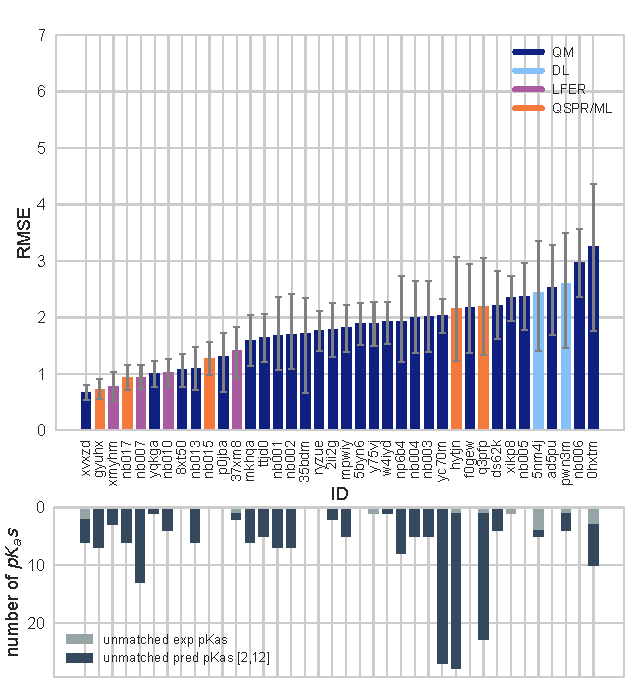
\includegraphics[width=0.5\textwidth]{figures/typeIII-rmse-unmatched-pKa-fig.pdf}}
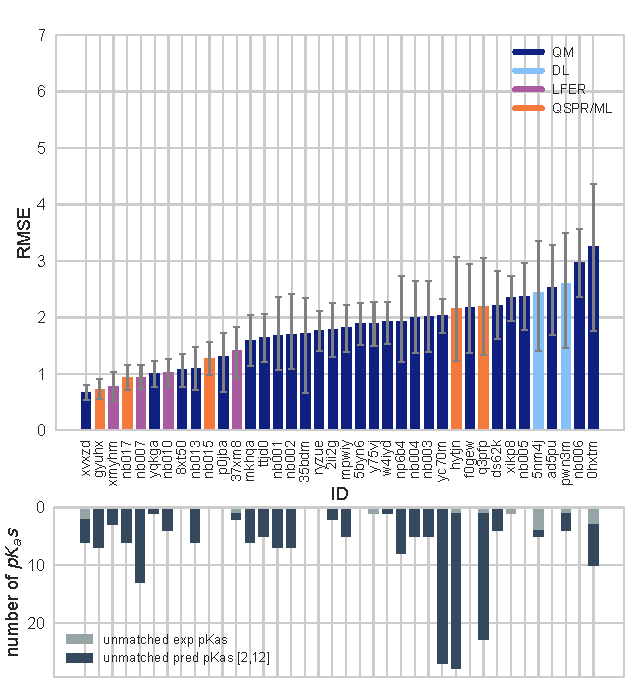
\includegraphics[width=0.5\linewidth]{figures/typeIII-rmse-unmatched-pKa-fig.pdf}
\caption{{\bf RMSE and unmatched \pKa{} counts vs. submission ID plots for macroscopic \pKa{} predictions based on Hungarian matching.} 
Methods are indicated by submission IDs. 
RMSE is shown with error bars denoting 95\% confidence intervals obtained by bootstrapping over challenge molecules. 
Submissions are colored by their method categories. Light blue colored database look up methods are utilized as the null prediction method.
QM methods (navy) includes pure QM, QM+LEC, and QM+MM approaches.
Lower bar plots show the number of unmatched experimental \pKa{}s (light grey, missing predictions) and the number of unmatched \pKa{} predictions (dark grey, extra predictions) for each method between pH 2 and 12. Submission IDs are summarized in Table~\ref{submission-ID-table}. Submission IDs of the form \textit{nb\#\#\#} refer to non-blinded reference methods computed after the blind challenge submission deadline. All others refer to blind, prospective predictions. 
}
\label{fig:typeIII-rmse-plot}
\end{figure}

The performance of macroscopic \pKa{} predictions were analyzed by comparison to experimental \pKa{} values collected by the spectrophotometric method via numerical matching following the Hungarian method.  
Overall \pKa{} prediction performance was lower than we have hoped for. 
Fig.~\ref{fig:typeIII-rmse-plot} shows RMSE calculated for each prediction method represented by their submission IDs. 
Other performance statistics are depicted in Fig.~\ref{fig:typeIII-statistics}.
In both figures method categories were indicated by the color of the error bars.  Statistics depicted in these figures can be found in Table~\ref{SI_statistics_table_macro_pKa}.
Prediction error ranged between 0.7 to 3.2 \pKa{} units in terms of RMSE, while an RMSE between 2-3 log units was observed for the majority of methods (20 out of 38 methods). 
Only five methods achieved RMSE less than 1 \pKa{} unit. One is QM method with COSMO-RS approach for solvation and linear empirical correction (\textit{xvxzd} (DSD-BLYP-D3(BJ)/def2-TZVPD//PBEh-3c[DCOSMO-RS] + RRHO(GFN-xTB[GBSA]) + Gsolv(COSMO-RS[TZVPD]) and linear fit)), and the remaining four are empirical prediction methods of LFER (\textit{xmyhm} (ACD/pKa Classsic), \textit{nb007} (Schrodinger/Epik Scan)) and QSPR/ML categories (\textit{gyuhx} (Simulations Plus), \textit{nb017} (MoKa)). 
These five methods with RMSE less than 1 \pKa{} unit also are the methods that have the lowest MAE.
\textit{xmyhm} and \textit{xvxzd} were the only two methods for which the upper 95\% confidence interval of RMSE was lower than 1 \pKa{} unit. 

In terms of correlation statistics performance of many methods have good performance, although the ranking of methods change R\textsuperscript{2} and Kendall's Tau and many methods are indistinguishable from one another considering uncertainty of the correlation statistics. 
32 out of 38 methods have R\textsuperscript{} higher than and Kendall's Tau higher than 0.7 and 0.6, respectively.
8 methods have R\textsuperscript{2} higher than 0.9 and 6 methods have Kendall's Tau higher than 0.8.
The overlap of these two sets are the following:
\textit{gyuhx} (Simulations Plus), \textit{xvxzd} (DSD-BLYP-D3(BJ)/def2-TZVPD//PBEh-3c[DCOSMO-RS] + RRHO(GFN-xTB[GBSA]) + Gsolv(COSMO-RS[TZVPD]) and linear fit), \textit{xmyhm} (ACD/pKa Classic), \textit{ryzue} (Adiabatic scheme with single point correction: MD/M06-2X//6-311++G(d,p)//M06-2X/6-31+G(d) for bases and SMD/M06-2X//6-311++G(d,p)//M06-2X/6-31G(d) for acids + thermal corrections), and \textit{5byn6} 
(Adiabatic scheme: thermodynamic cycle that uses gas phase optimized structures for gas phase free energy and solution phase geometries for solvent phase free energy. SMD/M06-2X/6-31+G(d) for bases and SMD/M06-2X/6-31G(d) for acids + thermal corrections).
It is worth noting that the \textit{ryzue} and \textit{5byn6} are QM predictions without any empirical correction. Their high correlation and rank correlation coefficient scores signal that with an empirical correction their accuracy based performance could improve. Indeed, the participants have showed that this is the case in their individual challenge analysis paper and achieved RMSE of 0.73 \pKa{} units after the challenge~\citep{Zeng:2018:J.Comput.AidedMol.Des.}. 

Null prediction methods based on database lookup (\textit{5nm4j} and \textit{pwn3m}) had similar performance, roughly RMSE of 2.5 \pKa{} units, MAE of 1.5 \pKa{} units, R\textsuperscript{2} of 0.2 and Kendall's Tau of 0.3.
Many methods were observed to have prediction performance advantage over the Null predictions shown in light blue in Fig.~\ref{fig:typeIII-rmse-plot} and Fig.~\ref{fig:typeIII-statistics} considering all the performance metrics as a whole.
In terms of correlation statistics the null methods are the worst performers, except \textit{0hxtm}.
From the perspective of accuracy-based statistics (RMSE and MAE), only the top 10 methods were observed to have significantly lower errors than the null methods considering the uncertainty of error metrics expressed as 95\% confidence intervals.

Distribution of macroscopic \pKa{} prediction signed errors observed in each submission was plotted in Fig.~\ref{fig:typeIII-error-distribution}A as ridge plots based on Hungarian matching.
\textit{2ii2g, f0gew, np64b, p0jba}, and \textit{yc70m} tend to overestimate and \textit{
5byn6, ryzue}, and \textit{w4iyd} tend to underestimate macroscopic \pKa{} values. 

There were four submissions of QM+LEC category that used COSMO-RS implicit solvation model. 
It was interesting that while three of these achieved the lowest RMSE among QM-based methods (\textit{xvxzd}, \textit{yqkga}, and \textit{8xt50})~\citep{Pracht:2018:J.Comput.AidedMol.Des.} and one of them showed the highest RMSE (\textit{0hxtm} (COSMOtherm\_FINE17)) in SAMPL6 Challenge macroscopic \pKa{} predictions. 
All four methods used COSMO-RS/FINE17 level to compute solvation free energies. The major difference between the three low-RMSE methods and the \textit{0hxtm} seems to be the protocol for determining relevant conformations for each microstate. 
\textit{xvxzd}, \textit{yqkga}, and \textit{8xt50} methods used semi-empirical tight binding (GFN-xTB) method and GBSA continuum solvation model for geometry optimization of conformers and followed up with high level single point energy calculations with solvation free energy (COSMO-RS(FINE17/TZVPD)) and rigid rotor harmonic oscilator (RRHO[GFN-xTB(GBSA]) corrections. 
\textit{yqkga}, and \textit{8xt50} methods selected  conformations for each microstate with Relevant Solution Conformer Sampling and Selection (ReSCoSS) workflow. Conformations were clustered according to shape and lowest energy conformations from each cluster according to BP86/TZVP/COSMO single point energies in any of the 10 different COSMO-RS solvents were considered as relevant conformers. More details of the ReSCoSS workflow was described by Pracht et al~\citep{Pracht:2018:J.Comput.AidedMol.Des.}
\textit{yqkga} method further filtered out conformers that have less than 5\% Boltzmann weights at the DSD-BLYP-D3/def2-TZVPD + RRHO(GFNxTB) + COSMO-RS(fine) level.
\textit{xvxzd} method used MF–MD–GC//GFN-xTB workflow and used energy thresholds of 6 kcal/mol and 10 kcal/mol, for conformer and microstate selection
On the other hand, the comformational ensemble captured for each microstate seems to be much limited for \textit{0hxtm} method, judging by the method description in the submission file. \textit{0hxtm} method reported that relevant conformations were computed with the COSMOconf 4.2 workflow which produced multiple relevant conformers for only the neutral states of SM18 and SM22.  
In contrast to \textit{xvxzd}, \textit{yqkga}, and \textit{8xt50} methods, the \textit{0hxtm} method also did not include a RRHO correction.
Participants of the three low-RMSE methods report that capturing the chemical ensemble for each molecule including conformers and tautomers and high level QM calculations led to more successful macroscopic \pKa{} prediction results and RRHO correction provided a minor improvement~\citep{Pracht:2018:J.Comput.AidedMol.Des.}. Comparing these results to other QM approaches in SAMPL Challenge also points to the advantage of COSMO-RS solvation approach compared to other implicit solvent models.

In addition the statistics related to the value of \pKa{}, we have also analyzed missing or extra \pKa{} predictions. 
Analysis of the \pKa{} values with accuracy- and correlation-based error metrics was only possible after assignment of predicted macroscopic \pKa{}s to experimental \pKa{}s through the Hungarian matching, although, this approach masks \pKa{} prediction issues in the form of extra or missing macroscopic \pKa{} predictions. 
To capture this form of prediction errors we reported the number of unmatched experimental \pKa{}s (missing \pKa{} predictions and the number of unmatched predicted \pKa{}s (extra \pKa{} predictions) after Hungarian matching for each method. 
Both missing and extra \pKa{} prediction counts were only considered for the pH range of 2-12 which was the limits of experimental measurements.
The lower subplot of Fig.~\ref{fig:typeIII-rmse-plot} shows the total count of unmatched experimental or predicted \pKa{}s for all the molecules in each prediction set. The order of submission IDs in the x-axis follows the RMSD based ranking so that the performance of each methods from both \pKa{} value accuracy and the number of \pKa{}s can be viewed together.
Presence of missing or extra macroscopic \pKa{} predictions is a critical error, because inaccuracy in predicting the correct number of macroscopic transitions shows that methods are failing predict the correct set of charge states, i.e. failing to predict the correct number of ionization states that can be observed between the specificied pH range. 

In challenge results, extra macroscopic \pKa{} predictions were found to be more common than missing \pKa{} predictions. 
In \pKa{} prediction evaluations usually accuracy of ionization states predicted within a pH range seen is neglected. 
When predictions are only evaluated for \pKa{} value accuracy with numerical matching algorithms more \pKa{} predictions are likely to lead to lower prediction errors. 
Therefore, it is not surprising that methods are biased to predict extra \pKa{} values. 
The SAMPL6 \pKa{} Challenge experimental data consists of 31 macroscopic \pKa{}s in total, measured for 24 molecules (6 molecules in the set have multiple \pKa{}s).
Within the 10 methods with lowest RMSE only \textit{xvxzd} method has an error of missing predicted \pKa{} (2 unmatched out of 31 experimental \pKa{}s), and all other methods that rank top 10 according to RMSE have extra predicted \pKa{}s ranging from 1 to 13. Two prediction sets without any extra \pKa{} predictions and low RMSE are \textit{8xt50} (ReSCoSS conformations // DSD-BLYP-D3 reranking // COSMOtherm pKa) and \textit{nb015} (ChemAxon/Chemicalize).



\begin{figure}[ht!]
\centering
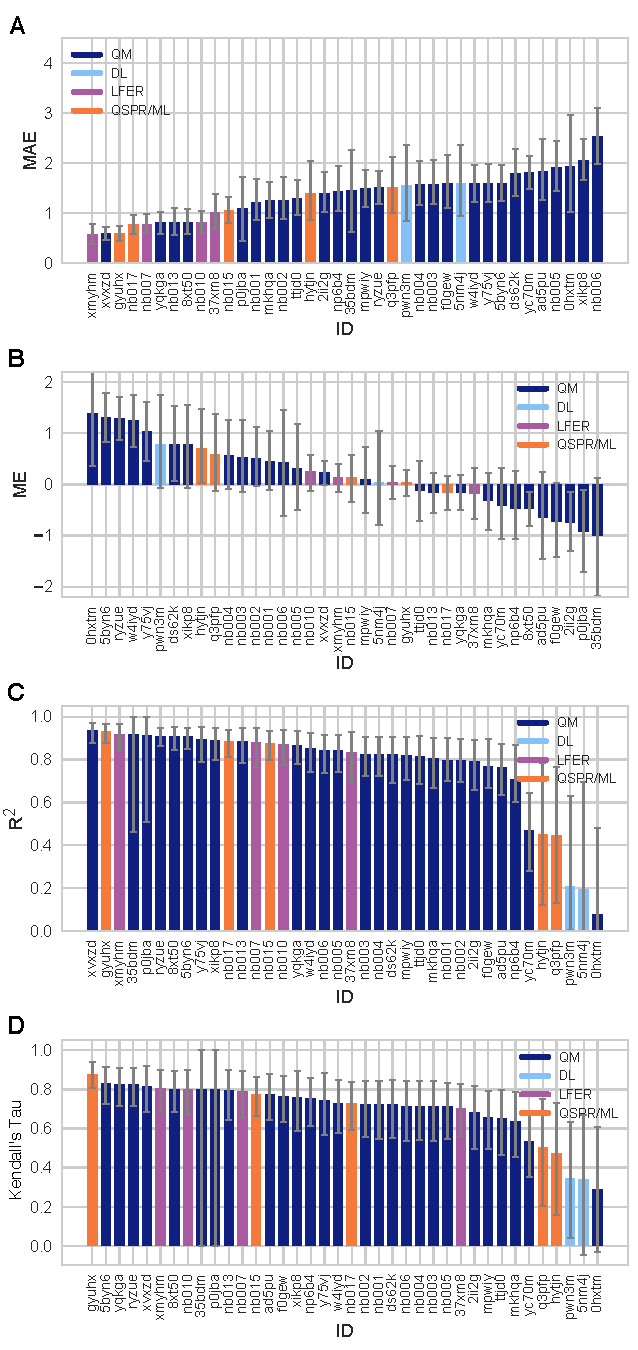
\includegraphics[width=0.5\linewidth]{figures/typeIII_statistics.pdf}
\caption{{\bf Additional performance statistics for macrocopic \pKa{} predictions based on Hungarian matching.} 
Methods are indicated by submission IDs. 
Mean absolute error (MAE), mean error (ME), Pearson’s R\textsuperscript{2}, and Kendall’s Rank Correlation Coefficient Tau ($\tau$) are shown, with error bars denoting 95\% confidence intervals obtained by bootstrapping over challenge molecules. Refer to Table~\ref{submission-ID-table} for submission IDs and method names. Submissions are colored by their method categories. Light blue colored database look up methods are utilized as the null prediction method.
}
\label{fig:typeIII-statistics}
\end{figure}


\subsubsection{Consistently well performing methods for macroscopic \pKa{} prediction}

Methods ranked differently when ordered by different error metrics, although there were a couple of methods that consistently ranked at the top fraction. 
By using a combinatorial criteria that takes all multiple statistical metrics and unmatched \pKa{} counts into account, we identified a short list of consistently well performing methods for macroscopic \pKa{} predictions, shown in Table~\ref{typeIII-well-performing-methods-table}. 
The criteria for selection was ranking in Top 10 according to RMSE, MAE, R\textsuperscript{2}, and Kendall's Tau and also having a combined unmatched \pKa{} (extra and missing \pKa{}s) count less than 8 (a third of the number of compounds).
The resulted in a list of four methods which are consistently well performing across all criteria.

Consistently well performing methods for macroscopic \pKa{} prediction included methods from all categories. Two methods of the QM+LEC category were \textit{xvxzd} (DSD-BLYP-D3(BJ)/def2-TZVPD//PBEh-3c[DCOSMO-RS] + RRHO(GFN-xTB[GBSA]) + Gsolv(COSMO-RS[TZVPD]) and linear fit) and \textit(8xt50) (ReSCoSS conformations // DSD-BLYP-D3 reranking // COSMOtherm pKa) and both used COSMO-RS approach. 
Empirical \pKa{} predictions with top performance were both proprietary softwares. 
From QSPR and LFER categories, \textit{gyuhx} (Simulation Plus) and \textit{xmymhm} (ACD/pKa Classic) were the methods that made it to consistently well performing methods list. Simulation Plus \pKa{} prediction method consisted of 10 artificial neural network ensembles trained on 16,000 compounds for 10 classes of ionizable atoms. Atom type and local molecular environment was how the ionization class of each atom was determined ~\citep{simulation_plus_D3R_presentation}. 
ACD/pKa Classic which was trained on method 17,000 compounds uses Hammet-type equations and tries to capture effects related to tautomeric equilibria, covalent hydration, resonance effects, and  $\alpha, \beta$-unsaturated systems ~\citep{ACD-pKa-classic}.


\begin{table}[h]
\begin{center}
\begin{threeparttable}
\centering\scriptsize
\caption{{\bf Four consistently well-performing prediction methods for macroscopic \pKa{} prediction based on consistent ranking within the Top~10 according to various statistical metrics.} 
Submissions were ranked according to RMSE, MAE, R\textsuperscript{2}, and $\tau$. Consistently well-performing methods were selected as the ones that rank in the Top~10 in each of these statistical metrics. These methods also have less than 2 unmatched experimental \pKa{}s and less than 7 unmatched predicted \pKa{}s according to Hungarian matching. Performance statistics are provided as mean and 95\% confidence intervals.
} 
\label{typeIII-well-performing-methods-table}
\begin{tabular}{@{}llllllll@{}}
\toprule
\textbf{Submission ID} & \textbf{Method Name} & \textbf{RMSE} & \textbf{MAE} & \textbf{R\textsuperscript{2}} & \textbf{\begin{tabular}[c]{@{}l@{}}Kendall's Tau \\ ($\tau$)\end{tabular}} & \textbf{\begin{tabular}[c]{@{}l@{}}Unmatched Exp. \\ \pKa{} Count\end{tabular}} & \textbf{\begin{tabular}[c]{@{}l@{}}Unmatched Pred. \\ \pKa{} Count [2,12]\end{tabular}} \\ \midrule
\rowcolor[HTML]{EFEFEF} 
\textit{xvxzd} & \begin{tabular}[c]{@{}l@{}}Full quantum chemical calculation of \\ free energies and fit to experimental pKa\end{tabular} & 0.68 [0.54, 0.81] & 0.58 [0.45, 0.71] & 0.94 [0.88, 0.97] & 0.82 [0.68, 0.92] & 2 & 4 \\
\textit{gyuhx} & S+pKa & 0.73 [0.55, 0.91] & 0.59 [0.44, 0.74] & 0.93 [0.88, 0.96] & 0.88 [0.8, 0.94] & 0 & 7 \\
\rowcolor[HTML]{EFEFEF} 
\textit{xmyhm} & ACD/pKa Classic & 0.79 [0.52, 1.03] & 0.56 [0.38, 0.77] & 0.92 [0.85, 0.97] & 0.81 [0.68, 0.9] & 0 & 3 \\
\textit{8xt50} & \begin{tabular}[c]{@{}l@{}}ReSCoSS conformations // DSD-BLYP-D3 \\ reranking // COSMOtherm pKa\end{tabular} & 1.07 [0.78, 1.36] & 0.81 [0.58, 1.07] & 0.91 [0.84, 0.95] & 0.80 [0.68, 0.89] & 0 & 0 \\ \bottomrule
\end{tabular}
\end{threeparttable}
\end{center}
\end{table}

In Figure~\ref{fig:typeIII_pred_vs_exp_correlation} prediction vs. experimental data correlation plots of macroscopic \pKa{} predictions with 4 consistently well-performing methods, a representative average method, and the null method(\textit{5nm4j}). The representative method with average performance (\textit{2ii2g} (EC-RISM/MP2/cc-pVTZ-P2-q-noThiols-2par)) was selected as the method with the highest RMSE below the median of all methods.

\begin{figure}[h]
\centering
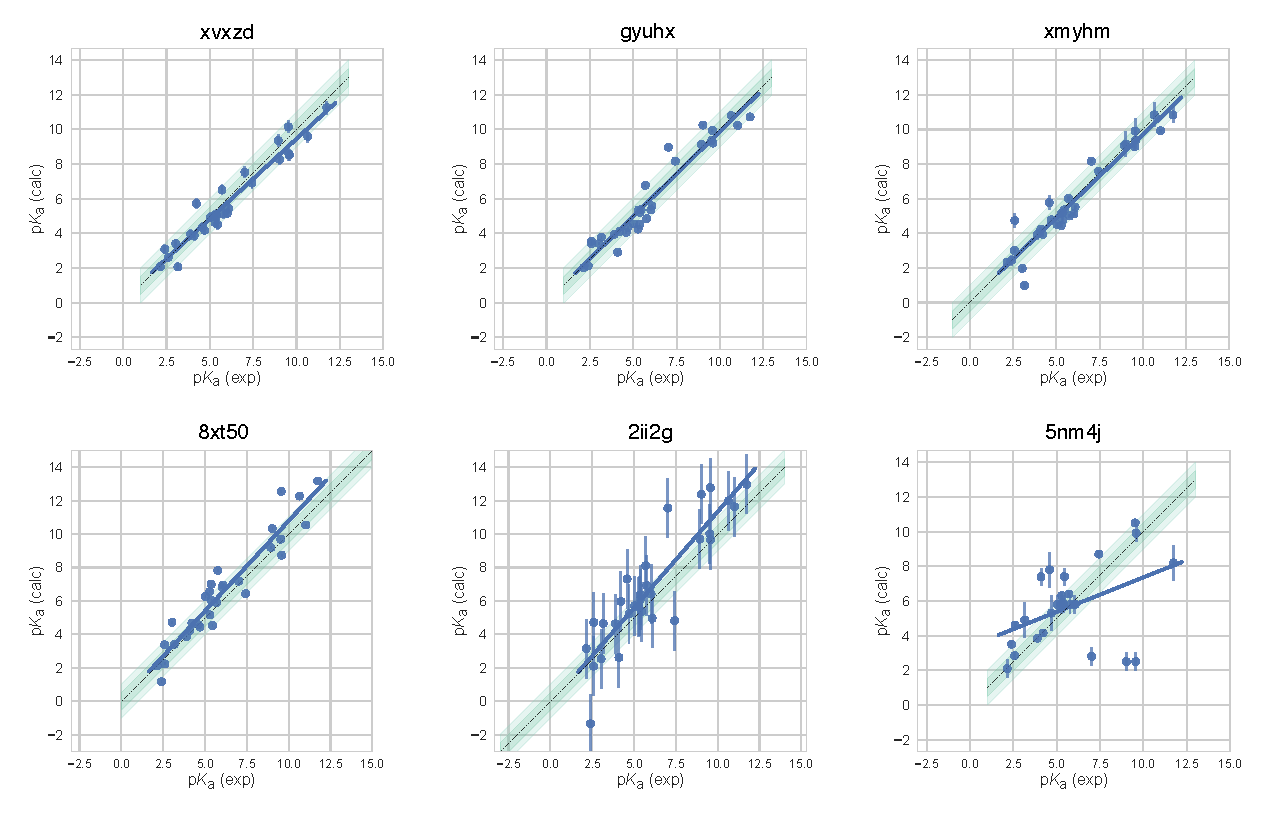
\includegraphics[width=1.0\linewidth]{figures/typeIII-pred-vs-exp-correlation-fig.pdf}
\caption{{\bf Predicted vs. experimental value correlation plots of 4 consistently well-performing methods, a representative method with average performance (\textit{2ii2g}), and the null method (\textit{5nm4j})}. 
Dark and light green shaded areas indicate 0.5 and 1.0 units of error. Error bars indicate standard error of the mean of predicted and experimental values. Experimental \pKa{} SEM values are too small to be seen under the data points. EC-RISM/MP2/cc-pVTZ-P2-q-noThiols-2par method (\textit{2ii2g}) was selected as the representative method with average performance because it is the method with the highest RMSE below the median.
}
\label{fig:typeIII_pred_vs_exp_correlation}
\end{figure}



\subsubsection{Which chemical properties are driving macroscopic \pKa{} prediction failures?}

In addition to comparing the performance of methods that participated in the SAMPL6 Challenge, we also wanted to analyze macroscopic \pKa{} predictions from the perspective of challenge molecules and determine whether particular compounds suffer from larger inaccuracy in \pKa{} predictions. 
The goal of this analysis is to provide guidance on which molecular properties or moieties might be causing larger \pKa{} prediction error.
In Fig.~\ref{fig:molecules_with_MAE_of_all_methods} 2D depictions of challenge molecules are presented with MAE calculated for their macroscopic \pKa{} predictions over all methods, based on Hungarian match. For multiprotic molecules MAE was averaged over all the \pKa{}s. For the analysis of \pKa{} predictiona accuracy observed for each molecule, MAE is a more appropriate statistical value than RMSE for following global trends. This is because MAE value less sensitive to outliers than is RMSE.


A comparison of prediction performance of individual molecules is shown in Fig.~\ref{fig:typeIII_molecular_MAE}. In Fig.~\ref{fig:typeIII_molecular_MAE}A MAE each molecule is shown  considering all blind predictions and reference calculations. A cluster of molecules marked orange and red have higher than average MAE. 
Molecules marked red (SM06, SM21, and SM22) are the only compounds in SAMPL6 dataset with bromo or iodo groups and they suffered a macroscopic \pKa{} prediction error in the range of 1.7-2.0 \pKa{} units in terms of MAE.
Molecules marked orange (SM03, SM10, SM18, SM19, and SM20) all have sulfur-containing heterocycles, and all molecules except SM18 of this group have MAE larger than 1.6 \pKa{} unit.
SM18 despite containing thiazole group has a low MAE. SM18 is the only compound with three experimental \pKa{}s and we suspect presence of multiple experimental \pKa{}s could have a masking affect on the errors captured by MAE with Hungarian matching due to more pairing choices.

We analyzing MAE of each molecule for empirical(LFER and QSPR/ML) and QM-based physical methods (QM, QM+LEC, and QM+MM) separetely for more insight. 
Fig.~\ref{fig:typeIII_molecular_MAE}B shows that the difficulty of predicting \pKa{}s of the same subset of molecules was a trend conserved in the performance of physical methods. For QM-based methods too sulfur containing heterocycles, amide next to aromatic heterocycles, compounds with iodo and bromo domains have lower \pKa{} prediction accuracy.

SAMPL6 \pKa{} set consists of only 24 small molecules which limits our ability to do statistically confirm the determination of which chemical substructures cause greater errors in \pKa{} predictions. Still the trends seen in this challenge distinguish molecules with iodo, bromo, and sulfur-containing heterocycles with larger prediction errors of macroscopic \pKa{} value. We hope that reporting this observation will lead to improvement of methods for similar compounds with such moieties. 


\begin{figure}
\begin{center}
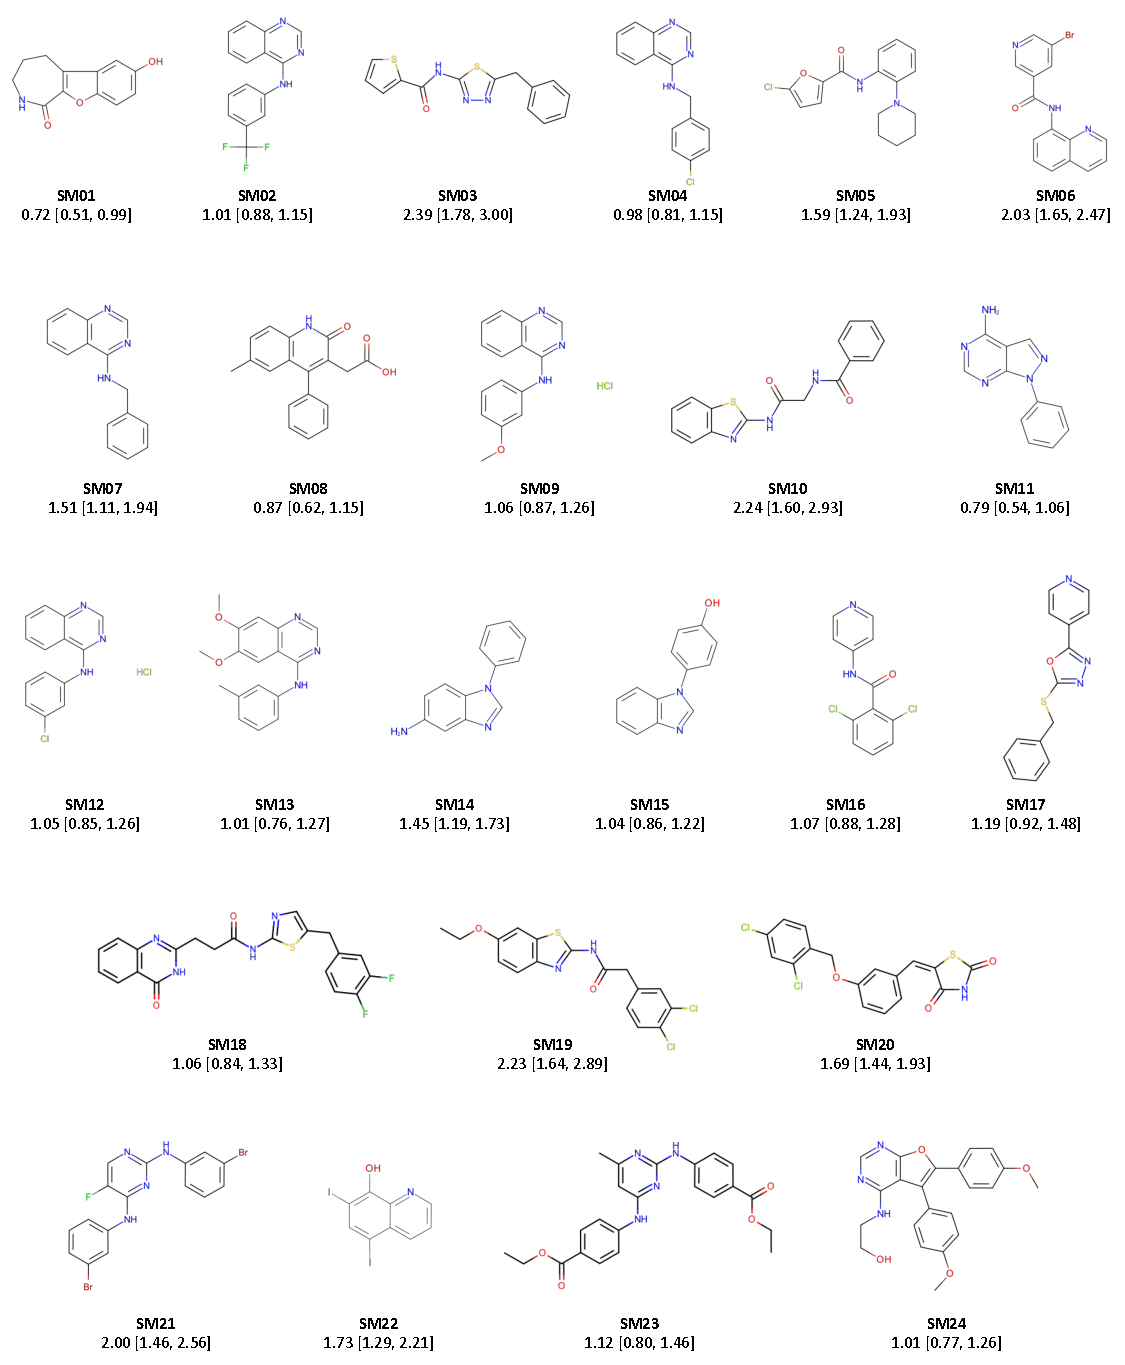
\includegraphics[width=0.95\linewidth]{figures/molecules_with_MAE_of_all_methods.pdf}
\caption{{\bf Molecules of SAMPL6 Challenge with MAE calculated for all macroscopic \pKa{} predictions.} MAE calculated considering all prediction methods indicate which molecules had the lowest prediction accuracy in SAMPL6 Challenge. MAE values calculated for each molecule include all the matched \pKa{} values, which could be more than one per method for multiprotic molecules (SM06, SM14, SM15, SM16, SM18, SM22). Hungarian matching algorithm was employed for pairing experimental and predicted \pKa{} values. MAE values are reported with 95\% confidence intervals.
}
\label{fig:molecules_with_MAE_of_all_methods}
\end{center}
\end{figure}


\begin{figure}
\centering
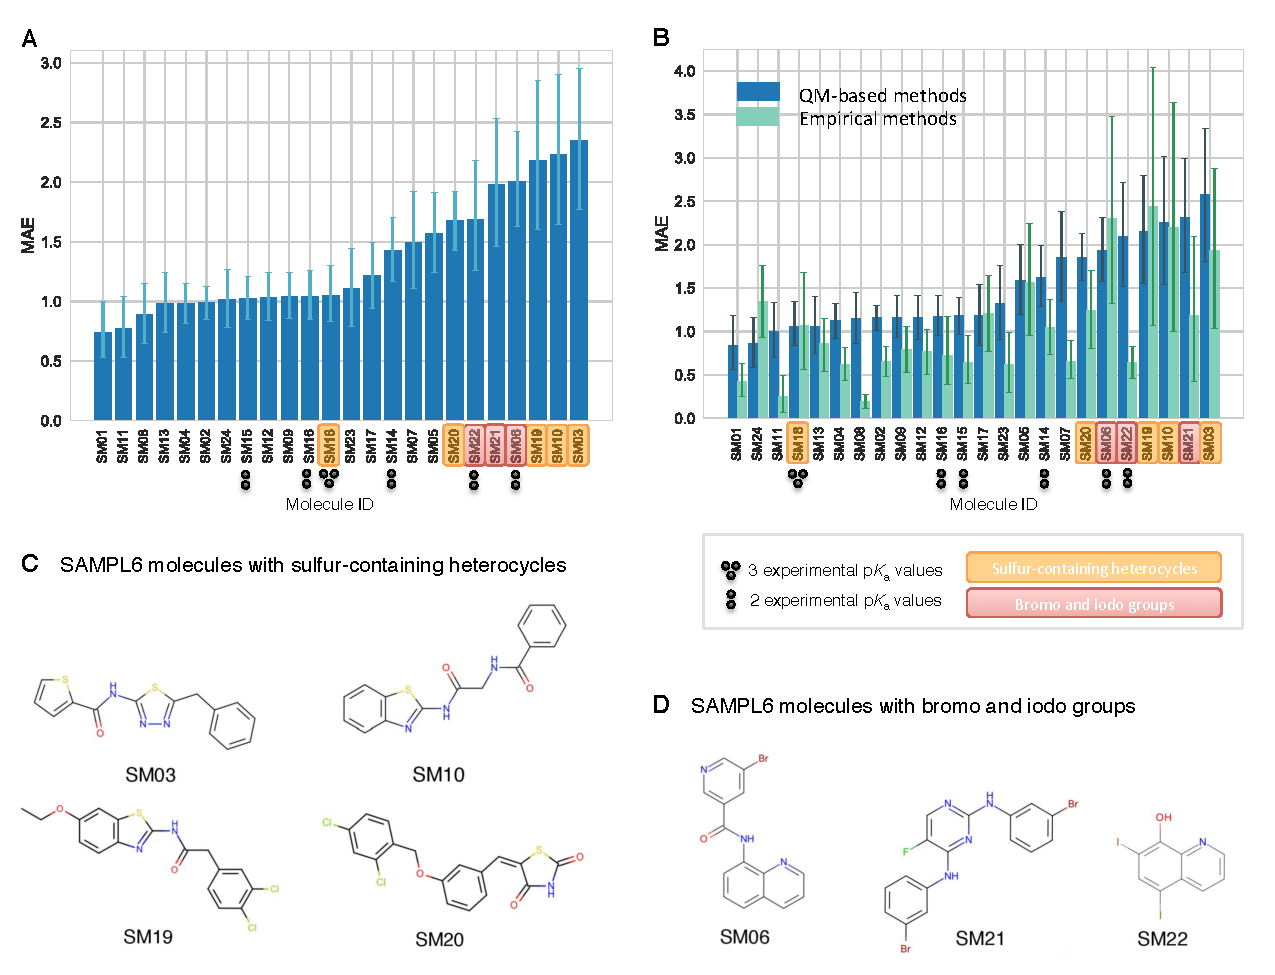
\includegraphics[width=1.0\linewidth]{figures/typeIII_molecular_MAE_fig.pdf}
\caption{{\bf Average prediction accuracy calculated over all prediction methods was lower for molecules with sulfur-containing heterocycles, bromo, and iodo groups.}
{\bf(A)} MAE calculated for each molecule as an average of all methods. {\bf(B)} MAE of each molecule broken out by method category. QM-based methods (blue) include QM predictions with or without linear empirical correction. Empirical methods (green) include QSAR, ML, DL, and LFER approaches. {\bf(C)} Depiction of SAMPL6 molecules with sulfur-containing heterocycles. {\bf(D)} Depiction of SAMPL6 molecules with iodo and bromo groups .
}
\label{fig:typeIII_molecular_MAE}
\end{figure}


\begin{figure}
\centering
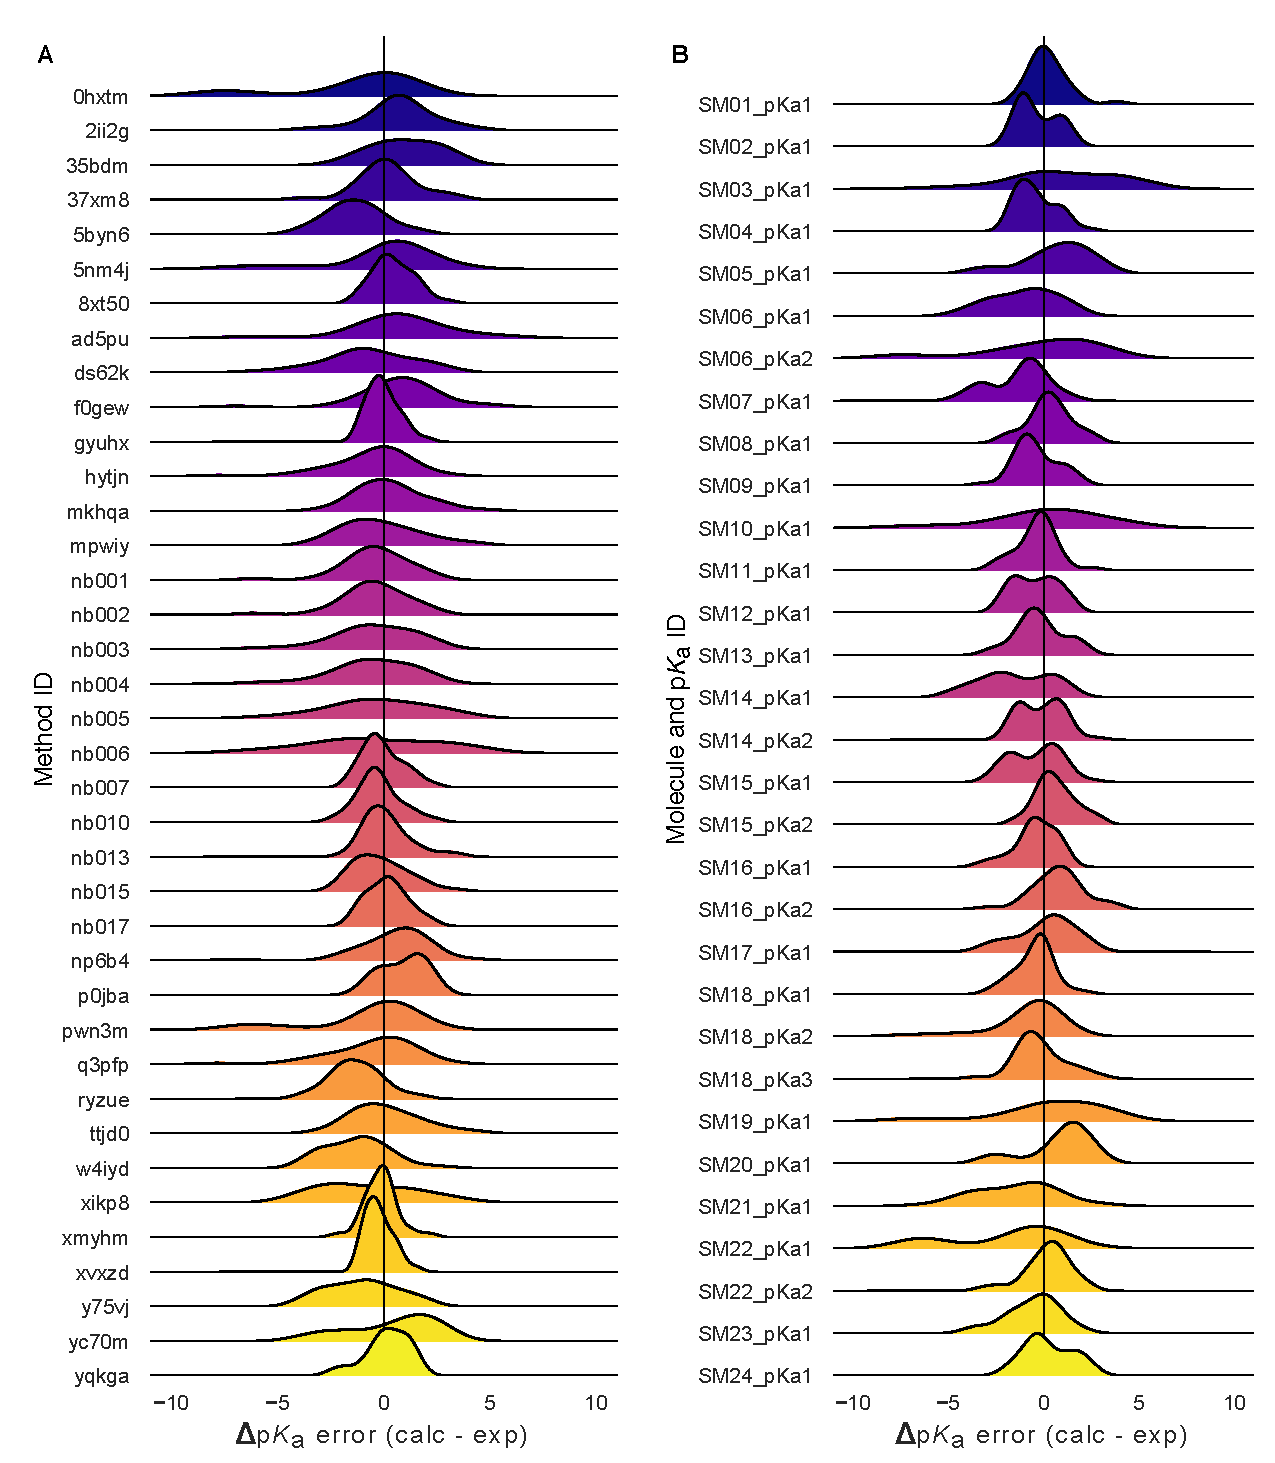
\includegraphics[width=0.8\linewidth]{figures/typeIII-error-distribution.pdf}
\caption{{\bf Macroscopic \pKa{} prediction error distribution plots show how prediction accuracy varies across methods and individual molecules.}
{\bf(A)} \pKa{} prediction error distribution for each submission for all molecules according to Hungarian matching. {\bf(B)} Error distribution for each SAMPL6 molecule for all prediction methods according to Hungarian matching. For multiprotic molecules, \pKa{} ID numbers (pKa1, pKa2, and pKa3) were assigned in the direction of increasing experimental \pKa{} value. 
}
\label{fig:typeIII-error-distribution}
\end{figure}

We have also looked for correlation with molecular descriptors for finding other potential explanations for why macroscopic \pKa{} predictions were larger in some molecules. 
While testing correlation between errors and many molecular descriptors it is important to keep the possibility of spurious correlations in mind. 
We haven't observed any significant correlation between numerical \pKa{} predictions and the descriptors we have tested. 
First of all, higher number of experimental \pKa{}s (Fig.~\ref{fig:typeIII_molecular_MAE}A) did not seem to associate with lower \pKa{} prediction performance. 
But we need to keep in mind that there was a low representation of multiprotic compounds in the SAMPL6 set (5 molecules with 2 macroscopic \pKa{}s and one molecule with 3 macroscopic \pKa{}).
Other descriptors we checked for were presence of amide groups, molecular weight, heavy atom count, rotatable bond count, heteroatom count, heteroatom to carbon ratio, ring system count, maximum ring size, and the number of microstates (as enumerated for the challenge). 
Correlation plots and R\textsuperscript{2} values can be seen in Fig.~\ref{fig:molecular_properties_vs_MAE_correlation}. 
We had suspected that \pKa{} prediction methods may be trained better for moderate values (4-10) than extreme values as molecules with extreme \pKa{}s are less likely to change ionization states close to physiological pH. To test this we look at the distribution of absolute errors calculated for all molecules and challenge predictions binned by experimental \pKa{} value 2 \pKa{} unit increments. 
As can be seen in Fig.~\ref{fig:macroscopic-pKa-error-vs-pKa-value}B, the value of true macroscopic \pKa{}s was not a factor affecting prediction error seen in SAMPL6 Challenge.


Fig.~\ref{fig:typeIII-error-distribution}B is helpful to answer the question of "Are there molecules with consistently overestimated or underestimated \pKa{}s?". This ridge plots shows the error distribution of each experimental \pKa{}. SM02\_pKa1, SM04\_pKa1, SM14\_pKa1, and SM21\_pKa1 were underestimated by majority of the prediction methods for more than 1 \pKa{} unit. 
SM03\_pKa1, SM06\_pKa2, SM19\_pKa1, and SM20\_pKa1 were overestimated by the majority of the preodction methods for more than 1 \pKa{} unit.
SM03\_pKa1, SM06\_pKa2, SM10\_pKa1, SM19\_pKa1, and SM22\_pKa1 have the highest spread of errors and were less accurately predicted overall. Refer to Ridge plots of Delta pKa error to identify compounds that were frequently mispredicted.




%%%
\subsection{Analysis of microscopic \pKa{} predictions using microstates determined by NMR for 8 molecules}

The common approach for analysing microscopic \pKa{} prediction accuracy has been to compare it to experimental macroscopic \pKa{} data, assuming experimental \pKa{}s describe titrations of distinguishable sides and, therefore, equal to microscopic \pKa{}s. But this typical approach fails to evaluate the methods in microscopic level.

Analysis of microscopic \pKa{} predictions of the SAMPL6 Challenge was not straight-forward due to lack of experimental data with microscopic detail. For 24 molecules macroscopic \pKa{}s were determined with spectrophotometric method. 
For 18 molecules single macroscopic titration was observed and for 6 molecules multiple experimental \pKa{}s were reported. 
For 18 molecules with single experimental \pKa{} it is probabable that the molecules are monoprotic and therefore macroscopic \pKa{} value is equal to the microscopic \pKa{}, but there is no direct experimental evidence to support that this is the case but only the support from prediction methods. 
There is always the possibility that the macroscopic \pKa{} observed is the result of two different titrations overlapping closely with respect to pH. 
We did not want to bias the blind challenge analysis with any prediction method. 
Therefore, we believe analyzing the microscopic \pKa{} predictions via Hungarian matching to experimental values with the assumption that the 18 molecules have single titratable site is not the best approach. 
Instead analysis at the level of macroscopic \pKa{}s is much more appropriate when a numerical matching scheme is the only option to evaluate predictions using macroscopic experimental data.

For a subset of the molecules in the dataset of 8 molecules, dominant microstates were inferred from NMR experiments. This dataset was extremely useful for guiding the assignment between experimental and predicted \pKa{} values based on microstates. In this section we present the performance evaluations of microscopic \pKa{} predictions for only the 8 compounds with experimentally determined dominant microstates.


\begin{figure}
\centering
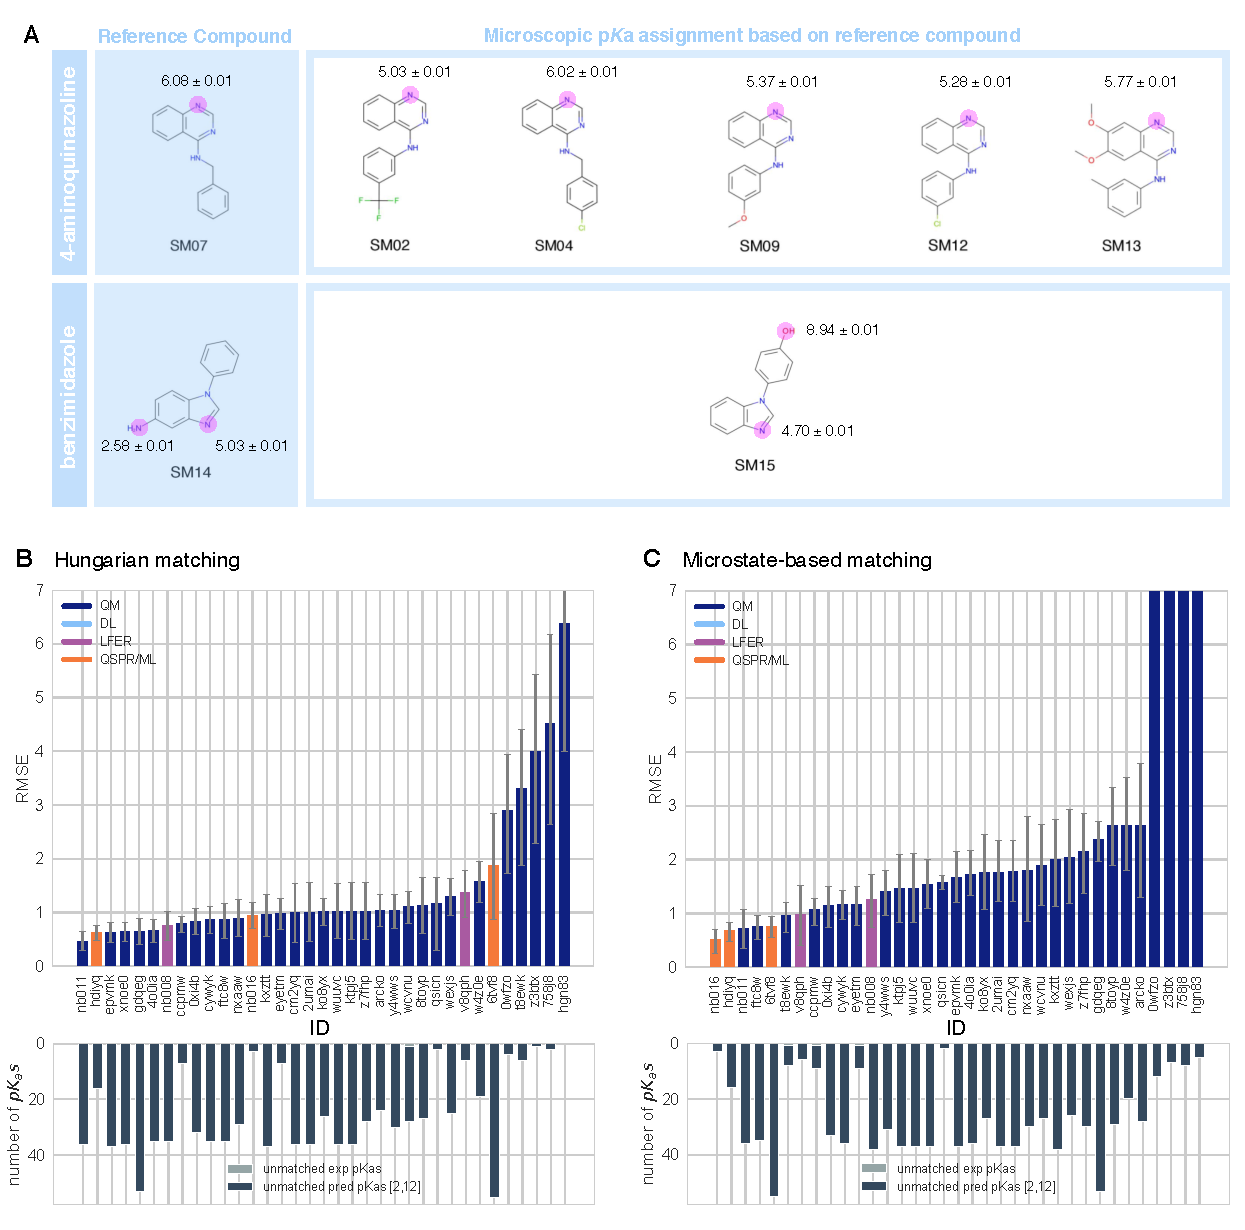
\includegraphics[width=1.0\linewidth]{figures/typeI_8_mol_matching_comparison.pdf}
\caption{{\bf NMR determination of dominant microstates allowed in depth evaluation of microscopic \pKa{} predictions of 8 compounds.} 
{\bf A} Dominant microstate sequence of two compounds (SM07 and SM14) were determined by NMR~\cite{Isik:2018:J.Comput.AidedMol.Des.}. Based on these reference compounds dominant microstates of 6 other derivative compounds were infered and experimental \pKa{} values were assigned to titratable groups with the assumption that only the dominant microstates have significant contributions to the experimentally observed \pKa{}.
{\bf B} RMSE vs. submission ID and unmatched \pKa{} vs. submission ID plots for the evaluation of microscopic \pKa{} predictions of 8 molecules by Hungarian matching to experimental macroscopic \pKa{}s. {\bf C} RMSE vs. submission ID and unmatched \pKa{} vs. submission ID plots showing the evaluation of microscopic \pKa{} predictions of 8 molecules by microstate-based matching between predicted microscopic \pKa{}s and experimental macroscopic \pKa{} values. Submissions \textit{0wfzo, z3btx, 758j8}, and \textit{hgn83} have RMSE values bigger than 10 \pKa{} units which are beyond the y-axis limits of subplot {\bf C} and {\bf B}.
RMSE is shown with error bars denoting 95\% confidence intervals obtained by bootstrapping over challenge molecules. Lower bar plots show the number of unmatched experimental \pKa{}s (light grey, missing predictions) and the number of unmatched \pKa{} predictions (dark grey, extra predictions) for each method between pH 2 and 12. Submission IDs are summarized in Table~\ref{submission-ID-table}. 
}
\label{fig:typeI-matching-algorithm-comparison}
\end{figure}


\subsubsection{Microstate-based matching revealed errors masked by \pKa{} value-based matching between experimental and predicted \pKa{}s}


Comparing microscopic \pKa{} predictions directly to macroscopic experimental \pKa{} values with numerical matching can lead to underestimation of errors. 
To demonstrate how numerical matching often masks the \pKa{} prediction errors we compared the performance analysis done by Hungarian matching to microstate-based matching for 8 molecules presented in Fig.~\ref{fig:typeI-matching-algorithm-comparison}A. RMSE calculated for microscopic \pKa{} predictions matched to experimental values via Hungarian matching is shown in Fig.~\ref{fig:typeI-matching-algorithm-comparison}B, while Fig.~\ref{fig:typeI-matching-algorithm-comparison}C shows RMSE calculated via microstate-based matching. 
What is important to notice is that the Hungarian matching leads to significantly lower RMSE compared to microstate-based matching. The reason is that the Hungarian matching assigns experimental \pKa{} values to predicted \pKa{} values only based on the closeness of the numerical values, without consideration of the relative population of microstates and microstate identities. 
Because of that a microscopic \pKa{} value that describes a transition between very low population microstates (high energy tautomers) can be assigned to the experimental \pKa{} if it has the closest \pKa{} value. 
This is not helpful, because in reality the microscopic \pKa{}s that influence the observable macroscopic \pKa{} the most are the ones with higher populations (transitions between low energy tautomers).

The number of unmatched predicted microscopic \pKa{s} are shown in lower bar plots of Fig.~\ref{fig:typeI-matching-algorithm-comparison}B and C, to emphasize the large number of microscopic \pKa{} predictions submitted by many methods. 
In the case of microscopic \pKa{} the number of unmatched predictions do not indicate an error in the form of an extra predicted \pKa{}, because the spectrophotometric experiments do not capture all microscopic \pKa{}s theoretically possible (transitions between all pairs of microstates that are 1 proton apart). 
\pKa{}s of transitions to and from very high energy tautomers are very hard to measure by experimental methods, including the most sensitive methods like NMR. 
The reason we plotted them was more to demonstrate how the increased number of prediction value choices for Hungarian matching can lead to erroneously low RMSE values. 
We have also checked how often Hungarian matching led to the correct matches between predicted and experimenal \pKa{} in terms of the microstate pairs, i.e. how often the microstate pair of the Hungarian match recapitulates the dominant microstate pair of the experiment. The overall accuracy of correct microstate pair match was found to be low for SAMPL6 Challenge submission. 
Fig.~\ref{fig:microstate-pairs-with-Hungarian-match-vs-experiments} shows that for most methods the predicted microstate pair selected by Hungarian match did not match experimentally determined microstate pair.
This means the lower RMSE results obtained from Hungarian matching are low for the wrong reason. 
Matching experimental and predicted values on the basis of microstate IDs do not suffer from this problem.  

The disadvantage of the evaluation through microstate-based matching approach is that the conclusions in this section are only about a subset of challenge compounds with limited diversity. This subset is composed of 6 molecules 4-aminoquinazoline and 2 molecules with benzimidazole scaffolds, and a total of 10 \pKa{} values. The sequence of dominant microstates for SM07 and SM14 were determined by NMR experiments directly~\citep{Isik:2018:J.Comput.AidedMol.Des.}, and dominant microstates of their derivatives were infered taking them as reference (Fig.~\ref{fig:typeI-matching-algorithm-comparison}). Although, we believe that microstate-based evaluation is more informative, the lack of a large experimental dataset limits the conclusions to a very narrow chemical diversity. 


\subsubsection{Accuracy of \pKa{} predictions evaluated by microstate-based matching}

\begin{figure}
\centering
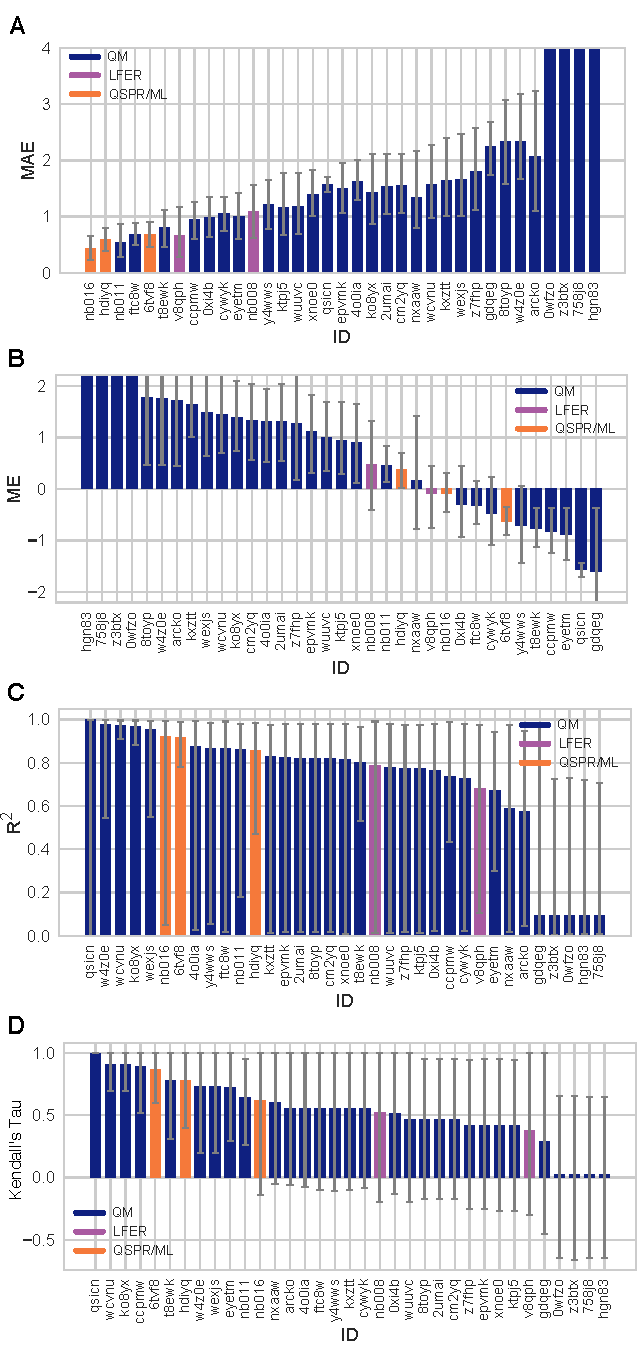
\includegraphics[width=0.5\linewidth]{figures/typeI_statistics.pdf}
\caption{{\bf Additional performance statistics for microscopic \pKa{} predictions for 8 molecules with experimentally determined dominant microstates.} 
Microstate-based matching was performed between experimental \pKa{} values and predicted microscopic \pKa{}s. 
Mean absolute error (MAE), mean error (ME), Pearson’s R\textsuperscript{2}, and Kendall’s Rank Correlation Coefficient Tau ($\tau$) are shown, with error bars denoting 95\% confidence intervals obtained by bootstrapping over challenge molecules. Methods are indicated by submission IDs. Submissions are colored by their method categories. Refer to Table~\ref{submission-ID-table} for submission IDs and method names. Submissions \textit{0wfzo, z3btx, 758j8}, and \textit{hgn83} have MAE and ME values bigger than 10 \pKa{} units which are beyond the y-axis limits of subplots {\bf A} and {\bf B}. A large number and wide variety of methods have a statistically indistinguishable performance based on correlation based statistic ({\bf C} and {\bf D}), in part because of the relatively small dynamic range the small size of the set of 8 molecules.
}
\label{fig:typeI-statistics}
\end{figure}

Both accuracy and correlation based statistics were calculated for predicted microscopic \pKa{} values after microstate-based matching. RMSE, MAE, ME, R\textsuperscript{2}, and Kendall's Tau results of each method are shown in Fig.~\ref{fig:typeI-matching-algorithm-comparison}C and Fig.~\ref{fig:typeI-statistics}. A table of the calculated statistics can be found in Table~\ref{SI-statistics-table-micro-pKa-8mol-microstate}. Due to small number of data points in this set, correlation based statistics calculated shows large uncertainty and provide less utility for distinguishing better performing methods. Therefore we focused more on accuracy based metrics for the analysis of microscopic \pKa{}s than correlation based metrics. In terms of accuracy of microscopic \pKa{} value, all three QSPR/ML based methods (\textit{nb016} (MoKa),\textit{hdiyq} (Simulations Plus), \textit{6tvf8} (OE Gaussian Process)), three QM-based methods (\textit{nb011} (Jaguar), \textit{ftc8w} (EC-RISM/MP2/cc-pVTZ-P2-q-noThiols-2par), \textit{t8ewk} (COSMOlogic\_FINE17)), and one LFER method (\textit{v8qph} (ACD/pKa GALAS)) achieved RMSE lower than 1 \pKa{} unit. The same 6 methods also have the lowest MAE.


\subsubsection{Evaluating microstate prediction accuracy of methods}

For many computational chemistry approaches including structure based modeling of protein-ligand interactions, predicting the ionization state and the exact position of protons is important to guide modeling.  
This is why in addition to being able to predict \pKa{} values accurately, we need \pKa{} prediction methods to be able to capture microscopic protonation states accurately. Even when the predicted \pKa{} value is very accurate, the predicted protonation site can be wrong. 
Therefore, we assessed if methods participating the SAMPL6 \pKa{} Challenge were predicting correctly the sequence of dominant microstates, i.e. dominant tautomers of each charge state observed between pH 2 and 12.


 Analyze which state has lowest free energy for each charge group ( The sequence of "experimentally visible states")
 
Dominant microstate prediction accuracy of microscopic \pKa{} prediction method are shown in Fig.~\ref{fig:typeI_dominant_microstate_accuracy}.
To extract the dominant tautomers predicted for the sequence of ionization states of each method, first, relative free energy of microstates were calculated at reference pH 0 ~\citep{Gunner:2020:J.Comput.AidedMol.Des.}. Then to determine dominant microstate of each charge, we have selected the lowest energy tautomer for each ionization states of the charges -1, 0, 1, and 2 (the charge range captured by NMR) experiments.
Than predicted and experimental dominant microstates were compared for each charge to calculate the fraction of correctly predicted dominant tautomers. This value is reported as the dominant microstate accuracy for all charges (Fig.~\ref{fig:typeI_dominant_microstate_accuracy}A). Dominant microsate prediction errors were present the methods participating in the SAMPL6 \pKa{} Challenge. 10 QM and 3 QSPR/ML methods did not make any mistakes in dominant microstate predictions, although, they are expected to  be making mistakes in the relative ratio of tautomers (free energy difference between microstates) as reflected by \pKa{} value errors. While all the participating QSPR/ML methods showed good performance in dominant microstate prediction, LFER and some QM methods made mistakes. Accuracy of the prediction of the neutral dominant tautomers was perfect for all methods, except \textit{qsicn} (Fig.~\ref{fig:typeI_dominant_microstate_accuracy}B). But errors in predicting the major tautomer of charge +1 was much more frequent. 22 out of 35 prediction sets made at least one error in prediction the lowest energy tautomer with +1 charge. We didn't include ionization states with charges -1 and +2 in this assessment because we had only one compound with these charges in the dataset. Never the less, dominant tautomer prediction errors seems to be a bigger problem for charged tautomers than the neutral tautomer.    

Experimental data of the sequence of dominant microstates was only available for 8 compounds. Therefore conclusions the performance of methods in terms of dominant tautomer prediction are limited to this narrow chemical diversity (benzimidazole and 4-aminoquinazoline derivatives). We present this analysis as a prototype of how microscopic \pKa{} predictions should be evaluated. To reach broad conclusions about which methods are better for capturing dominant microstates and ratios of tautomers we hope that in the future more extensive evaluations can be mode with larger experimental datasets following the strategy we are demonstrating here. Even if experimental microscopic \pKa{} measurement data is not available, experimental dominant tautomer determinations are still informative for assessing prediction methods.  

\begin{figure}[h!]
\centering
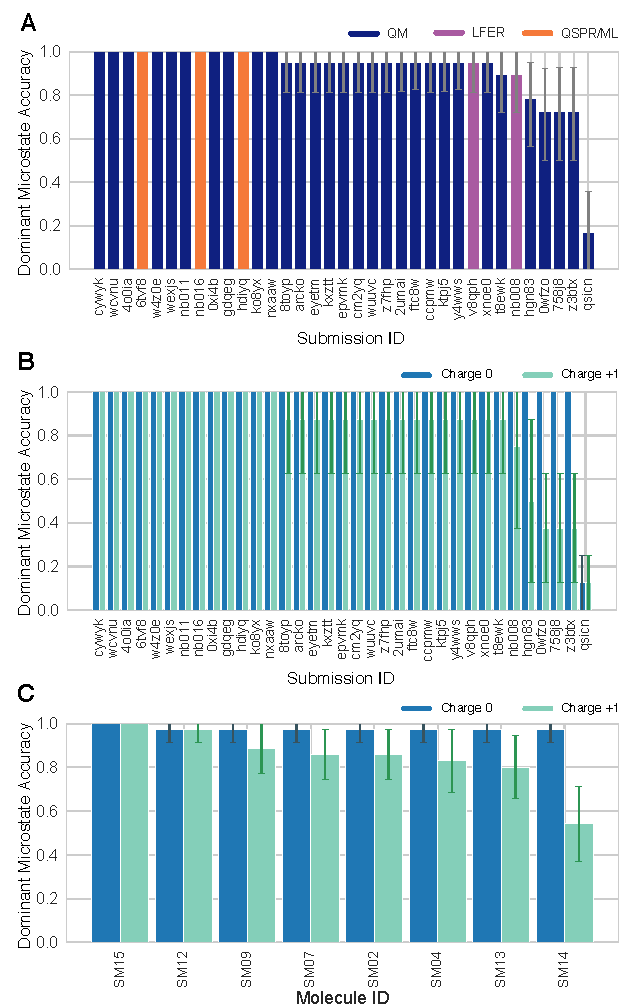
\includegraphics[width=0.5\linewidth]{figures/typeI_dominant_microstate_accuracy.pdf}
\caption{{\bf Some methods predicted the sequence of dominant tautomers inaccurately.} Prediction accuracy of dominant microstate of each charged state was calculated using the dominant microstate sequence determined by NMR for 8 molecules as reference. 
{\bf(A)} Dominant microstate accuracy vs. submission ID plot was calculated considering all the dominant microstates seen in the 8 molecule experimental microstate dataset. {\bf(B)} Dominant microstate accuracy vs. submission ID plot was generating considering only the dominant microstates of charge 0 and +1 seen in the 8 molecule experimental microstate dataset. Accuracy of each molecule is broken out by total charge of the microstate. {\bf(C)} Dominant microstate prediction accuracy calculated for each molecule averaged over all methods. In {\bf(B)} and {\bf(C)}, the accuracy of predicting the dominant neutral tautomer is showed in blue and the accuracy of predicting the dominant +1 charged tautomer is showed in green. Error bars denoting 95\% confidence intervals obtained by bootstrapping.
}
\label{fig:typeI_dominant_microstate_accuracy}
\end{figure}

Focusing on dominant microstate sequence prediction accuracy from the perspective of molecules showed that major tautomer of SM14 cationic form was the most frequently mispredicted one. 
Fig.~\ref{fig:typeI_dominant_microstate_accuracy} shows the dominant microstate prediction accuracy calculated for individual molecules for charge states 0 and +1, averaged over all prediction methods. 
SM14, the molecule that exibits highest microstate prediction error, has two experimental \pKa{} values that were 2.4 \pKa{} units apart and we suspect that could be a contributor to the difficulty of predicting microstates accurately. 
Other molecules are monoprotic (4-aminoquinazolines) or their experimental \pKa{} values are very well separated (SM14, 4.2 \pKa{} units). 
It would be very interesting to expand this assessment to a larger variety of drug-like molecules to discover for which structures tautomer predictions are more accurate and for which structure computational predictions are not as reliable.


\subsubsection{Consistently-well performing methods for microscopic \pKa{} predictions}

To determine consistently top-performing methods for microscopic \pKa{} predictions we have determined different criteria than macroscopic \pKa{} predictions: having perfect dominant microstate prediction accuracy, unmatched \pKa{} count of 0, and ranking in the top 10 according RMSE and MAE. Correlation based statistics were not fount to have utility for discriminating performance due to large uncertainties in this statistics for a small dataset of 10 \pKa{} values. Unmatched predicted \pKa{} count was also not a consideration, since experimental data was only informative for the \pKa{} between dominant microstates and did not capture the all possible theoretical transitions between microstate pairs. Table~\ref{typeI-well-performing-methods-table} reports six methods that have consistent well performance according to many metrics, although evaluated only for the 8 molecule set due to limitations of the experimental dataset. Six methods were divided evenly between methods of QSPR/ML category and QM category. \textit{nb016} (MoKa), \textit{hdiyq} (Simulations Plus), and \textit{6tvf8} (OE Gaussian Process) were QSPR and ML based methods that performed well. \textit{nb011} (Jaguar), \textit{0xi4b}(EC-RISM/B3LYP/6-311+G(d,p)-P2-phi-noThiols-2par), and \textit{cywyk} (EC-RISM/B3LYP/6-311+G(d,p)-P2-phi-noThiols-2par) were QM predictions with linear empirical corrections with good performance with microscopic \pKa{} predictions. 

Simulations Plus \pKa{} prediction method is the only method that appeared to be consistently well performing in both the assessment for macroscopic and microscopic \pKa{} prediction (\textit{gyuhx} and \textit{hdiyq}). However it is worth noting that two methods that were in consistently top-performing methods list for macroscopic \pKa{} predictions lacked equivalent submissions of their underlying microscopic \pKa{} predictions and therefore could not be evaluated at the microstate level. These methods were \textit{} (ACD/Classic pKa) and \textit{xvxzd}(DSD-BLYP-D3(BJ)/def2-TZVPD//PBEh-3c[DCOSMO-RS] + RRHO(GFN-xTB[GBSA]) + Gsolv(COSMO-RS[TZVPD]) and linear fit). 






\begin{table}[h]
\begin{center}
\begin{threeparttable}
\centering\scriptsize
\caption{{\bf Top performing methods for microscopic \pKa{} predictions based on consistent ranking within the Top~10 according to various statistical metrics calculated for 8 molecule dataset.} 
Performance statistics are provided as mean and 95\% confidence intervals. Submissions that rank in the Top~10 according to RMSE and MAE, and have perfect dominant microstate prediction accuracy were selected as consistently well-performing methods. Correlation-based statistics (R\textsuperscript{2}, and Kendall's Tau), although reported in the table, were excluded from the statistics used for determining top-performing methods. This was because correlation-based statistics were not very discriminating due to narrow dynamic range and the small number of data points in the 8 molecule dataset with NMR-determined dominant microstates. 
} 
\label{typeI-well-performing-methods-table}
\begin{tabular}{@{}lllllllll@{}}
\toprule
\textbf{\begin{tabular}[c]{@{}l@{}}Submission\\ ID\end{tabular}} & \textbf{Method Name} & \textbf{\begin{tabular}[c]{@{}l@{}}Dominant \\ Microstate \\ Accuracy\end{tabular}} & \textbf{RMSE} & \textbf{MAE} & \textbf{R\textsuperscript{2}} & \textbf{Kendall's Tau} & \textbf{\begin{tabular}[c]{@{}l@{}}Unmatched \\ Exp. \pKa{} \\ Count\end{tabular}} & \textbf{\begin{tabular}[c]{@{}l@{}}Unmatched \\ Pred. \pKa{} \\ Count [2,12]\end{tabular}} \\ \midrule
\rowcolor[HTML]{EFEFEF} 
{\color[HTML]{000000} \textit{nb016}} & {\color[HTML]{000000} MoKa} & {\color[HTML]{000000} 1.0 [1.0, 1.0]} & {\color[HTML]{000000} 0.52 [0.25, 0.71]} & {\color[HTML]{000000} 0.43 [0.23, 0.65]} & {\color[HTML]{000000} 0.92 [0.05, 0.99]} & {\color[HTML]{000000} 0.62 [-0.14, 1.00]} & {\color[HTML]{000000} 0} & {\color[HTML]{000000} 3} \\
\textit{hdiyq} & S+pKa & 1.0 [1.0, 1.0] & 0.68 [0.49, 0.83] & 0.60 [0.39, 0.80] & 0.86 [0.47, 0.98] & 0.78 [0.40, 1.00] & 0 & 16 \\
\rowcolor[HTML]{EFEFEF} 
\textit{nb011} & Jaguar & 1.0 [1.0, 1.0] & 0.72 [0.35, 1.07] & 0.54 [0.28, 0.86] & 0.86 [0.18, 0.98] & 0.64 [0.26, 0.95] & 0 & 36 \\
\textit{6tvf8} & OE Gaussian Process & 1.0 [1.0, 1.0] & 0.76 [0.55, 0.95] & 0.68 [0.46, 0.90] & 0.92 [0.78, 0.99] & 0.87 [0.6, 1.00] & 0 & 55 \\
\rowcolor[HTML]{EFEFEF} 
\textit{0xi4b} & \begin{tabular}[c]{@{}l@{}}EC-RISM/B3LYP/6-311+G(d,p)\\ -P3NI-phi-noThiols-2par\end{tabular} & 1.0 [1.0, 1.0] & 1.15 [0.75, 1.50] & 0.98 [0.63, 1.36] & 0.77 [0.02, 0.98] & 0.51 [-0.14, 1.00] & 0 & 33 \\
\textit{cywyk} & \begin{tabular}[c]{@{}l@{}}EC-RISM/B3LYP/6-311+G(d,p)\\ -P2-phi-noThiols-2par\end{tabular} & 1.0 [1.0, 1.0] & 1.17 [0.88, 1.41] & 1.06 [0.74, 1.35] & 0.73 [0.02, 0.98] & 0.56 [-0.08, 1.00] & 0 & 36 \\ \bottomrule
\end{tabular}
\end{threeparttable}
\end{center}
\end{table}



%%%
\subsection{How do \pKa{} prediction errors impact protein-ligand binding affinity predictions?}

Physical modeling methods for predicting protein-ligand binding affinities rely on \pKa{} predictions for modeling the protein and the ligand. As SAMPL6 \pKa{} Challenge only focused on small molecule \pKa{} prediction we will ignore the protonation state effects of the protein for now.
Many affinity prediction methods such as docking,  MM/PBSA, MM/GBSA, absolute or alchemical relative free energy calculation methods predict the affinity of a fixed protonation state of the ligand to a receptor.
These models strictly depend on \pKa{} predictions for determining possible protonation states of the ligand in aqueous environment and in protein complex, as well as the free energy penalty to reach those states~\citep{deOliveira:2019:J.Chem.TheoryComput.}. Accuracy of \pKa{} predictions can become a limitation for the performance of physical models that try to capture molecular association.

In terms of the ligand protonation states, there are two ways in which the \pKa{} prediction errors can influence the prediction accuracy for protein-ligand binding free energies as depicted in Fig.~\ref{fig:pKa-effects-on-protein-ligand-binding}. First scenario is when ligand is present in aqueous solution in multiple protonation states (Fig.~\ref{fig:pKa-effects-on-protein-ligand-binding}A).
When only the minor aqueous protonation state contributes to protein-ligand complex formation, overall binding free energy ($\Delta G_{bind}$) needs to be calculated as the sum of binding affinity of the minor state and the protonation penalty of that state ($\Delta G_{prot}$). 
$\Delta G_{prot}$ is a function of pH and \pKa{}.
A 1 unit of error in \pKa{} value would lead to 1.36 kcal/mol error in overall binding affinity, if the protonation state with the minor population binds the protein. 
The equations in Fig.~\ref{fig:pKa-effects-on-protein-ligand-binding}A show the calculation of overall affinity.

%\begin{equation}
%\Delta G_{bind} =\Delta G_{bind}^{C} + \Delta G_{prot}
%\end{equation}

%\begin{equation}
%\Delta G_{bind} =\Delta G_{bind}^{C} + RT(pH - pK_a) \ln{(10)}
%\end{equation}

In addition to multiple protonation states being present in the aqueous environment, multiple charge states can contribute to complex formation (Fig.~\ref{fig:pKa-effects-on-protein-ligand-binding}B). Then, overall free energy of binding needs to include a Multiple Protonation States Correction (MPSC) term ($\Delta G_{corr}$). MPSC is a function of pH, aqueous \pKa{} of the ligand, and the difference between the binding free energy of charged and neutral species ($\Delta G_{bind}^{C} - \Delta G_{bind}^{N}$) as shown in Fig.~\ref{fig:pKa-effects-on-protein-ligand-binding}B.

%\begin{equation}
%\Delta G_{bind} =\Delta G_{bind}^{N} + \Delta G_{corr}
%\end{equation}

%\begin{equation}
%\Delta G_{bind} =\Delta G_{bind}^{N} - RT\ln{\frac{1 + e^{-\frac{\Delta G_{bind}^{C} - \Delta G_{bind}^{N}}{RT}}10^{pK_a - pH}}{1 + 10^{pK_a - pH}}}
%\end{equation}

\begin{figure}[h]
\centering
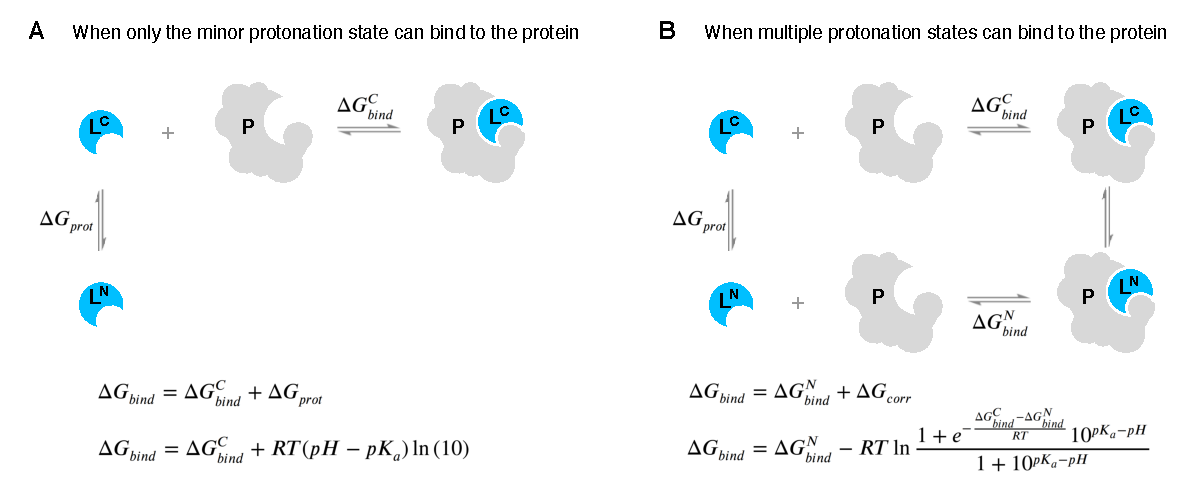
\includegraphics[width=1.0\linewidth]{figures/pKa-effects-on-protein-ligand-binding.pdf}
\caption{ {\bf Aqueous \pKa{} of the ligand can influence overall protein-ligand binding affinity.} {\bf A} When only the minor aqueous protonation state contributes to protein-ligand complex formation, overall binding free energy ($\Delta G_{bind}$) needs to be calculated as the sum of binding affinity of the minor state and the protonation penalty of that state. {\bf B} When multiple charge states contribute to complex formation, overall free energy of binding includes a multiple protonation states correction (MPSC) term ($\Delta G_{corr}$). MPSC is a function of pH, aqueous \pKa{} of the ligand, and the difference between the binding free energy of charged and neutral species ($\Delta G_{bind}^{C} - \Delta G_{bind}^{N}$).
}
\label{fig:pKa-effects-on-protein-ligand-binding}
\end{figure}

Using Equation 9 we can model the true MPSC ($\Delta G_{corr}$) value with respect to the difference between pH and the \pKa{} of the ligand, to see when this value has significant impact to overall binding free energy. In Fig.~\ref{fig:pKa-inaccuracy-and-MPSC}, true MPSC value that needs to be added to the $\Delta G_{bind}^{N}$ is shown for ligands with varying binding affinity difference between protonation states ($\Delta\Delta G = \Delta G_{bind}^{C} - \Delta G_{bind}^{N}$) and varying free energy of binding difference between the protonation states. Fig.~\ref{fig:pKa-inaccuracy-and-MPSC}A shows the simulation of a case where for a monoprotic base which has a charged state with lower affinity than the neutral state. Solid lines show the true correction. In situations where \pKa{} is lower than pH, correction factor disappears as the ligand fully populates the neutral state ($\Delta G_{bind} = \Delta G_{bind}^{N}$). As the \pKa{} value gets larger than the pH, the charged state is populated more and $\Delta G_{corr}$ value increases to approach  significant $\Delta\Delta G$. 
What is interesting to note is the pH-\pKa{} range that $\Delta G_{corr}$ changes.
It is often assumed that for a basic ligand if \pKa{} of a ligand is more than 2 units higher than the pH, then only 1\% of the population is in neutral state and it is safe to approximate the overall binding affinity with $\Delta G_{bind}^{C}$ only. Based on the relative free energy difference between ligand this assumption is not always correct. As seen in Fig.~\ref{fig:pKa-inaccuracy-and-MPSC}A, responsive region of $\Delta G_{corr}$ can span 3 pH units for a system with $\Delta\Delta G = 1 kcal/mol$  or 5 pH units for a system with $\Delta\Delta G = 4 kcal/mol$. This highlights that the range of \pKa{} values that impact binding affinity predictions is wider than previously appreciated. Molecules with \pKa{}s several units away from the physiological pH can still impact the overall binding affinity significantly due to MPSC. 

Despite the need to capture the contributions of multiple protonations states by including MPSC in binding affinity calculations, inaccurate \pKa{} predictions can lead to errors in $\Delta G_{corr}$  and overall free energy of binding prediction. In Fig.~\ref{fig:pKa-inaccuracy-and-MPSC}A dashed lines show predicted $\Delta G_{corr}$ based on \pKa{} error of -1 units. We have chosen a \pKa{} error of 1 units as this is the average performance expected from the \pKa{} prediction methods based on the SAMPL6 Challenge. Underestimated \pKa{} causes underestimated $\Delta G_{corr}$ and overestimated affinities for a varying range of pH - \pKa{} values depending on binding affinity difference between protonation states($\Delta\Delta G$).
In Fig.~\ref{fig:pKa-inaccuracy-and-MPSC}B dashed lines shows how the magnitude of the absolute error caused by calculating $\Delta G_{corr}$ with an inaccurate \pKa{} varies with respect to pH. Different colored lines show simulated results with varying binding affinity difference between protonation states. For a system whose charged state has lower affinity than the neutral state ($\Delta\Delta G$ = 2 kcal/mol), the absolute error caused by underestimated \pKa{} by 1 units only can be up to 0.9 kcal/mol.
For a system whose charged state has even lower affinity than the neutral state ($\Delta\Delta G$ = 4 kcal/mol), the absolute error caused by underestimated \pKa{} by 1 units only can be up to 1.2 kcal/mol.
The magnitude of errors contributing to overall binding affinity are too large to be neglected. Improving the accuracy of small molecule \pKa{} prediction methods can help to minimize the error in predicted MPSC.

With the current level of \pKa{} prediction accuracy as observed in SAMPL6 Challenge, is it advantageous to include MPSC in affinity predictions that may be include errors caused by \pKa{} predictions? We provide a comparison of the two choices to answer this question: (1) Neglecting MPSC completely and assuming overall binding affinity is captured by $\Delta G_{bind}^{N}$, (2) including MPSC with potential error in overall affinity calculation. The magnitude of error caused by Choice 1 (ignoring MPSC) is depicted as solid line in Fig.~\ref{fig:pKa-inaccuracy-and-MPSC}B and the magnitude of error caused by MPSC computed with inaccurate \pKa{}  is depicted as dashed lines. What is the best strategy? Error due to choice 1 is always larger than error due to choice 2 for all pH-\pKa{} values. In this scenario including MPSC improves overall binding affinity prediction. The error caused my inaccurate \pKa{} is smaller than the error caused by neglecting MPSC. 

The same question about whether or not an MPSC calculated based on an inaccurate \pKa{} should be included in binding affinity predictions can be asked for different circumstances underestimated or overestimated \pKa{} values, charged states with higher or lower affinities than the neutral states. We tried to capture these 4 circumstances in four quadrants of Fig.~\ref{fig:pKa-inaccuracy-and-MPSC}. In the case of overestimated \pKa{} values (Fig.~\ref{fig:pKa-inaccuracy-and-MPSC}E-H) it can be seen that for the most of the pH-\pKa{} range it is more advantageous to include the predicted MPSC in affinity calculations, except a smaller window where the opposite choice would be more advantegious. For instance, for the system with $\Delta\Delta G$ = 2 kcal/mol and overestimated \pKa{} (Fig.~\ref{fig:pKa-inaccuracy-and-MPSC}E) for the pH-\pKa{} region between -0.5 and 2, including predicted $\Delta G_{corr}$ causes more error than ignoring MPSC. 

In reality we do not know the exact magnitude or the direction of the error of our predicted \pKa{}, therefore using simulated MPSC error plots to make the decision about when to include MPSC in binding affinity predictions is not possible. But based on the analysis of extreme cases, with 1 unit of \pKa{} error including MPSC correction is more often than not helpful in imporving binding affinity predictions. The detrimental effect of \pKa{} inaccuracy is still significant, however, future improvements in \pKa{} prediction methods can improve the accuracy of MPSC and binding affinity predictions of ligands which have multiple protonation states that contribute to aqueous or complex populations. Achieving \pKa{} value prediction accuracy of 0.5 units would significantly help the binding affinity models to incorporate more accurate MPSC terms.   



\begin{figure}
\centering
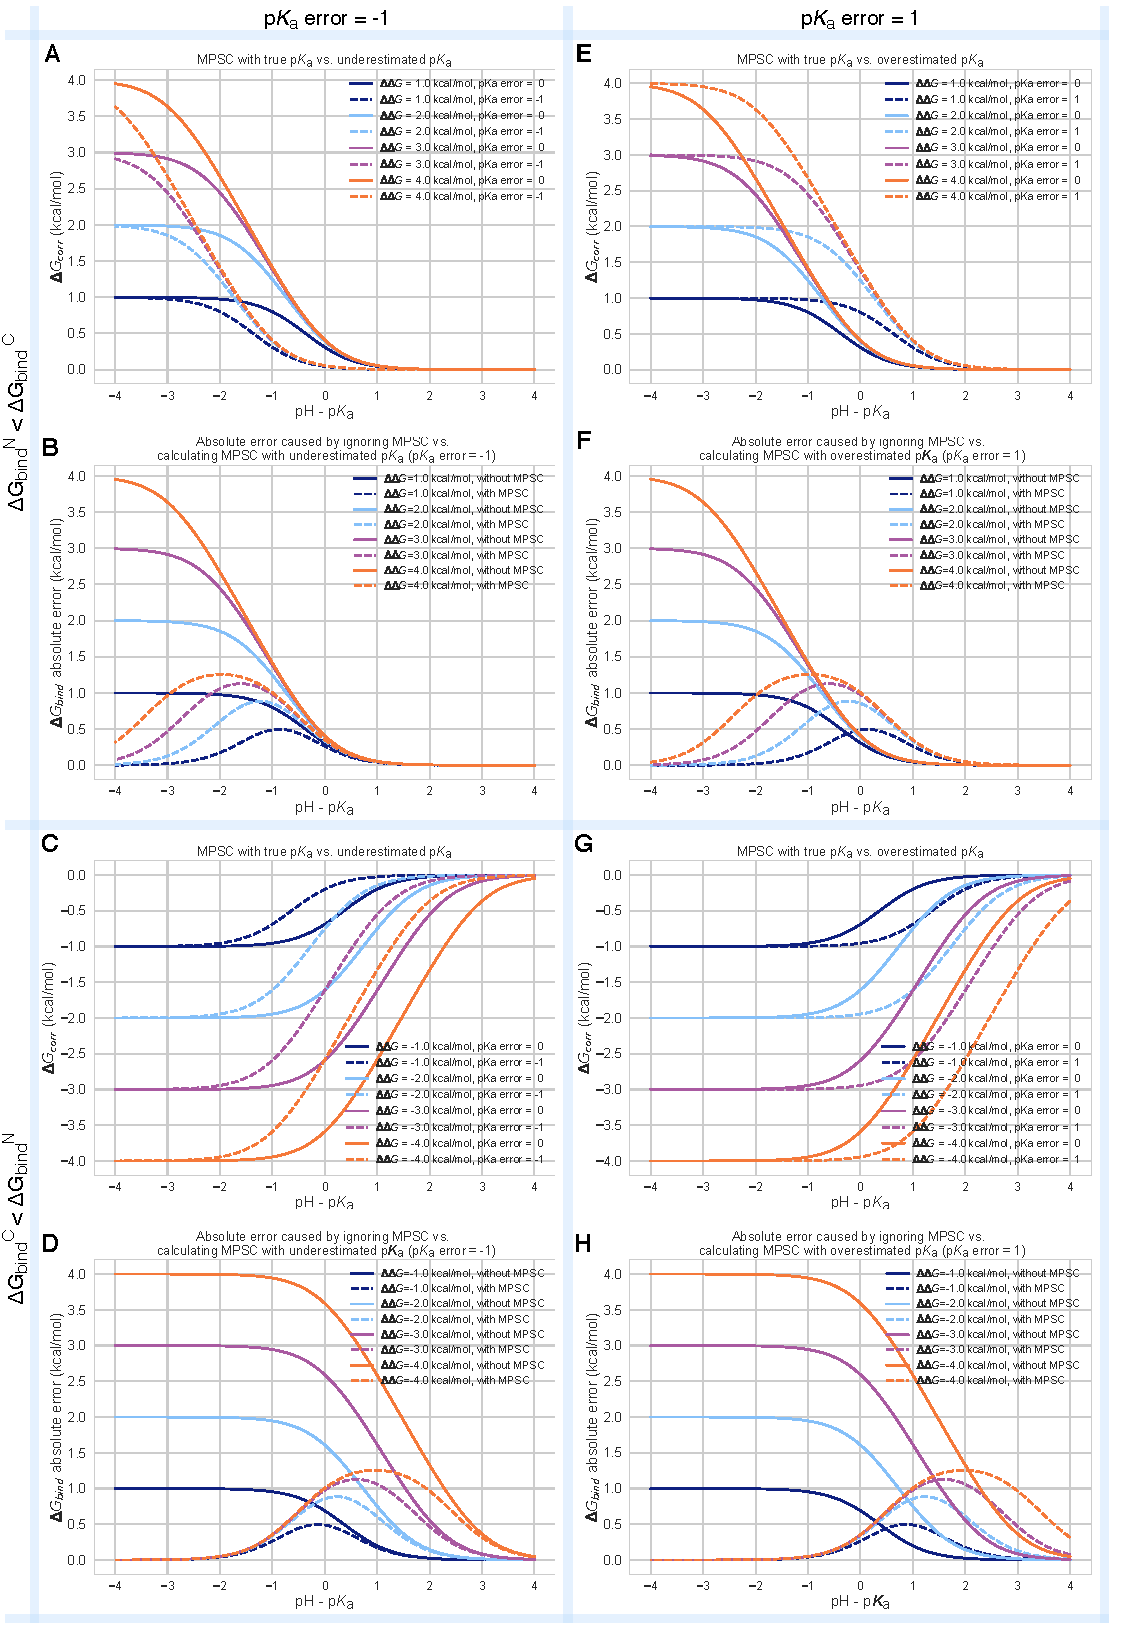
\includegraphics[width=0.8\linewidth]{figures/pKa-inaccuracy-and-MPSC.pdf}
\caption{ {\bf Inaccuracy of \pKa{} prediction ($\pm$ 1 unit) affects the the accuracy of MPSC and overall protein-ligand binding free energy calculation in varying amounts based on aqueous \pKa{} value and relative binding affinity of individual protonation states ($\Delta\Delta G = \Delta G_{bind}^{C} - \Delta G_{bind}^{N}$).} 
All calculations are made for 25\degree C, and for a ligand with single basic titratable group. {\bf A, C, E, and G} show MPSC ($\Delta G_{corr}$) calculated with true vs. inaccurate \pKa{}. {\bf B, D, F, and H} show comparison of the absolute error to $\Delta G_{bind}$ caused by ignoring the MPSC completely (solid lines) vs. calculating MPSC based in inaccurate \pKa{} value (dashed lines). These plots provide guidence on when it is beneficial to include MPSC correction based on \pKa{} error, pH - \pKa{}, and $\Delta\Delta G$. 
}
\label{fig:pKa-inaccuracy-and-MPSC}
\end{figure}



%%%
\subsection{Take-away lessons from SAMPL6 \pKa{} Challenge}

SAMPL6 \pKa{} Challenge showed that in general \pKa{} prediction performance of computational methods are lower than expected for drug-like molecules.   
Multiple titration sutes, tautomerization, frequent presence of heterocycles and extended conjugation patterns, as well as high number of rotatable bonds, and the possibility of intramolecular hydrogen bonds are factors that complicate \pKa{} prediction of drug-like molecules.
For macroscopic \pKa{} predictions have not yet reached experimental accuracy. 
Inter-method variability of macroscopic \pKa{} measurements can be around 0.5 \pKa{} units~\citep{Fraczkiewicz:2013:ReferenceModuleinChemistryMolecularSciencesandChemicalEngineering}. 
There was not a single method in SAMPL6 Challenge that achieved RMSE around 0.5 or lower for macropscopic \pKa{} predictions for the 24 molecule set of kinase inhibitor fragment-like molecules.
Lower RMSE values were observed in the microscopic \pKa{} evaluation section of this study for some methods however the 8 molecule set used for that analysis poses a very limited dataset to reach conclusions about general expectations for drug-like molecules.

As the majority of experimental data was in the form of macroscopic \pKa{} values, we had to adopt a numerical matching algorithm (Hungarian matching) to pair predicted and experimental values to calculate performance statistics of macroscopic \pKa{} predictions. Accuracy, correlation, and extra/missing \pKa{} prediction counts were the main metrics for macroscopic \pKa{} evaluations. An RMSE range of 0.7 to 3.2 \pKa{} units.
Only five methods achieved RMSE between 0.7-1 \pKa{} units, while an RMSE between 1.5-3 log units was observed for the majority of methods. All four methods of LFER category and three out of 5 QSPR/ML methods achieved RMSE less than 1.5 \pKa{} units. All the QM methods that achieved this level of performance included linear empirical corrections to rescale and unbias their \pKa{} predictions. 

Based on consideration of multiple error metrics, we compiled a short list of consistently-well performing methods for macroscopic \pKa{} evaluations. Two methods from QM+LEC methods, one QSPR/ML, two empricial methods achieved consistent performance according to many metrics. The common features of the two empirical methods were their large training sets (16000-17000 compounds) and being commercial prediction models.

There were four submissions of QM-based methods that utilized COSMO-RS implicit solvation model. 
It was interesting that while three of these achieved the lowest RMSE among QM-based methods (\textit{xvxzd}, \textit{yqkga}, and \textit{8xt50})~\citep{Pracht:2018:J.Comput.AidedMol.Des.} and one of them showed the highest RMSE (\textit{0hxtm} (COSMOtherm\_FINE17)) in SAMPL6 Challenge macroscopic \pKa{} predictions. Comparison of these methods indicates that capturing conformational ensemble of microstates, high level QM calculations, and RRHO corrections were factors contributing to better macroscopic \pKa{} predictions.
Linear empirical corrections applied QM calculations imporved results, especially when the linear correction is calibrated for an experimental dataset using the same level of theory  ast the deprotonation free energy predictions (as in \textit{xvxzd}).
This challenge also points to the advantage of COSMO-RS solvation approach compared to other implicit solvent models.

Evaluation of macroscopic \pKa{} prediction accuracy of individual molecules on average considering all the predictions in SAMPL6 Challenge provided insight into which molecules posed greater difficulty for \pKa{} predictions.    \pKa{} prediction errors were higher for compounds with sulfur-containing heterocyles, iodo, and bromo groups. This trend was also conserved when only QM-based methods were analyzed. SAMPL6 \pKa{} dataset consisted of only 24 small molecules which limited our ability to statistically confirm this conclusion, however, we believe it is worth reporting molecular features that coincided with larger errors even if we can not evaluate the driving reason for these failures. 

Utilizing a numerical matching algorithm to pair experimental and predicted macroscopic \pKa{} values was a necessity, however, this approach did not capture all aspects of prediction errors. Computing the number of missing or extra \pKa{} predictions remaining after Hungarian matching, provided a window of observing macroscopic \pKa{} prediction errors such as number of macroscopic transitions or ionization states expected in a pH interval. In \pKa{} evaluation studies it is very typical to just focus on \pKa{} value errors evaluated after matching, and to ignore \pKa{} prediction errors that the matching protocol can not capture. SAMPL6 \pKa{} Challenge results showed sporatic presence of missing \pKa{} predictions and very frequent case of extra \pKa{} predictions. Both indicates failures to capture the correct sequence of ionizations states. The traditional way of evaluating \pKa{}s that only focuses on the \pKa{} value error after some sort of numerical match between predictions and experimental values may have motivated these types of errors as there would be no penalty for missing a macroscopic deprotonation and predicting an extra one. This problem does not seem to be specific to any method category.

We have used the 8 molecule subset of SAMPL6 compounds with NMR-based dominant microstate sequence information to demonstrate the advantage of evaluating \pKa{} prediction on the level of microstates.
Comparison of statistics computed by Hungarian matching and microstate-based matching on 8 molecule dataset showed how Hungarian matching, despite being the optimal matching algorithm, can mask errors in \pKa{} predictions. 
Errors computed by microstate-based matching were larger compared to numerical matching algorithms in terms of RMSE.
Microscopic \pKa{} analysis with numerical matching algorithms may mask errors due to higher number of guesses made.
Numerical matching based on \pKa{} values also ignores information regarding the relative population of states. Therefore, it can lead to \pKa{}s defined between very low energy microstate pairs to be matched to the experimentally observable \pKa{} between microstates of higher populations. 
Of course the predicted \pKa{} value could be correct however the predicted microstates would be wrong. Such mistakes caused by Hungarian matching were observed frequently in SAMPL6 results and therefore we decided microstate-based matching of \pKa values provides a more realistic picture of method performance.  

Analysis of dominant microstate prediction accuracy of microscopic \pKa{} showed that some QM and LFER methods made mistakes in predicting the dominant tautomers of the ionization states seen experimentaly. Dominant tautomer prediction seemed to be a more prominant problem for charged tautomers than the neutral tautomer. The easiest way to extract dominant microstate sequence from predictions is to calculate relative free energy of microstates at any reference pH, and determining the lowest energy state in each ionization state. Errors in dominant microstate predictions was very rare for neutral tautomers, but more frequent in cationic tautomers with +1 charge of the 8 molecule set. SM14 was the molecule with the lowest dominant microstate prediction accuracy, while dominant microstates predictions for SM15 were perfect for all molecules. SM14 and SM15 both have two experimental \pKa{}s and benzimidazole scaffold. The difference between them is the distance between the experimental \pKa{} values which is smaller for SM14. This results makes sense from the perspective of relative free energies of microstates. Closer \pKa{} values mean that the free energy difference between different microstates are smaller for SM14, and therefore any error in predicting the relative free energy of tautomers is more likely to cause reordering of relative populations of microstates and impact the accuracy of dominant microstate predictions. 
It would have been extremely informative to evaluate the tautomeric ratios and relative free energy predictions of microstates, however, experimental data was missing for this approach.

According to statistics calculated with microstate-based matching, we determined a shortlist of consistently well-performing methods for microscopic \pKa{} predictions of 8 molecule set. These methods that ranked in top 10 according to RMSE, MEA, and had perfect dominant microstate prediction accuracy included three methods from QM+LEC category and three from QSPR/ML category. Simulations Plus \pKa{} prediction method was the only method that appeared to be consistently well performing in both the assessment for macroscopic and microscopic \pKa{} prediction (\textit{gyuhx} and \textit{hdiyq}), although, due to the size of the experimental datasets evaluation of macroscopic \pKa{} prediction carried more weight in this performance assessment. Still microscopic \pKa{} evaluation can provide much more in depth analysis and can be more informative about capturing reasons for failure.

The performance levels of microscopic and macroscopic \pKa{} prediction as seen in SAMPL6 \pKa{} Challenge assessment can be detrimental to the accuracy of protein-ligand affinity predictions and other pH-dependent physicochemical property predictions such as distribution coefficients, membrane permeability, and solubility.
Protein-ligand binding affinity predictions rely on \pKa{} predictions in two ways: determination of relevant aqueous microstates and the free energy penalty to reach these states. Microscopic \pKa{} predictions with better accuracy are needed for accurate incorporation of multiple protonation state correction (MPSC) to overall binding affinity calculations. We simulated the effect of overestimating or underestimating \pKa{} of a ligand by one unit on overall binding affinity prediction for a ligand where both cation and neutral states contribute to binding affinity. 
\pKa{} prediction error of this magnitude (assuming dominant tautomers were predicted correctly) could cause up to 0.9 and 1.2 kcal/mol error in overall binding affinity when relative binding affinity of protonation states are 2 or 4 kcal/mol different, respectively. 
For the case of 4 kcal/mol binding affinity difference between protonation states the pH-\pKa{} range that the error would be larger than 0.5 kcal/mol suprizingly spans around 3.5 pH units. We demonstrated that the range of pH-\pKa{} value that MPSC needs to be incorporated in binding affinity predictions can be wider than the widely assumed range of 2 pH units, based on the affinity difference between protonation states. At the level of 1 unit \pKa{} error incorporating MSPC would improve binding affinity predictions more often than not. If microscopic \pKa{} could be predicted with 0.5 \pKa{} units of accuracy, MPSC calculations would be much more reliable.

There are multipe factors to consider when deciding which \pKa{} prediction method to utilize. These factors include the accuracy of microscopic and macroscopic \pKa{} values, accuracy of the number and the identity of ionization states predicted within the experimental pH interval, the accuracy of microstates predicted within the experimental pH interval, accuracy of tautomeric ratio (i.e. relative free energy between microstates), how costly is the calculation in terms of time and resources, and whether one has access to software licenses that might be required. 

We were disappointed to see that all top performing empirical methods were developed as commercial software that require a licenses to run, and there were not any open-source alternatives for empirical \pKa{} predictions. Since then two publications reported open source machine learning based \pKa{} prediction methods, however one can only predict the most acidic or most basic macroscopic \pKa{} values of a molecule~\citep{Mansouri:2019:J.Cheminformatics} and the second one is only trained for predicting \pKa{} values of monoprotic molecules~\citep{Baltruschat:2020:F1000Research}. Recently a \pKa{} prediction methodology was published that describes a mixed approach of semi-empricial QM calculations and machine learning that can predict macroscopic \pKa{}s of both mono-and polyprotic species~\citep{Hunt:2020:J.Chem.Inf.Model.}. The authors reported RMSE of 0.85 for the retrospective analysis performed on the SAMPL6 dataset.



%%%
\subsection{Suggestions for future challenge design and evaluation of \pKa{} predictions}

The first \pKa{} challenge of SAMPL series was useful for understanding the current state of the field and led to many lessons. We believe the highest benefit can be achieved if further iteration so of small molecule \pKa{} prediction challenges can be organized, creating motivation for improving protonation state prediction methods for drug-like molecules. 
In future challenges it is desireable to increase chemical diversity to cover more of common scaffolds~\ref{Zdrazil:2018:J.Med.Chem.} and functional groups~\ref{Ertl:2020:J.Med.Chem.} seen in drug-like molecules, and gradually increasing the complexity of molecules.

Future challenges should promote stringent evaluation for \pKa{} prediction methods from the perspective of microscopic \pKa{} and microstate predictions.
It is necessary to assess the capability of \pKa{} prediction methods to capture the free energy profile of microstates of multiprotic molecules. 
This is critical because \pKa{} predictions are often utilized to determine relevant protonation states and tautomers of small molecules that must be captured in other physical modeling approaches, such as protein-ligand binding affinity or distribution coefficient predictions. 

In this paper, we demonstrated how experimental microstate information can guide the analysis further than the typical \pKa{} evaluation approach that has been used so far. The traditional \pKa{} evaluation approach only focuses on the numerical error of the \pKa{} values and neglects the difference between macroscopic and microscopic \pKa{} definitions.
This is mainly caused by lack of \pKa{} datasets with microscopic detail. 
To improve \pKa{} and protonation state predictions of multiprotic molecules it is necessary to embrace the difference between  macroscopic and microscopic \pKa{} definitions and select strategies for experimental data collection and prediction evaluation accordingly.
In SAMPL6 Challenge the analysis was limited by the availability of experimental microscopic data as well. As usual macroscopic \pKa{} values were abundant (24 molecules) and limited data on microscopic states was available (8 molecules), although the later opened new avenues for evaluation. 
For future blind challenges for multiprotic compounds, striving collect experimental datasets with microscopic \pKa{}s would be very beneficial. 
Benchmark datasets of microscopic \pKa{}s are currently missing. 
This limits the improvement of \pKa{} and tautomer prediction methods for multiprotic molecules. 
If collection of experimental microscopic \pKa{}s is not possible due to time and resource cost of such NMR experiments, at least supplementing the more automated macroscopic \pKa{} measurements with NMR-based determination of the dominant microstate sequence or tautomeric ratios of each ionization state can create very useful benchmark datasets. This supplementary information can allow microstate-based assignment between experimental and predicted \pKa{}s and more realistic assessment of method performance.

If the only available experimental data is in the form of macroscopic \pKa{} values, the best way to evaluate computational predictions is by calculating predicted macroscopic \pKa{} predictions. With the conversion of microscopic \pKa{} to macroscopic \pKa{}s all the structural information about the titration site is lost and only remaining information is the total charge of macroscopic ionization states. Unfortunately, most macroscopic \pKa{} measurements including potentiometric and spectrophotometric methods do not capture the absolute charge of the macrostates. Spectrophotometric method does not measure charge at all. Potentiometric method can only capture the relative charge chanege between methods.  Only pH-dependent solubility based \pKa{} estimations can differentiate the neutral and charged states from one another. So it is very common to have experimental datasets of macroscopic \pKa{} without any charge or protonation position information regarding the macrostates.
This causes an issue of assigning predicted and experimental \pKa{} values before any error statistics can be calculated.
As delineated by Fraczkiewicz et. al. the most fair and reasonable solution for \pKa{} matching problem involves an assignment algorithm that preserves the order of predicted and experimental microstates and uses the principle of smallest differences to pair values~\citep{Fraczkiewicz:2013:ReferenceModuleinChemistryMolecularSciencesandChemicalEngineering}. We recommend Hungarian matching with squared error cost function. The algorithm is available in SciPy package (scipy.optimize.linear\_sum\_assignment)~\citep{SciPy-linear-sum-assignment}.
In addition to the analysis of numerical error statistics after Hungarian matching, at the very least number of missing and extra \pKa{} predictions must be reported based on unmatched \pKa{} values. Missing or extra \pKa{} predictions point to a problem with capturing the right number of ionization states within the pH interval of the experimental measurements. We have demonstrated that for microscopic \pKa{} predictions performance analysis based in Hungarian matching results in overly optimistic and misleading results, instead the employed microstate-based matching provided a more realistic assessment. 

For capturing all the necessary information related to \pKa{} predictions we allowed three different submission types in SAMPL6: (1) macroscopic \pKa{} values, (2) microscopic \pKa{} values and microstate pair identities, (3) fractional population of microstates with respect to pH. We realized later that collecting fractional populations of microstates was redundant, as microscopic \pKa{} and microstate pairs values capture all the necessary information to construct fractional population vs. pH curves.  Only microscopic and macroscopic \pKa{} values were used for thed challenge analysis presented in this paper.
While exploring ways to evaluate SAMPL6 \pKa{} Challenge results, we developed a better way to capture microscopic \pKa{} predictions as presented in an earlier paper~\citep{Gunner:2020:J.Comput.AidedMol.Des.}. This alternative reporting format consists of charge and relative free energy of microstates with respect to a reference microstate and pH predicted by \pKa{} predictions. This approach presents the most concise method of capturing all necessary information regarding microscopic \pKa{} predictions and allows calculation of predicted microscopic \pKa{}s, microstate population with respect to pH, macroscopic \pKa{}s, macroscopic population with respect to pH, and tautomer ratios. 
Still there may be methods developed to trained to predict macroscopic \pKa{}s directly instead of computing it from microstate predictions that justifies allowing a macroscopic \pKa{} reporting format. 
In future challenges, we recommend collection of \pKa{} predictions in two submisson types: (1) macroscopic\pKa{} values and (2) microstates, their total charge, and relative free energies with respect to a specified reference microstate and pH. 

In SAMPL6 because we were worried about parsing submitted microstates in SMILES from different sources correctly, we created an pre-enumerated list of microstates and assigned them microstate IDs. There were two disadvantages of this approach. First, this list of enumerated microstates were used as an input by some participants which was not our intentions. Second, the first iteration of enumerated microstates was not complete. We had add to add new microstates and assign them microstate IDs for a couple of rounds until reaching a complete list. In future challenges, a better way of handling the problem of capturing predicted microstates would be asking participants to submit a mol2 file that represents the microstate with explicit hydrogens. The organizors must only provide the microstate that was selected as the reference state for the relative microstate free energy calculations.

In the SAMPL6 \pKa{} Challenge there was not a requirement that prediction sets should report predictions for all compounds. 
Some participants reported predictions for only a subset of compounds which may have led these methods to look more accurate than others, due to missing predictions.
In the future it will be better to allow submissions of only complete  sets for better comparison of method performance. 

A wide range of methods participated the SAMPL6 \pKa{} Challenge from very fast QSPR methods to QM methods with high-level of theory and extensive exploration of conformational ensembles. In the future, it would be interesting to capture computing costs in terms of average compute hours per molecule. This can provide guidance to future users of \pKa{} prediction methods for selection of which method to use.

To maximize the lessons that can be learned from blind challenges we believe in the utility of evaluating  predictions of different physicochemical properties for the same molecules in consecutive challenges. 
In SAMPL6 we organized both \pKa{} and \logP{} challenges. Unfortunately only a subset of compounds in \pKa{} datasets were suitable for the potentiometric \logP{} measurements. Still for the subset of compounds that were common in both challenges comparing prediction performance can lead to beneficial insights especially for physical modeling techniques if there are common aspects that are beneficial or detrimantal to prediction performance. For example, in SAMPL6 \pKa{} and \logP{} Challenges COSMO-RS and EC-RISM solvation models achieved good performance.
Having a variety of experimental measurements of physicochemical properties can also help identifying sources of errors. For example, dominant microstates determined for \pKa{} challenge can provide information to check if correct tautomers are modeling in a \logP{} or \logD{} challenge.
\pKa{} prediction is a requirement for \logD{} prediction and experimental \pKa{} values can help diagnosing the source of errors in \logD{} predictions better. 
The physical challenges in SAMPL7, which is currently running with a deadline of September 30th, 2020, follow this principle and include both \pKa{}, \logP{}, and membrane permeability properties for a set of monoprotic compounds. 
We hope that future \pKa{} challenges can focus on multiprotic drug-like compounds with microscopic \pKa{} measurements for an in depth analysis.



%%%%%%%%%%%%%%%%%%%%%%%%%%%%%%%%%%%%%%%%%%%%%%%%%%%%%%%%%%%%
% Conclusion
%%%%%%%%%%%%%%%%%%%%%%%%%%%%%%%%%%%%%%%%%%%%%%%%%%%%%%%%%%%%
\section{Conclusion}

The first SAMPL6 \pKa{} Challenge focused on kinase inhibitor like molecules to assess the performance of \pKa{} predictions for drug-like molecules. With wide participation we had an opportunity to prospectively evaluate \pKa{} predictions spanning various empirical and QM based approaches. A small number of popular \pKa{} prediction methods that were missing from blind submissions were added as reference calculations after the challenge deadline. 

The experimental dataset consisted of spectrophotometric measurements of 24 molecules and some of which were multiprotic. There was also experimental data on dominant microstate sequence of a  subset of the challenge molecules, but not direct microscopic \pKa{} measurements. We have performed comparative analysis of methods represented in the blind challenge in terms of both macroscopic and microscopic \pKa{} prediction performance avoiding any assumptions about the experimental \pKa{}s. 

As the majority of the experimental data was macroscopic \pKa{} values, we had to utilize Hungarian matching to assign predicted and experimental values before calculating accuracy and correlation based statistics. In addition to evaluating error in predicted \pKa{} values, we also reported the macroscopic \pKa{} errors that were not captured by the match between experimental and predicted \pKa{} values. These were extra or missing \pKa{} predictions which are important indicators that predictions are failing to capture the correct ionization states. 

We utilized the experimental dominant microstate sequence data of 8 molecules to evaluate microscopic \pKa{} predictions in more detail. This experimental data allowed us to use microstate-based matching for evaluating the accuracy of microscopic \pKa{} values in a more realistic way. We have determined that QM and LFER predictions had lower accuracy in determining the dominant tautomer of the charged microstates than the neutral states. For both macroscopic and microscopic \pKa{} predictions we have determined methods that were consistently well-performing according to multiple statistical metrics. Focusing on the comparison of molecules instead of methods for macroscopic \pKa{} prediction accuracy indicated molecules with sulfur-containing heterocyles, iodo, and bromo groups suffered from lower \pKa{} prediction accuracy. 

Overall performance level observed for \pKa{} predictions in this challenge is concerning for the application of \pKa{} prediction methods in computer-aided drug design. Many methods for capturing target affinities and physicochemical properties rely on \pKa{} predictions for determining relevant protonation states and the free energy penalty of such states. 1 unit of \pKa error is an optimistic estimate of currrent macroscopic \pKa{} predictions for drug-like molecules based on SAMPL6 Challenge where errors in predicting correct number of ionization states or determining the correct dominant microstate were also common to many methods. In the absence of other sources of errors, we showed that 1 unit over- or underestimation of the \pKa{} of a ligand can cause significant errors in the overall binding affinity calculation due to errors in multiple protonation state correction factor. 

All information regarding the challenge structure, experimental data, blind prediction submission sets, and evaluation of methods are available in the SAMPL6 GitHub Repository for future follow up analysis and to serve as a benchmark dataset for testing methods. 

In this article we aimed to demonstrate not only the comparative analysis of the \pKa{} prediction performance of contemporary methods for drug-like molecules, but also to propose a stringent \pKa{} prediction evaluation strategy that takes into account differences in microscopic and macroscopic \pKa{} definitions. We hope that this study will guide and motivate further improvement of \pKa{} prediction methods.


%%%%%%%%%%%%%%%%%%%%%%%%%%%%%%%%%%%%%%%%%%%%%%%%%%%%%%%%%%%%
% Code and Data Availability
%%%%%%%%%%%%%%%%%%%%%%%%%%%%%%%%%%%%%%%%%%%%%%%%%%%%%%%%%%%%
\section{Code and data availability} \label{Code-and-Data-Availability}
\begin{minipage}{15cm}
\begin{itemize}

\item SAMPL6 \pKa{} challenge instructions, submissions, experimental data and analysis is available at  \href{https://github.com/samplchallenges/SAMPL6}{https://github.com/samplchallenges/SAMPL6}

\end{itemize}
\end{minipage}


%%%%%%%%%%%%%%%%%%%%%%%%%%%%%%%%%%%%%%%%%%%%%%%%%%%%%%%%%%%%
% Overview of supplementary information
%%%%%%%%%%%%%%%%%%%%%%%%%%%%%%%%%%%%%%%%%%%%%%%%%%%%%%%%%%%%
\section{Overview of supplementary information}

\paragraph{Contents of the Supplementary Information:}

\begin{itemize}
\item TABLE~\ref{pKa_chemical_identifiers_table}: SMILES and InChI identifiers of SAMPL6 \pKa{}  Challenge molecules.
\item TABLE~\ref{SI_statistics_table_macro_pKa}: Evaluation statistics calculated for all macroscopic \pKa{} prediction submissions based on Hungarian match for 24 molecules.
\item TABLE~\ref{SI-statistics-table-micro-pKa-8mol-hungarian}: Evaluation statistics calculated for all microscopic \pKa{} prediction submissions based on Hungarian match for 8 molecules with NMR data.
\item TABLE~\ref{SI-statistics-table-micro-pKa-8mol-microstate}: Evaluation statistics calculated for all microscopic \pKa{} prediction submissions based on microstate match for 8 molecules with NMR data.
\item FIGURE~\ref{fig:experimental-microstate-IDs-SI-table}: Dominant microstates of 8 molecules were determined based on NMR measurements.
\item FIGURE~\ref{fig:molecular_properties_vs_MAE_correlation}: MAE of macroscopic \pKa{} predictions of each molecule did not show any significant correlation with any molecular descriptor.
\item FIGURE~\ref{fig:macroscopic-pKa-error-vs-pKa-value}: The value of macroscopic \pKa{} was not a factor affecting prediction error seen in SAMPL6 Challenge according to the analysis with Hungarian matching.
\item FIGURE~\ref{fig:microstate-pairs-with-Hungarian-match-vs-experiments}: There was low agreement between experimental dominant microstate pairs and the predicted microstate pairs selected by Hungarian algorithm for microscopic \pKa{} predictions. 




\end{itemize}

\paragraph{Extra files included in \textit{SAMPL6-supplementary-documents.tar.gz}:}  
\begin{itemize}
\item SAMPL6-pKa-chemical-identifiers-table.csv 
\item macroscopic-pKa-statistics-24mol-hungarian-match.csv
\item microscopic-pKa-statistics-8mol-hungarian-match-table.csv
\item microscopic-pKa-statistics-8mol-microstate-match-table.csv
\item experimental-microstates-of-8mol-based-on-NMR.csv
\item enumerate-microstates-with-Epik-and-OpenEye-QUACPAC.ipynb
\item molecule\_ID\_and\_SMILES.csv
\end{itemize}


%%%%%%%%%%%%%%%%%%%%%%%%%%%%%%%%%%%%%%%%%%%%%%%%%%%%%%%%%%%%
% Author Contributions 
%%%%%%%%%%%%%%%%%%%%%%%%%%%%%%%%%%%%%%%%%%%%%%%%%%%%%%%%%%%%
\section{Author Contributions}

Conceptualization, MI, JDC, CB, DLM ; Methodology, MI, JDC ; Software, MI, AR, ASR ; Formal Analysis, MI, ASR, AR ; Investigation, MI ; Resources, JDC;  Data Curation, MI ; Writing-Original Draft, MI, JDC; Writing - Review and Editing, MI, ASR, AR, CB, DLM, JDC; Visualization, MI, AR ; Supervision, JDC, DLM, CB, ASR ; Project Administration, MI ; Funding Acquisition, JDC, DLM.

%(Follow the \href{http://www.cell.com/pb/assets/raw/shared/guidelines/CRediT-taxonomy.pdf}{CRediT Taxonomy})

%%%%%%%%%%%%%%%%%%%%%%%%%%%%%%%%%%%%%%%%%%%%%%%%%%%%%%%%%%%%
% Acknowledgments 
%%%%%%%%%%%%%%%%%%%%%%%%%%%%%%%%%%%%%%%%%%%%%%%%%%%%%%%%%%%%
\section{Acknowledgments}

\todo[inline]{Complete acknowledgments section. Caitlin Bannan for guidance on working microstate definition for the challenge, Thomas Fox for MoKa reference calculations, Kiril Lanevskij for hungarian algorithm}
MI, ASR, and JDC acknowledge support from the Sloan Kettering Institute.
JDC acknowledges support from NIH grant P30 CA008748. 
MI acknowledges Doris J.\ Hutchinson Fellowship. 
We thank Brad Sherborne for his valuable insights at the conception of the \pKa{} challenge and connecting us with Timothy Rhodes and Dorothy Levorse who were able to provide resources and expertise for experimental measurements performed at MRL. 
We acknowledge Paul Czodrowski who provided feedback on multiple stages of this work: challenge construction, purchasable compound selection and manuscript. 
MI, ASR, AR and JDC are grateful to OpenEye Scientific for providing a free academic software license for use in this work.

Mike Chui
%\todo[inline]{JDC: Can we cite the ORCIDs of people we thank in this work?}

%%%%%%%%%%%%%%%%%%%%%%%%%%%%%%%%%%%%%%%%%%%%%%%%%%%%%%%%%%%%
% Disclosures 
%%%%%%%%%%%%%%%%%%%%%%%%%%%%%%%%%%%%%%%%%%%%%%%%%%%%%%%%%%%%
\section{Disclosures}

JDC is a member of the Scientific Advisory Board for Schr\"{o}dinger, LLC.
DLM is a member of the Scientific Advisory Board of OpenEye Scientific Software.

Table ref: \cite{ACD-pKa-galas, ACD-pKa-classic, simulation-plus-pKa, chemicalize-pKa, moka-pKa}


%%%%%%%%%%%%%%%%%%%%%%%%%%%%%%%%%%%%%%%%%%%%%%%%%%%%%%%%%%%%
%%% BIBLIOGRAPHY
%%%%%%%%%%%%%%%%%%%%%%%%%%%%%%%%%%%%%%%%%%%%%%%%%%%%%%%%%%%%


%\nocite{*} % This command displays all refs in the bib file. PLEASE DELETE IT BEFORE YOU SUBMIT YOUR MANUSCRIPT!
\bibliography{zotero, manual}


%%%%%%%%%%%%%%%%%%%%%%%%%%%%%%%%%%%%%%%%%%%%%%%%%%%%%%%%%%%%
% Supplementary Information
%%%%%%%%%%%%%%%%%%%%%%%%%%%%%%%%%%%%%%%%%%%%%%%%%%%%%%%%%%%%
\newpage
\beginsupplement
\section{Supplementary Information}











\begin{table}[tb!]
\begin{center}
\begin{threeparttable}
\centering\scriptsize
\caption{{\bf SMILES and InChI identifiers of SAMPL6 \pKa{}  Challenge molecules.} A CSV version of this table can be found in \textit{SAMPL6-supplementary-documents.tar.gz}.
} 
\centering\scriptsize
\label{pKa_chemical_identifiers_table}
\begin{tabular}{@{}lll@{}}
\toprule
SAMPL6 Molecule ID & Isomeric SMILES & InChI \\ \midrule
\rowcolor[HTML]{EFEFEF} 
SM01 & c1cc2c(cc1O)c3c(o2)C(=O)NCCC3 & \begin{tabular}[c]{@{}l@{}}InChI=1S/C12H11NO3/c14-7-3-4-10-9(6-7)8-2-1-5-13-12(15)11(8)16-10/\\ h3-4,6,14H,1-2,5H2,(H,13,15)\end{tabular} \\
SM02 & c1ccc2c(c1)c(ncn2)Nc3cccc(c3)C(F)(F)F & \begin{tabular}[c]{@{}l@{}}InChI=1S/C15H10F3N3/c16-15(17,18)10-4-3-5-11(8-10)21-14-12-6-1-2-7\\ -13(12)19-9-20-14/h1-9H,(H,19,20,21)\end{tabular} \\
\rowcolor[HTML]{EFEFEF} 
SM03 & c1ccc(cc1)Cc2nnc(s2)NC(=O)c3cccs3 & \begin{tabular}[c]{@{}l@{}}InChI=1S/C14H11N3OS2/c18-13(11-7-4-8-19-11)15-14-17-16-12(20-14)9\\ -10-5-2-1-3-6-10/h1-8H,9H2,(H,15,17,18)\end{tabular} \\
SM04 & c1ccc2c(c1)c(ncn2)NCc3ccc(cc3)Cl & \begin{tabular}[c]{@{}l@{}}InChI=1S/C15H12ClN3/c16-12-7-5-11(6-8-12)9-17-15-13-3-1-2-4-14(13)1\\ 8-10-19-15/h1-8,10H,9H2,(H,17,18,19)\end{tabular} \\
\rowcolor[HTML]{EFEFEF} 
SM05 & c1ccc(c(c1)NC(=O)c2ccc(o2)Cl)N3CCCCC3 & \begin{tabular}[c]{@{}l@{}}InChI=1S/C16H17ClN2O2/c17-15-9-8-14(21-15)16(20)18-12-6-2-3-7-13(1\\ 2)19-10-4-1-5-11-19/h2-3,6-9H,1,4-5,10-11H2,(H,18,20)\end{tabular} \\
SM06 & c1cc2cccnc2c(c1)NC(=O)c3cc(cnc3)Br & \begin{tabular}[c]{@{}l@{}}InChI=1S/C15H10BrN3O/c16-12-7-11(8-17-9-12)15(20)19-13-5-1-3-10-4-2\\ -6-18-14(10)13/h1-9H,(H,19,20)\end{tabular} \\
\rowcolor[HTML]{EFEFEF} 
SM07 & c1ccc(cc1)CNc2c3ccccc3ncn2 & \begin{tabular}[c]{@{}l@{}}InChI=1S/C15H13N3/c1-2-6-12(7-3-1)10-16-15-13-8-4-5-9-14(13)17-11-18\\ -15/h1-9,11H,10H2,(H,16,17,18)\end{tabular} \\
SM08 & Cc1ccc2c(c1)c(c(c(=O)[nH]2)CC(=O)O)c3ccccc3 & \begin{tabular}[c]{@{}l@{}}InChI=1S/C18H15NO3/c1-11-7-8-15-13(9-11)17(12-5-3-2-4-6-12)14(10-16\\ (20)21)18(22)19-15/h2-9H,10H2,1H3,(H,19,22)(H,20,21)\end{tabular} \\
\rowcolor[HTML]{EFEFEF} 
SM09 & COc1cccc(c1)Nc2c3ccccc3ncn2.Cl & \begin{tabular}[c]{@{}l@{}}InChI=1S/C15H13N3O.ClH/c1-19-12-6-4-5-11(9-12)18-15-13-7-2-3-8-14(1\\ 3)16-10-17-15;/h2-10H,1H3,(H,16,17,18);1H\end{tabular} \\
SM10 & c1ccc(cc1)C(=O)NCC(=O)Nc2nc3ccccc3s2 & \begin{tabular}[c]{@{}l@{}}InChI=1S/C16H13N3O2S/c20-14(10-17-15(21)11-6-2-1-3-7-11)19-16-18-1\\ 2-8-4-5-9-13(12)22-16/h1-9H,10H2,(H,17,21)(H,18,19,20)\end{tabular} \\
\rowcolor[HTML]{EFEFEF} 
SM11 & c1ccc(cc1)n2c3c(cn2)c(ncn3)N & \begin{tabular}[c]{@{}l@{}}InChI=1S/C11H9N5/c12-10-9-6-15-16(11(9)14-7-13-10)8-4-2-1-3-5-8/h1-7\\ H,(H2,12,13,14)\end{tabular} \\
SM12 & c1ccc2c(c1)c(ncn2)Nc3cccc(c3)Cl.Cl & \begin{tabular}[c]{@{}l@{}}InChI=1S/C14H10ClN3.ClH/c15-10-4-3-5-11(8-10)18-14-12-6-1-2-7-13(12)\\ 16-9-17-14;/h1-9H,(H,16,17,18);1H\end{tabular} \\
\rowcolor[HTML]{EFEFEF} 
SM13 & Cc1cccc(c1)Nc2c3cc(c(cc3ncn2)OC)OC & \begin{tabular}[c]{@{}l@{}}InChI=1S/C17H17N3O2/c1-11-5-4-6-12(7-11)20-17-13-8-15(21-2)16(22-3)9\\ -14(13)18-10-19-17/h4-10H,1-3H3,(H,18,19,20)\end{tabular} \\
SM14 & c1ccc(cc1)n2cnc3c2ccc(c3)N & \begin{tabular}[c]{@{}l@{}}InChI=1S/C13H11N3/c14-10-6-7-13-12(8-10)15-9-16(13)11-4-2-1-3-5-11/h1\\ -9H,14H2\end{tabular} \\
\rowcolor[HTML]{EFEFEF} 
SM15 & c1ccc2c(c1)ncn2c3ccc(cc3)O & \begin{tabular}[c]{@{}l@{}}InChI=1S/C13H10N2O/c16-11-7-5-10(6-8-11)15-9-14-12-3-1-2-4-13(12)15/\\ h1-9,16H\end{tabular} \\
SM16 & c1cc(c(c(c1)Cl)C(=O)Nc2ccncc2)Cl & \begin{tabular}[c]{@{}l@{}}InChI=1S/C12H8Cl2N2O/c13-9-2-1-3-10(14)11(9)12(17)16-8-4-6-15-7-5-8/\\ h1-7H,(H,15,16,17)\end{tabular} \\
\rowcolor[HTML]{EFEFEF} 
SM17 & c1ccc(cc1)CSc2nnc(o2)c3ccncc3 & \begin{tabular}[c]{@{}l@{}}InChI=1S/C14H11N3OS/c1-2-4-11(5-3-1)10-19-14-17-16-13(18-14)12-6-8-\\ 15-9-7-12/h1-9H,10H2\end{tabular} \\
SM18 & c1ccc2c(c1)c(=O)[nH]c(n2)CCC(=O)Nc3ncc(s3)Cc4ccc(c(c4)F)F & \begin{tabular}[c]{@{}l@{}}InChI=1S/C21H16F2N4O2S/c22-15-6-5-12(10-16(15)23)9-13-11-24-21(30\\ -13)27-19(28)8-7-18-25-17-4-2-1-3-14(17)20(29)26-18/h1-6,10-11H,7-9H2,\\ (H,24,27,28)(H,25,26,29)\end{tabular} \\
\rowcolor[HTML]{EFEFEF} 
SM19 & CCOc1ccc2c(c1)sc(n2)NC(=O)Cc3ccc(c(c3)Cl)Cl & \begin{tabular}[c]{@{}l@{}}InChI=1S/C17H14Cl2N2O2S/c1-2-23-11-4-6-14-15(9-11)24-17(20-14)21-1\\ 6(22)8-10-3-5-12(18)13(19)7-10/h3-7,9H,2,8H2,1H3,(H,20,21,22)\end{tabular} \\
SM20 & c1cc(cc(c1)OCc2ccc(cc2Cl)Cl)/C=C/3\textbackslash{}C(=O)NC(=O)S3 & \begin{tabular}[c]{@{}l@{}}InChI=1S/C17H11Cl2NO3S/c18-12-5-4-11(14(19)8-12)9-23-13-3-1-2-10(6-\\ 13)7-15-16(21)20-17(22)24-15/h1-8H,9H2,(H,20,21,22)/b15-7+\end{tabular} \\
\rowcolor[HTML]{EFEFEF} 
SM21 & c1cc(cc(c1)Br)Nc2c(cnc(n2)Nc3cccc(c3)Br)F & \begin{tabular}[c]{@{}l@{}}InChI=1S/C16H11Br2FN4/c17-10-3-1-5-12(7-10)21-15-14(19)9-20-16(23-\\ 15)22-13-6-2-4-11(18)8-13/h1-9H,(H2,20,21,22,23)\end{tabular} \\
SM22 & c1cc2c(cc(c(c2nc1)O)I)I & InChI=1S/C9H5I2NO/c10-6-4-7(11)9(13)8-5(6)2-1-3-12-8/h1-4,13H \\
\rowcolor[HTML]{EFEFEF} 
SM23 & CCOC(=O)c1ccc(cc1)Nc2cc(nc(n2)Nc3ccc(cc3)C(=O)OCC)C & \begin{tabular}[c]{@{}l@{}}InChI=1S/C23H24N4O4/c1-4-30-21(28)16-6-10-18(11-7-16)25-20-14-15(3)\\ 24-23(27-20)26-19-12-8-17(9-13-19)22(29)31-5-2/h6-14H,4-5H2,1-3H3,(H2,\\ 24,25,26,27)\end{tabular} \\
SM24 & COc1ccc(cc1)c2c3c(ncnc3oc2c4ccc(cc4)OC)NCCO & \begin{tabular}[c]{@{}l@{}}InChI=1S/C22H21N3O4/c1-27-16-7-3-14(4-8-16)18-19-21(23-11-12-26)24-\\ 13-25-22(19)29-20(18)15-5-9-17(28-2)10-6-15/h3-10,13,26H,11-12H2,1-2H3,\\ (H,23,24,25)\end{tabular} \\ \bottomrule
\end{tabular}
\end{threeparttable}
\end{center}
\end{table}



\begin{table}[tb!]
\begin{center}
\begin{threeparttable}
\centering\scriptsize
\caption{{\bf Evaluation statistics calculated for all macroscopic \pKa{} prediction submissions based on Hungarian match for 24 molecules.} Methods are represented via their SAMPL6 submission IDs which can be cross referenced with Table~\ref{submission-ID-table} for method details. There are eight error metrics reported: the root-mean-squared error (RMSE), mean absolute error (MAE), mean (signed) error (ME), coefficient of determination (R\textsuperscript{2}), linear regression slope (m), Kendall’s Rank Correlation Coefficient ($\tau$), unmatched experimental \pKa{}s (number of missing \pKa{} predictions) and unmatched predicted \pKa{}s (number of extra \pKa{} predictions between 2 and 12. This table is ranked by increasing RMSE. A CSV version of this table can be found in \textit{SAMPL6-supplementary-documents.tar.gz}. } 
\centering\scriptsize
\label{SI_statistics_table_macro_pKa}
\begin{tabular}{@{}lllllllll@{}}
\toprule
\textbf{\begin{tabular}[c]{@{}l@{}}Submission \\ ID\end{tabular}} & \textbf{RMSE} & \textbf{MAE} & \textbf{ME} & \textbf{R\textsuperscript{2}} & \textbf{m} & \textbf{Kendall's Tau} & \textbf{\begin{tabular}[c]{@{}l@{}}Unmatched \\ exp. \pKa{}s\end{tabular}} & \textbf{\begin{tabular}[c]{@{}l@{}}Unmatched \\ pred. \pKa{}s [2,12]\end{tabular}} \\ \midrule
\textit{xvxzd} & 0.68 [0.54, 0.81] & 0.58 [0.45, 0.71] & 0.24 [-0.01, 0.45] & 0.94 [0.88, 0.97] & 0.92 [0.84, 1.02] & 0.82 [0.68, 0.92] & 2 & 4 \\
\textit{gyuhx} & 0.73 [0.55, 0.91] & 0.59 [0.44, 0.74] & 0.03 [-0.23, 0.28] & 0.93 [0.88, 0.96] & 0.98 [0.90, 1.08] & 0.88 [0.80, 0.94] & 0 & 7 \\
\textit{xmyhm} & 0.79 [0.52, 1.03] & 0.56 [0.38, 0.77] & 0.13 [-0.14, 0.41] & 0.92 [0.85, 0.97] & 0.96 [0.86, 1.08] & 0.81 [0.68, 0.90] & 0 & 3 \\
\textit{nb017} & 0.94 [0.72, 1.16] & 0.77 [0.58, 0.97] & -0.16 [-0.49, 0.16] & 0.88 [0.81, 0.94] & 0.94 [0.82, 1.08] & 0.73 [0.60, 0.84] & 0 & 6 \\
\textit{nb007} & 0.95 [0.73, 1.15] & 0.78 [0.60, 0.97] & 0.05 [-0.29, 0.37] & 0.88 [0.77, 0.95] & 0.84 [0.77, 0.92] & 0.79 [0.65, 0.89] & 0 & 13 \\
\textit{yqkga} & 1.01 [0.78, 1.23] & 0.80 [0.59, 1.03] & -0.17 [-0.51, 0.19] & 0.87 [0.78, 0.93] & 0.93 [0.77, 1.08] & 0.83 [0.72, 0.91] & 0 & 1 \\
\textit{nb010} & 1.03 [0.77, 1.26] & 0.81 [0.61, 1.04] & 0.24 [-0.11, 0.59] & 0.87 [0.77, 0.94] & 0.95 [0.83, 1.08] & 0.80 [0.67, 0.90] & 0 & 4 \\
\textit{8xt50} & 1.07 [0.78, 1.36] & 0.81 [0.58, 1.07] & -0.47 [-0.82, -0.14] & 0.91 [0.84, 0.95] & 1.08 [0.94, 1.22] & 0.80 [0.68, 0.89] & 0 & 0 \\
\textit{nb013} & 1.10 [0.72, 1.47] & 0.80 [0.56, 1.09] & -0.15 [-0.55, 0.22] & 0.88 [0.78, 0.95] & 1.09 [0.90, 1.25] & 0.79 [0.64, 0.90] & 0 & 6 \\
\textit{nb015} & 1.27 [0.98, 1.56] & 1.04 [0.80, 1.31] & 0.13 [-0.32, 0.56] & 0.87 [0.80, 0.93] & 1.16 [0.94, 1.34] & 0.78 [0.66, 0.86] & 0 & 0 \\
\textit{p0jba} & 1.31 [0.69, 1.73] & 1.08 [0.43, 1.72] & -0.92 [-1.72, -0.11] & 0.91 [0.51, 1.00] & 1.18 [0.36, 1.72] & 0.80 [0.00, 1.00] & 0 & 0 \\
\textit{37xm8} & 1.41 [0.93, 1.84] & 1.01 [0.68, 1.38] & -0.18 [-0.69, 0.32] & 0.83 [0.70, 0.93] & 1.16 [0.98, 1.33] & 0.70 [0.56, 0.83] & 1 & 1 \\
\textit{mkhqa} & 1.60 [1.13, 2.05] & 1.24 [0.90, 1.62] & -0.32 [-0.89, 0.21] & 0.80 [0.67, 0.91] & 1.14 [0.98, 1.34] & 0.64 [0.44, 0.79] & 0 & 6 \\
\textit{ttjd0} & 1.64 [1.20, 2.06] & 1.30 [0.96, 1.67] & -0.12 [-0.70, 0.45] & 0.81 [0.69, 0.91] & 1.2 [1.03, 1.40] & 0.65 [0.47, 0.80] & 0 & 5 \\
\textit{nb001} & 1.68 [1.05, 2.37] & 1.21 [0.84, 1.68] & 0.44 [-0.10, 1.03] & 0.80 [0.70, 0.90] & 1.16 [0.95, 1.42] & 0.72 [0.55, 0.85] & 0 & 7 \\
\textit{nb002} & 1.70 [1.08, 2.38] & 1.25 [0.89, 1.70] & 0.51 [-0.04, 1.10] & 0.80 [0.70, 0.90] & 1.15 [0.95, 1.42] & 0.72 [0.56, 0.84] & 0 & 7 \\
\textit{35bdm} & 1.72 [0.66, 2.34] & 1.44 [0.62, 2.26] & -1.01 [-2.18, 0.13] & 0.92 [0.46, 1.00] & 1.45 [0.73, 2.15] & 0.80 [0.00, 1.00] & 0 & 0 \\
\textit{ryzue} & 1.77 [1.42, 2.12] & 1.50 [1.17, 1.84] & 1.30 [0.86, 1.72] & 0.91 [0.86, 0.95] & 1.23 [1.06, 1.41] & 0.82 [0.71, 0.91] & 0 & 0 \\
\textit{2ii2g} & 1.80 [1.31, 2.24] & 1.39 [1.01, 1.82] & -0.74 [-1.29, -0.15] & 0.79 [0.65, 0.89] & 1.15 [0.96, 1.37] & 0.68 [0.59, 0.82] & 0 & 2 \\
\textit{mpwiy} & 1.82 [1.39, 2.23] & 1.48 [1.14, 1.88] & 0.10 [-0.54, 0.73] & 0.82 [0.70, 0.91] & 1.29 [1.12, 1.51] & 0.66 [0.49, 0.80] & 0 & 5 \\
\textit{5byn6} & 1.89 [1.50, 2.27] & 1.59 [1.24, 1.97] & 1.32 [0.84, 1.80] & 0.91 [0.85, 0.95] & 1.28 [1.10, 1.48] & 0.83 [0.72, 0.92] & 0 & 0 \\
\textit{y75vj} & 1.90 [1.50, 2.26] & 1.58 [1.21, 1.97] & 1.04 [0.46, 1.60] & 0.89 [0.79, 0.95] & 1.34 [1.16, 1.53] & 0.75 [0.57, 0.88] & 1 & 0 \\
\textit{w4iyd} & 1.93 [1.53, 2.28] & 1.58 [1.20, 1.98] & 1.26 [0.72, 1.76] & 0.85 [0.74, 0.92] & 1.21 [1.00, 1.4.0] & 0.73 [0.57, 0.85] & 0 & 1 \\
\textit{np6b4} & 1.94 [1.21, 2.71] & 1.44 [1.04, 1.94] & -0.47 [-1.08, 0.24] & 0.71 [0.60, 0.87] & 1.08 [0.81, 1.43] & 0.75 [0.62, 0.86] & 0 & 8 \\
\textit{nb004} & 2.01 [1.38, 2.63] & 1.57 [1.16, 2.04] & 0.56 [-0.10, 1.27] & 0.82 [0.72, 0.90] & 1.35 [1.15, 1.60] & 0.71 [0.54, 0.84] & 0 & 5 \\
\textit{nb003} & 2.01 [1.39, 2.64] & 1.58 [1.18, 2.04] & 0.52 [-0.14, 1.22] & 0.82 [0.73, 0.91] & 1.36 [1.16, 1.61] & 0.71 [0.54, 0.84] & 0 & 5 \\
\textit{yc70m} & 2.03 [1.73, 2.33] & 1.80 [1.48, 2.13] & -0.41 [-1.09, 0.31] & 0.47 [0.28, 0.64] & 0.56 [0.35, 0.83] & 0.53 [0.35, 0.68] & 0 & 27 \\
\textit{hytjn} & 2.16 [1.24, 3.06] & 1.39 [0.86, 2.04] & 0.71 [0.03, 1.48] & 0.45 [0.13, 0.78] & 0.62 [0.26, 1.00] & 0.47 [0.16, 0.73] & 1 & 27 \\
\textit{f0gew} & 2.18 [1.38, 2.95] & 1.58 [1.09, 2.16] & -0.73 [-1.42, 0.04] & 0.77 [0.67, 0.89] & 1.29 [1.01, 1.63] & 0.76 [0.63, 0.86] & 0 & 0 \\
\textit{q3pfp} & 2.19 [1.33, 3.09] & 1.51 [0.99, 2.13] & 0.59 [-0.10, 1.37] & 0.44 [0.13, 0.77] & 0.66 [0.27, 1.07] & 0.50 [0.20, 0.75] & 1 & 22 \\
\textit{ds62k} & 2.22 [1.62, 2.81] & 1.78 [1.34, 2.27] & 0.78 [0.06, 1.52] & 0.82 [0.70, 0.90] & 1.41 [1.20, 1.63] & 0.72 [0.55, 0.85] & 0 & 4 \\
\textit{xikp8} & 2.35 [1.94, 2.73] & 2.06 [1.66, 2.47] & 0.77 [-0.02, 1.58] & 0.89 [0.80, 0.95] & 1.59 [1.40, 1.81] & 0.76 [0.59, 0.89] & 1 & 0 \\
\textit{nb005} & 2.38 [1.79, 2.95] & 1.91 [1.44, 2.43] & 0.31 [-0.49, 1.15] & 0.84 [0.74, 0.91] & 1.56 [1.34, 1.82] & 0.71 [0.54, 0.83] & 0 & 0 \\
\textit{5nm4j} & 2.45 [1.42, 3.34] & 1.58 [0.94, 2.34] & 0.05 [-0.80, 1.07] & 0.19 [0.00, 0.70] & 0.40 [-0.06, 0.81] & 0.34 [-0.04, 0.67] & 4 & 1 \\
\textit{ad5pu} & 2.54 [1.68, 3.30] & 1.83 [1.24, 2.49] & -0.65 [-1.48, 0.25] & 0.76 [0.64, 0.88] & 1.43 [1.12, 1.78] & 0.77 [0.63, 0.88] & 0 & 0 \\
\textit{pwn3m} & 2.60 [1.45, 3.53] & 1.54 [0.83, 2.37] & 0.79 [-0.06, 1.77] & 0.21 [0.00, 0.63] & 0.37 [0.01, 0.78] & 0.34 [0.04, 0.63] & 1 & 3 \\
\textit{nb006} & 2.98 [2.37, 3.56] & 2.53 [2.00, 3.10] & 0.42 [-0.60, 1.47] & 0.84 [0.74, 0.92] & 1.78 [1.55, 2.06] & 0.71 [0.54, 0.84] & 0 & 0 \\
\textit{0hxtm} & 3.26 [1.81, 4.39] & 1.92 [1.03, 2.98] & 1.38 [0.37, 2.56] & 0.08 [0.00, 0.48] & 0.28 [-0.17, 0.83] & 0.29 [-0.04, 0.61] & 3 & 7 \\ \bottomrule
\end{tabular}
\end{threeparttable}
\end{center}
\end{table}



\begin{table}[tb!]
\begin{center}
\begin{threeparttable}
\centering\scriptsize
\caption{{\bf Evaluation statistics calculated for all microscopic \pKa{} prediction submissions based on Hungarian match for 8 molecules with NMR data.} Methods are represented via their SAMPL6 submission IDs which can be cross referenced with Table~\ref{submission-ID-table} for method details. There are eight error metrics reported: the root-mean-squared error (RMSE), mean absolute error (MAE), mean (signed) error (ME), coefficient of determination (R\textsuperscript{2}), linear regression slope (m), Kendall’s Rank Correlation Coefficient ($\tau$), unmatched experimental \pKa{}s (number of missing \pKa{} predictions) and unmatched predicted \pKa{}s (number of extra \pKa{} predictions between 2 and 12. This table is ranked by increasing RMSE. A CSV version of this table can be found in \textit{SAMPL6-supplementary-documents.tar.gz}. } 
\centering\scriptsize
\label{SI-statistics-table-micro-pKa-8mol-hungarian}
\begin{tabular}{@{}lllllllll@{}}
\toprule
\textbf{\begin{tabular}[c]{@{}l@{}}Submission \\ ID\end{tabular}} & \textbf{RMSE} & \textbf{MAE} & \textbf{ME} & \textbf{R\textsuperscript{2}} & \textbf{m} & \textbf{Kendall's Tau} & \textbf{\begin{tabular}[c]{@{}l@{}}Unmatched \\ exp. \pKa{}s\end{tabular}} & \textbf{\begin{tabular}[c]{@{}l@{}}Unmatched \\ pred. \pKa{}s [2,12]\end{tabular}} \\ \midrule
\textit{nb011} & 0.47 [0.30, 0.64] & 0.33 [0.22, 0.46] & -0.02 [-0.18, 0.14] & 0.97 [0.94, 0.99] & 1.01 [0.97, 1.06] & 0.90 [0.78, 0.96] & 0 & 36 \\
\textit{hdiyq} & 0.62 [0.47, 0.76] & 0.47 [0.33, 0.62] & 0.13 [-0.09, 0.34] & 0.95 [0.92, 0.97] & 0.34 [0.92, 1.09] & 0.87 [0.79, 0.93] & 0 & 16 \\
\textit{epvmk} & 0.63 [0.43, 0.81] & 0.47 [0.32, 0.63] & -0.02 [-0.25, 0.21] & 0.95 [0.89, 0.98] & 0.21 [0.91, 1.04] & 0.81 [0.68, 0.91] & 0 & 37 \\
\textit{xnoe0} & 0.65 [0.47, 0.82] & 0.50 [0.36, 0.66] & -0.1 [-0.32, 0.13] & 0.95 [0.89, 0.98] & 0.13 [0.92, 1.05] & 0.82 [0.69, 0.91] & 0 & 36 \\
\textit{gdqeg} & 0.65 [0.41, 0.89] & 0.43 [0.27, 0.62] & 0.11 [-0.10, 0.35] & 0.94 [0.88, 0.98] & 0.35 [0.87, 1.02] & 0.83 [0.67, 0.95] & 0 & 53 \\
\textit{4o0ia} & 0.66 [0.44, 0.86] & 0.47 [0.31, 0.64] & 0.00 [-0.22, 0.24] & 0.94 [0.88, 0.98] & 0.24 [0.87, 1.05] & 0.85 [0.73, 0.94] & 0 & 35 \\
\textit{nb008} & 0.76 [0.48, 1.02] & 0.52 [0.34, 0.73] & -0.08 [-0.37, 0.17] & 0.93 [0.85, 0.98] & 0.17 [0.79, 0.93] & 0.84 [0.73, 0.92] & 0 & 35 \\
\textit{ccpmw} & 0.79 [0.62, 0.94] & 0.62 [0.46, 0.80] & -0.17 [-0.44, 0.11] & 0.92 [0.86, 0.96] & 0.11 [0.82, 1.05] & 0.80 [0.67, 0.89] & 0 & 7 \\
\textit{0xi4b} & 0.84 [0.58, 1.07] & 0.61 [0.42, 0.83] & 0.22 [-0.07, 0.51] & 0.92 [0.84, 0.97] & 0.51 [0.91, 1.09] & 0.81 [0.65, 0.92] & 0 & 32 \\
\textit{cywyk} & 0.86 [0.60, 1.10] & 0.62 [0.42, 0.84] & 0.13 [-0.16, 0.44] & 0.90 [0.82, 0.96] & 0.44 [0.86, 1.08] & 0.81 [0.64, 0.92] & 0 & 35 \\
\textit{ftc8w} & 0.86 [0.51, 1.17] & 0.59 [0.39, 0.83] & 0.10 [-0.19, 0.41] & 0.90 [0.77, 0.97] & 0.41 [0.84, 0.98] & 0.75 [0.57, 0.88] & 0 & 35 \\
\textit{nxaaw} & 0.89 [0.56, 1.25] & 0.61 [0.41, 0.87] & -0.02 [-0.35, 0.28] & 0.89 [0.75, 0.97] & 0.28 [0.85, 1.00] & 0.79 [0.63, 0.91] & 0 & 29 \\
\textit{nb016} & 0.95 [0.71, 1.18] & 0.77 [0.57, 0.98] & -0.23 [-0.56, 0.12] & 0.89 [0.83, 0.95] & 0.12 [0.82, 1.07] & 0.75 [0.62, 0.85] & 0 & 3 \\
\textit{kxztt} & 0.96 [0.56, 1.33] & 0.64 [0.41, 0.92] & 0.00 [-0.32, 0.36] & 0.90 [0.76, 0.97] & 0.36 [0.96, 1.13] & 0.79 [0.63, 0.91] & 0 & 37 \\
\textit{eyetm} & 0.98 [0.69, 1.27] & 0.72 [0.50, 0.97] & -0.32 [-0.65, 0.00] & 0.91 [0.86, 0.96] & 0.00 [0.94, 1.22] & 0.78 [0.64, 0.88] & 0 & 7 \\
\textit{cm2yq} & 0.99 [0.44, 1.54] & 0.56 [0.31, 0.90] & 0.10 [-0.21, 0.50] & 0.91 [0.83, 0.98] & 0.50 [0.96, 1.25] & 0.89 [0.80, 0.96] & 0 & 36 \\
\textit{2umai} & 1.00 [0.46, 1.54] & 0.57 [0.33, 0.91] & 0.07 [-0.25, 0.46] & 0.91 [0.82, 0.98] & 0.46 [0.96, 1.26] & 0.87 [0.76, 0.95] & 0 & 36 \\
\textit{ko8yx} & 1.01 [0.76, 1.25] & 0.78 [0.56, 1.01] & 0.35 [0.01, 0.67] & 0.91 [0.82, 0.96] & 0.67 [0.96, 1.19] & 0.78 [0.64, 0.89] & 0 & 26 \\
\textit{wuuvc} & 1.02 [0.51, 1.53] & 0.62 [0.38, 0.93] & 0.19 [-0.13, 0.58] & 0.88 [0.80, 0.96] & 0.58 [0.85, 1.19] & 0.90 [0.81, 0.96] & 0 & 36 \\
\textit{ktpj5} & 1.02 [0.51, 1.56] & 0.61 [0.37, 0.95] & 0.17 [-0.16, 0.57] & 0.88 [0.80, 0.96] & 0.57 [0.87, 1.22] & 0.89 [0.80, 0.96] & 0 & 36 \\
\textit{z7fhp} & 1.02 [0.49, 1.55] & 0.61 [0.36, 0.94] & 0.08 [-0.24, 0.48] & 0.90 [0.82, 0.97] & 0.48 [0.97, 1.26] & 0.88 [0.80, 0.95] & 0 & 28 \\
\textit{arcko} & 1.04 [0.73, 1.32] & 0.77 [0.53, 1.02] & 0.37 [0.05, 0.72] & 0.89 [0.80, 0.94] & 0.72 [0.90, 1.14] & 0.78 [0.62, 0.90] & 0 & 24 \\
\textit{y4wws} & 1.04 [0.70, 1.33] & 0.74 [0.49, 1.00] & -0.31 [-0.66, 0.05] & 0.91 [0.85, 0.96] & 0.05 [1.02, 1.26] & 0.79 [0.68, 0.88] & 0 & 30 \\
\textit{wcvnu} & 1.11 [0.80, 1.39] & 0.84 [0.59, 1.11] & 0.28 [-0.10, 0.66] & 0.89 [0.77, 0.95] & 0.66 [0.98, 1.22] & 0.73 [0.54, 0.88] & 1 & 27 \\
\textit{8toyp} & 1.13 [0.61, 1.65] & 0.70 [0.42, 1.05] & 0.13 [-0.25, 0.56] & 0.88 [0.81, 0.96] & 0.56 [0.98, 1.29] & 0.83 [0.72, 0.92] & 0 & 27 \\
\textit{qsicn} & 1.17 [0.30, 1.65] & 0.88 [0.23, 1.54] & -0.76 [-1.54, 0.01] & 0.91 [0.46, 1.00] & 0.01 [0.52, 1.59] & 0.80 [0.00, 1.00] & 0 & 2 \\
\textit{wexjs} & 1.30 [0.95, 1.62] & 0.98 [0.68, 1.29] & 0.27 [-0.17, 0.74] & 0.86 [0.74, 0.93] & 0.74 [1.00, 1.29] & 0.73 [0.55, 0.86] & 0 & 25 \\
\textit{v8qph} & 1.37 [0.92, 1.79] & 0.98 [0.66, 1.34] & -0.15 [-0.64, 0.34] & 0.84 [0.70, 0.93] & 0.34 [0.97, 1.32] & 0.70 [0.55, 0.82] & 0 & 6 \\
\textit{w4z0e} & 1.57 [1.18, 1.94] & 1.23 [0.90, 1.58] & 0.09 [-0.48, 0.62] & 0.85 [0.76, 0.91] & 0.62 [1.08, 1.46] & 0.72 [0.60, 0.82] & 0 & 19 \\
\textit{6tvf8} & 1.88 [0.87, 2.85] & 1.02 [0.54, 1.66] & 0.45 [-0.14, 1.18] & 0.51 [0.16, 0.87] & 1.18 [0.26, 0.89] & 0.61 [0.34, 0.82] & 0 & 55 \\
\textit{0wfzo} & 2.89 [1.73, 3.89] & 1.88 [1.17, 2.68] & 0.76 [-0.15, 1.77] & 0.48 [0.21, 0.75] & 1.77 [0.60, 1.37] & 0.51 [0.30, 0.70] & 0 & 4 \\
\textit{t8ewk} & 3.30 [1.89, 4.39] & 1.98 [1.06, 3.00] & 1.32 [0.27, 2.49] & 0.07 [0.00, 0.45] & 2.49 [-0.17, 0.79] & 0.28 [-0.03, 0.6] & 0 & 6 \\
\textit{z3btx} & 4.00 [2.30, 5.45] & 2.49 [1.47, 3.65] & 1.48 [0.26, 2.86] & 0.29 [0.04, 0.60] & 2.86 [0.31, 1.44] & 0.43 [0.19, 0.63] & 0 & 1 \\
\textit{758j8} & 4.52 [2.64, 6.18] & 2.95 [1.85, 4.25] & 1.85 [0.48, 3.38] & 0.24 [0.02, 0.58] & 3.38 [0.20, 1.51] & 0.34 [0.08, 0.57] & 0 & 2 \\
\textit{hgn83} & 6.38 [4.04, 8.47] & 4.11 [2.52, 5.93] & 2.13 [0.07, 4.28] & 0.08 [0.00, 0.39] & 4.28 [-0.18, 1.43] & 0.32 [0.07, 0.56] & 0 & 0 \\ \bottomrule
\end{tabular}
\end{threeparttable}
\end{center}
\end{table}



\begin{table}[tb!]
\begin{center}
\begin{threeparttable}
\centering\scriptsize
\caption{{\bf Evaluation statistics calculated for all microscopic \pKa{} prediction submissions based on microstate pair match for 8 molecules with NMR data.} Methods are represented via their SAMPL6 submission IDs which can be cross referenced with Table~\ref{submission-ID-table} for method details. There are eight error metrics reported: the root-mean-squared error (RMSE), mean absolute error (MAE), mean (signed) error (ME), coefficient of determination (R\textsuperscript{2}), linear regression slope (m), Kendall’s Rank Correlation Coefficient ($\tau$), unmatched experimental \pKa{}s (number of missing \pKa{} predictions) and unmatched predicted \pKa{}s (number of extra \pKa{} predictions between 2 and 12. This table is ranked by increasing RMSE. A CSV version of this table can be found in \textit{SAMPL6-supplementary-documents.tar.gz}. \todo[inline]{Update this table with dominant microstate accuracy}
} 
\centering\scriptsize
\label{SI-statistics-table-micro-pKa-8mol-microstate}
\begin{tabular}{@{}lllllllll@{}}
\toprule
\textbf{\begin{tabular}[c]{@{}l@{}}Submission \\ ID\end{tabular}} & \textbf{RMSE} & \textbf{MAE} & \textbf{ME} & \textbf{R\textsuperscript{2}} & \textbf{m} & \textbf{Kendall's Tau} & \textbf{\begin{tabular}[c]{@{}l@{}}Unmatched \\ exp. \pKa{}s\end{tabular}} & \textbf{\begin{tabular}[c]{@{}l@{}}Unmatched \\ pred. \pKa{}s [2,12]\end{tabular}} \\ \midrule
\textit{nb016} & 0.52 [0.25, 0.71] & 0.43 [0.23, 0.65] & -0.09 [-0.45, 0.30] & 0.92 [0.05, 0.99] & 0.99 [0.14, 1.16] & 0.62 [-0.14, 1.00] & 0 & 3 \\
\textit{hdiyq} & 0.68 [0.49, 0.83] & 0.60 [0.39, 0.80] & 0.38 [0.02, 0.70] & 0.86 [0.47, 0.98] & 0.91 [0.45, 1.26] & 0.78 [0.4, 1.00] & 0 & 16 \\
\textit{nb011} & 0.72 [0.35, 1.07] & 0.54 [0.28, 0.86] & 0.45 [0.14, 0.83] & 0.86 [0.18, 0.98] & 0.93 [0.50, 1.21] & 0.64 [0.26, 0.95] & 0 & 36 \\
\textit{ftc8w} & 0.75 [0.52, 0.96] & 0.68 [0.50, 0.89] & -0.31 [-0.68, 0.16] & 0.87 [0.02, 0.99] & 1.12 [-0.11, 1.39] & 0.56 [-0.10, 1.00] & 0 & 35 \\
\textit{6tvf8} & 0.76 [0.55, 0.95] & 0.68 [0.46, 0.90] & -0.63 [-0.89, -0.35] & 0.92 [0.78, 0.99] & 0.94 [0.69, 1.41] & 0.87 [0.6, 1.00] & 0 & 55 \\
\textit{t8ewk} & 0.96 [0.65, 1.19] & 0.81 [0.46, 1.13] & -0.77 [-1.12, -0.38] & 0.80 [0.53, 0.96] & 0.96 [0.76, 2.26] & 0.78 [0.31, 1.00] & 1 & 7 \\
\textit{v8qph} & 0.99 [0.40, 1.52] & 0.67 [0.29, 1.17] & -0.09 [-0.75, 0.45] & 0.68 [0.11, 0.97] & 0.96 [-1.26, 1.16] & 0.38 [-0.3, 1.00] & 0 & 6 \\
\textit{ccpmw} & 1.07 [0.78, 1.27] & 0.95 [0.60, 1.25] & -0.83 [-1.25, -0.37] & 0.74 [0.43, 0.99] & 0.95 [0.70, 2.32] & 0.89 [0.52, 1.00] & 1 & 8 \\
\textit{0xi4b} & 1.15 [0.75, 1.50] & 0.98 [0.63, 1.36] & -0.30 [-0.94, 0.44] & 0.77 [0.02, 0.98] & 1.26 [0.09, 2.10] & 0.51 [-0.14, 1.00] & 0 & 33 \\
\textit{cywyk} & 1.17 [0.88, 1.41] & 1.06 [0.74, 1.35] & -0.47 [-1.09, 0.24] & 0.73 [0.02, 0.98] & 1.15 [-0.04, 2.00] & 0.56 [-0.08, 1.00] & 0 & 36 \\
\textit{eyetm} & 1.17 [0.77, 1.52] & 1.00 [0.61, 1.41] & -0.89 [-1.38, -0.38] & 0.67 [0.30, 0.94] & 0.93 [0.65, 2.59] & 0.72 [0.29, 1.00] & 1 & 8 \\
\textit{nb008} & 1.26 [0.74, 1.71] & 1.09 [0.63, 1.57] & 0.47 [-0.40, 1.32] & 0.79 [0.01, 0.99] & 1.21 [-0.59, 1.85] & 0.52 [-0.2, 1.00] & 0 & 38 \\
\textit{y4wws} & 1.41 [0.95, 1.80] & 1.22 [0.78, 1.66] & -0.71 [-1.44, 0.06] & 0.87 [0.05, 0.98] & 1.55 [0.41, 2.02] & 0.56 [-0.11, 1.00] & 0 & 31 \\
\textit{ktpj5} & 1.46 [0.83, 2.10] & 1.15 [0.67, 1.77] & 0.94 [0.29, 1.68] & 0.77 [0.01, 0.98] & 1.28 [-0.26, 1.60] & 0.42 [-0.27, 0.95] & 0 & 37 \\
\textit{wuuvc} & 1.47 [0.84, 2.09] & 1.18 [0.70, 1.77] & 0.99 [0.36, 1.68] & 0.78 [0.01, 0.98] & 1.27 [-0.24, 1.58] & 0.47 [-0.20, 1.00] & 0 & 37 \\
\textit{xnoe0} & 1.54 [1.09, 2.00] & 1.39 [1.02, 1.83] & 0.91 [0.11, 1.64] & 0.82 [0.01, 0.98] & 1.47 [-0.30, 1.79] & 0.42 [-0.27, 0.95] & 0 & 37 \\
\textit{qsicn} & 1.58 [1.44, 1.70] & 1.57 [1.44, 1.70] & -1.57 [-1.7, -1.44] & 1.00 [0.00, 1.00] & 1.06 &  & 0 & 2 \\
\textit{epvmk} & 1.66 [1.20, 2.15] & 1.50 [1.07, 1.96] & 1.12 [0.31, 1.82] & 0.82 [0.02, 0.98] & 1.47 [-0.21, 1.8] & 0.42 [-0.25, 0.95] & 0 & 37 \\
\textit{4o0ia} & 1.73 [1.33, 2.17] & 1.62 [1.29, 2.02] & 1.31 [0.53, 1.93] & 0.87 [0.03, 0.99] & 1.50 [0.07, 1.84] & 0.56 [-0.07, 1.00] & 0 & 36 \\
\textit{ko8yx} & 1.75 [1.08, 2.45] & 1.44 [0.87, 2.12] & 1.38 [0.74, 2.10] & 0.97 [0.88, 1.00] & 1.66 [1.46, 2.28] & 0.91 [0.69, 1.00] & 0 & 27 \\
\textit{2umai} & 1.76 [1.21, 2.35] & 1.54 [1.04, 2.11] & 1.31 [0.55, 2.03] & 0.82 [0.02, 0.98] & 1.43 [-0.02, 1.77] & 0.47 [-0.17, 0.95] & 0 & 37 \\
\textit{cm2yq} & 1.77 [1.22, 2.36] & 1.55 [1.06, 2.12] & 1.33 [0.57, 2.04] & 0.82 [0.02, 0.98] & 1.43 [-0.02, 1.76] & 0.47 [-0.17, 0.95] & 0 & 37 \\
\textit{nxaaw} & 1.80 [0.84, 2.80] & 1.34 [0.80, 2.18] & 0.16 [-0.77, 1.41] & 0.59 [0.02, 0.97] & 1.37 [-0.08, 2.92] & 0.6 [-0.05, 1.00] & 0 & 30 \\
\textit{wcvnu} & 1.90 [1.14, 2.64] & 1.57 [0.97, 2.27] & 1.44 [0.70, 2.24] & 0.97 [0.91, 1.00] & 1.78 [1.58, 2.48] & 0.91 [0.69, 1.00] & 0 & 27 \\
\textit{kxztt} & 2.00 [1.13, 2.73] & 1.64 [1.00, 2.39] & 1.64 [1.00, 2.39] & 0.83 [0.01, 0.98] & 1.42 [-0.21, 1.99] & 0.56 [-0.10, 1.00] & 0 & 38 \\
\textit{wexjs} & 2.05 [1.18, 2.93] & 1.66 [1.01, 2.47] & 1.48 [0.63, 2.39] & 0.96 [0.55, 0.99] & 1.87 [1.54, 2.29] & 0.73 [0.20, 1.00] & 0 & 26 \\
\textit{z7fhp} & 2.14 [1.38, 2.87] & 1.80 [1.12, 2.58] & 1.28 [0.18, 2.34] & 0.78 [0.02, 0.98] & 1.71 [-0.41, 2.13] & 0.42 [-0.25, 0.95] & 0 & 30 \\
\textit{gdqeg} & 2.38 [1.97, 2.71] & 2.25 [1.74, 2.68] & -1.61 [-2.46, -0.37] & 0.10 [0.00, 0.98] & 0.31 [-0.60, 1.63] & 0.29 [-0.45, 1.00] & 0 & 53 \\
\textit{8toyp} & 2.63 [1.89, 3.29] & 2.34 [1.59, 3.07] & 1.78 [0.47, 2.89] & 0.82 [0.02, 0.98] & 1.94 [-0.06, 2.39] & 0.47 [-0.17, 0.95] & 0 & 29 \\
\textit{w4z0e} & 2.63 [1.81, 3.53] & 2.34 [1.67, 3.18] & 1.74 [0.46, 2.92] & 0.98 [0.55, 1.00] & 2.28 [1.52, 2.41] & 0.73 [0.20, 1.00] & 0 & 20 \\
\textit{arcko} & 2.64 [1.23, 3.78] & 2.08 [1.10, 3.24] & 1.71 [0.44, 3.10] & 0.57 [0.04, 0.95] & 1.42 [0.56, 2.93] & 0.56 [-0.06, 1.00] & 0 & 28 \\
\textit{0wfzo} & 18.72 [11.21, 25.03] & 15.80 [9.9, 22.35] & 15.09 [8.28, 22.12] & 0.09 [0.01, 0.73] & 2.35 [-10.18, 8.12] & 0.02 [-0.65, 0.66] & 0 & 12 \\
\textit{z3btx} & 22.60 [15.03, 29.00] & 19.70 [12.97, 26.69] & 19.70 [12.97, 26.69] & 0.09 [0.01, 0.72] & 2.35 [-10.00, 8.28] & 0.02 [-0.66, 0.66] & 0 & 7 \\
\textit{758j8} & 23.76 [16.33, 30.24] & 21.00 [14.26, 28.00] & 21.00 [14.26, 28.00] & 0.09 [0.01, 0.71] & 2.35 [-10.34, 8.12] & 0.02 [-0.65, 0.65] & 0 & 8 \\
\textit{hgn83} & 27.91 [20.54, 34.52] & 25.60 [18.9, 32.64] & 25.60 [18.9, 32.64] & 0.09 [0.01, 0.72] & 2.35 [-10.21, 8.00] & 0.02 [-0.65, 0.65] & 0 & 5 \\ \bottomrule
\end{tabular}
\end{threeparttable}
\end{center}
\end{table}



\begin{figure}
\centering
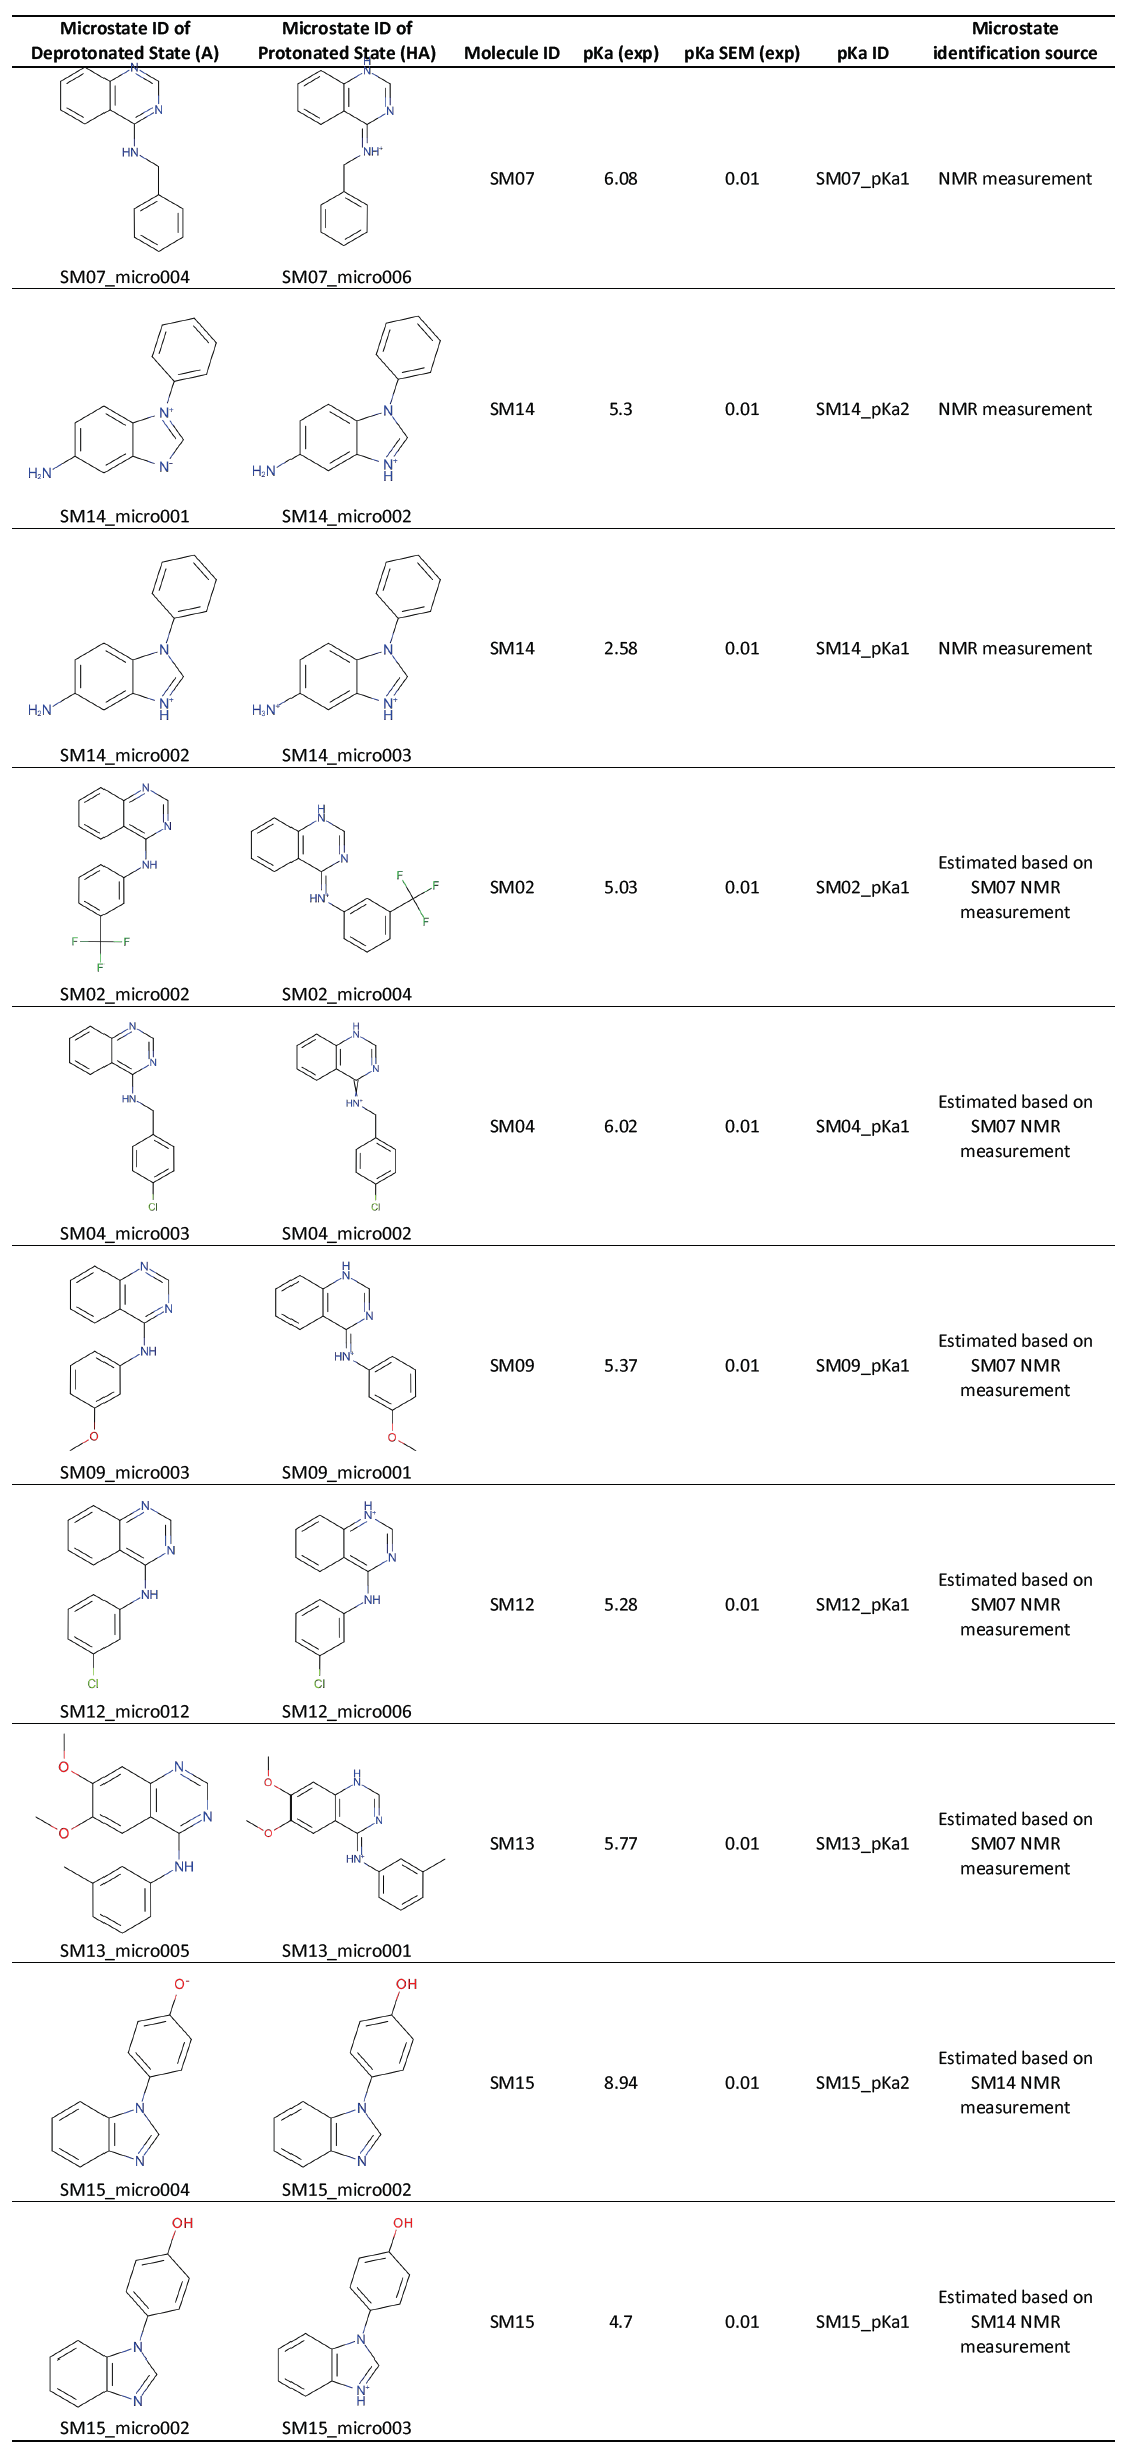
\includegraphics[width=0.5\linewidth]{figures/experimental-microstates-of-8mol-based-on-NMR.png}
\caption{ {\bf Dominant microstates of 8 molecules were determined based on NMR measurements.} Dominant microstate sequence of 6 derivatives were determined taking SM07 and SM14 as reference. Matched experimental \pKa{} values were determined by spectrophotometric \pKa{} measurements~\citep{Isik:2018:J.Comput.AidedMol.Des.}. A CSV version of this table can be found in \textit{SAMPL6-supplementary-documents.tar.gz}.
}
\label{fig:experimental-microstate-IDs-SI-table}
\end{figure}


\begin{figure}
\centering
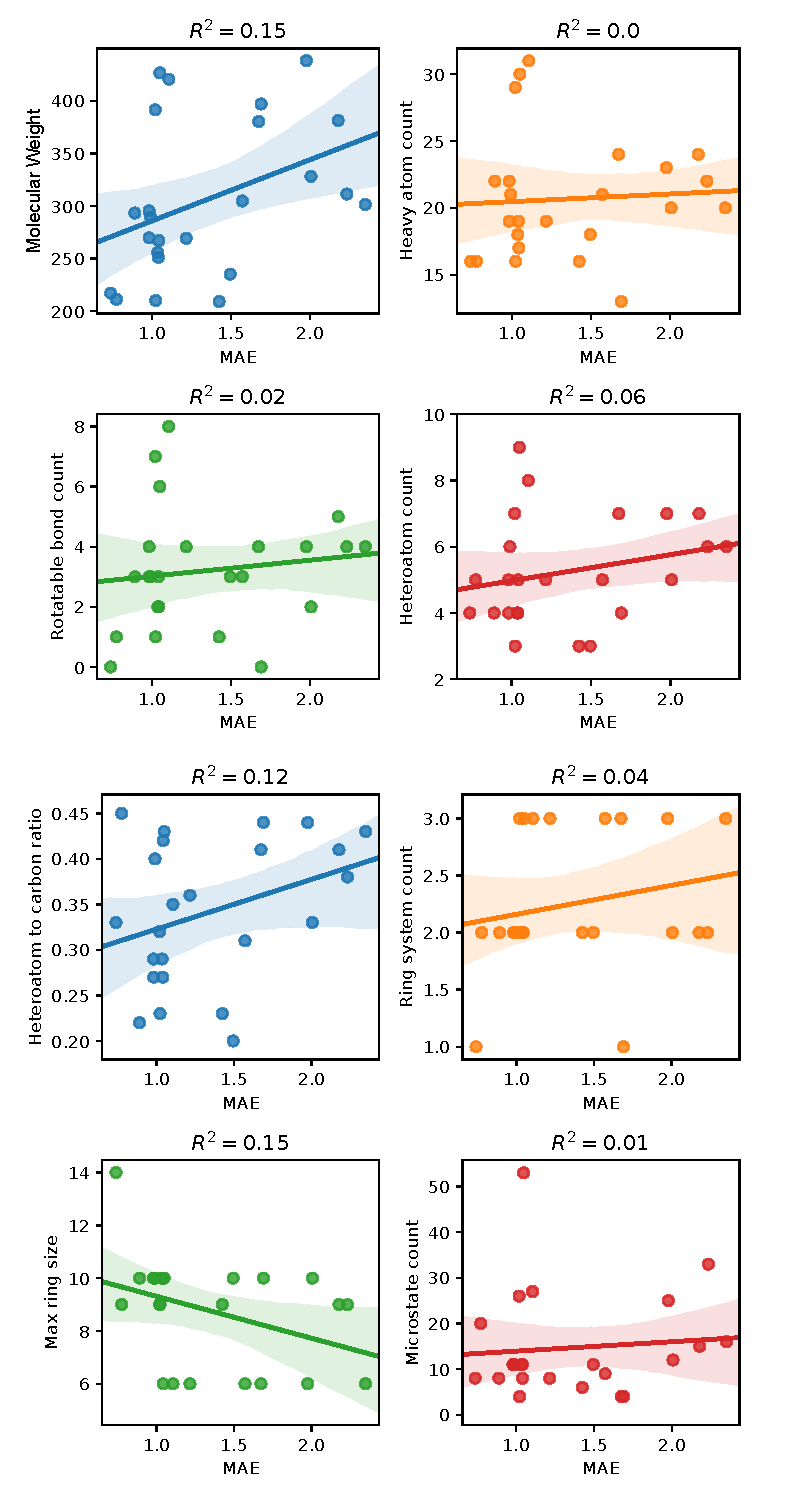
\includegraphics[width=0.5\linewidth]{figures/molecular_properties_vs_MAE_correlation_fig.pdf}
\caption{ {\bf MAE of macroscopic \pKa{} predictions of each molecule did not show any significant correlation with any molecular descriptor.} Plots show regression lines, 96\% confidence intervals of the regression lines, and R\textsubscript{2}. The following molecular descriptors were calculated using OpenEye OEMolProp Toolkit~\citep{oemolprop_openeye_2017}.
}
\label{fig:molecular_properties_vs_MAE_correlation}
\end{figure}


\begin{figure}
\centering
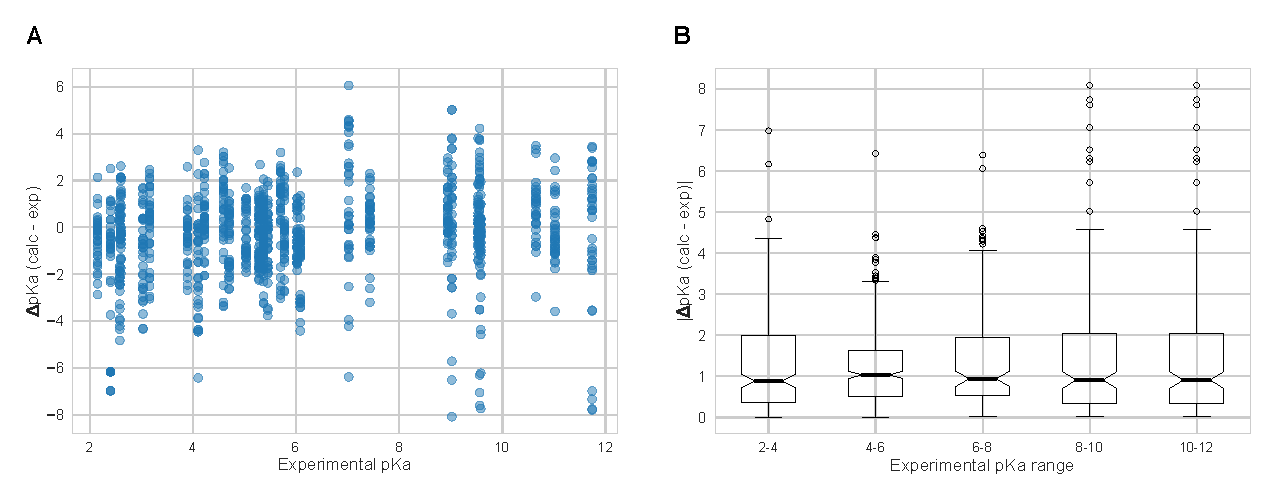
\includegraphics[width=1.0\linewidth]{figures/typeIII_error_vs_exp_pKa.pdf}
\caption{ {\bf The value of macroscopic \pKa{}s was not a factor affecting prediction error seen in SAMPL6 Challenge according to the analysis with Hungarian matching.} There was not clear trend between \pKa{} prediction error and the true \pKa{} error. Very high and very low \pKa{} values have similar inaccuracy compared to \pKa{} values close to 7. {\bf A} Scatter plot of macroscopic \pKa{} prediction error calculated with Hungarian matching vs. experimental \pKa{} value {\bf B} Box plot of absolute error of macroscopic \pKa{} predictions binned into 2 \pKa{} unit intervals of experimental \pKa{}.
}
\label{fig:macroscopic-pKa-error-vs-pKa-value}
\end{figure}


\begin{figure}
\centering
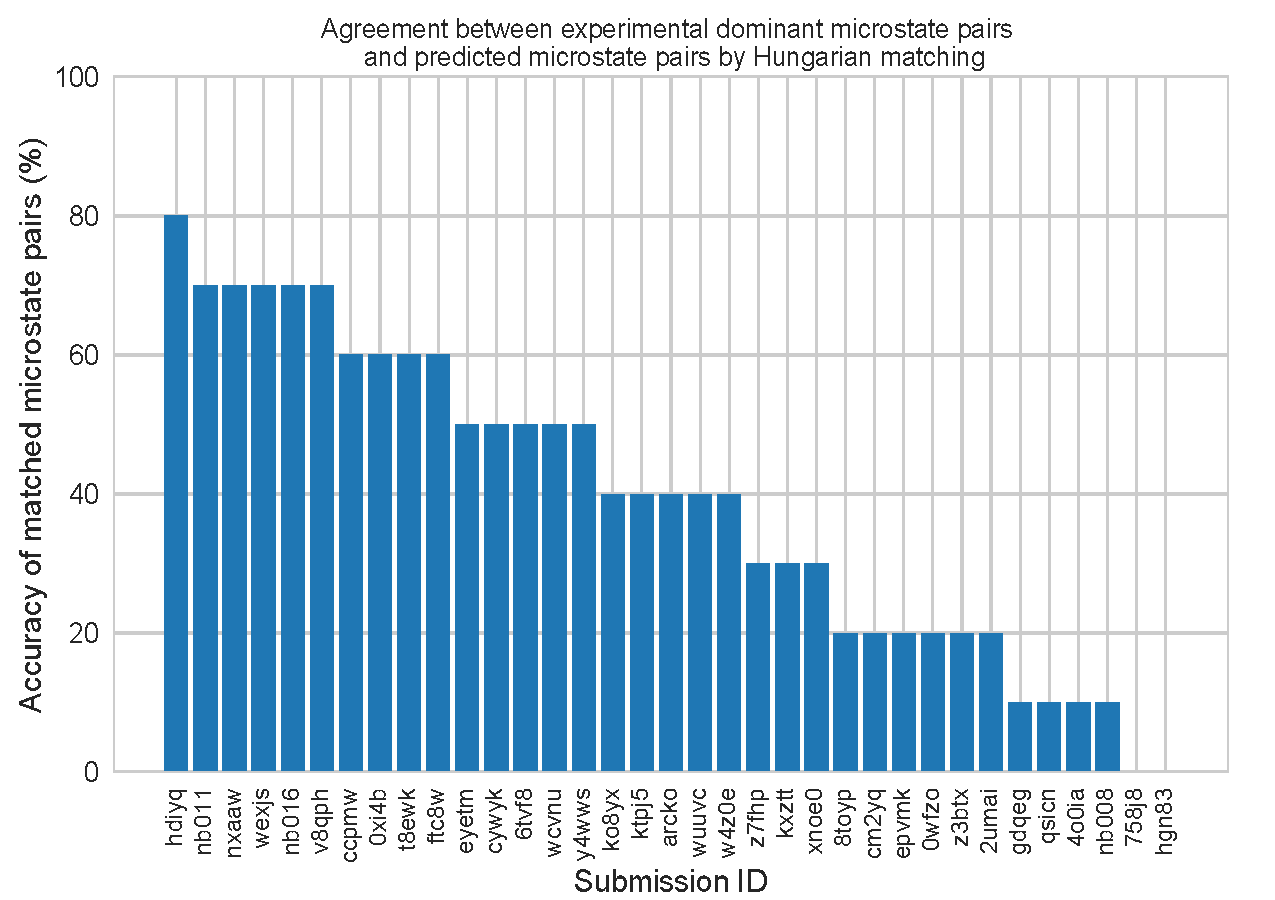
\includegraphics[width=0.75\linewidth]{figures/TypeI_Hungarian_match_microstate_pair_accuracy.pdf}
\caption{ {\bf There was low agreement between experimental dominant microstate pairs and the predicted microstate pairs selected by Hungarian algorithm for microscopic \pKa{} predictions.} This analysis could only be performed for 8 molecules with NMR data. Hungarian matching algorithm which matches predicted and experimental values considering only the closeness of the numerical value of \pKa{} and it often leds to predicted \pKa{} matches that described a different microstates pair than the experimentally observed dominant microstates..
}
\label{fig:microstate-pairs-with-Hungarian-match-vs-experiments}
\end{figure}



\end{document}
